\documentclass[twoside]{article}

% Packages required by doxygen
\usepackage{fixltx2e}
\usepackage{calc}
\usepackage{doxygen}
\usepackage[export]{adjustbox} % also loads graphicx
\usepackage{graphicx}
\usepackage[utf8]{inputenc}
\usepackage{makeidx}
\usepackage{multicol}
\usepackage{multirow}
\PassOptionsToPackage{warn}{textcomp}
\usepackage{textcomp}
\usepackage[nointegrals]{wasysym}
\usepackage[table]{xcolor}

% Font selection
\usepackage[T1]{fontenc}
\usepackage[scaled=.90]{helvet}
\usepackage{courier}
\usepackage{amssymb}
\usepackage{sectsty}
\renewcommand{\familydefault}{\sfdefault}
\allsectionsfont{%
  \fontseries{bc}\selectfont%
  \color{darkgray}%
}
\renewcommand{\DoxyLabelFont}{%
  \fontseries{bc}\selectfont%
  \color{darkgray}%
}
\newcommand{\+}{\discretionary{\mbox{\scriptsize$\hookleftarrow$}}{}{}}

% Page & text layout
\usepackage{geometry}
\geometry{%
  a4paper,%
  top=2.5cm,%
  bottom=2.5cm,%
  left=2.5cm,%
  right=2.5cm%
}
\tolerance=750
\hfuzz=15pt
\hbadness=750
\setlength{\emergencystretch}{15pt}
\setlength{\parindent}{0cm}
\setlength{\parskip}{3ex plus 2ex minus 2ex}
\makeatletter
\renewcommand{\paragraph}{%
  \@startsection{paragraph}{4}{0ex}{-1.0ex}{1.0ex}{%
    \normalfont\normalsize\bfseries\SS@parafont%
  }%
}
\renewcommand{\subparagraph}{%
  \@startsection{subparagraph}{5}{0ex}{-1.0ex}{1.0ex}{%
    \normalfont\normalsize\bfseries\SS@subparafont%
  }%
}
\makeatother

% Headers & footers
\usepackage{fancyhdr}
\pagestyle{fancyplain}
\fancyhead[LE]{\fancyplain{}{\bfseries\thepage}}
\fancyhead[CE]{\fancyplain{}{}}
\fancyhead[RE]{\fancyplain{}{\bfseries\leftmark}}
\fancyhead[LO]{\fancyplain{}{\bfseries\rightmark}}
\fancyhead[CO]{\fancyplain{}{}}
\fancyhead[RO]{\fancyplain{}{\bfseries\thepage}}
\fancyfoot[LE]{\fancyplain{}{}}
\fancyfoot[CE]{\fancyplain{}{}}
\fancyfoot[RE]{\fancyplain{}{\bfseries\scriptsize Generated by Doxygen }}
\fancyfoot[LO]{\fancyplain{}{\bfseries\scriptsize Generated by Doxygen }}
\fancyfoot[CO]{\fancyplain{}{}}
\fancyfoot[RO]{\fancyplain{}{}}
\renewcommand{\footrulewidth}{0.4pt}
\renewcommand{\sectionmark}[1]{%
  \markright{\thesection\ #1}%
}

% Indices & bibliography
\usepackage{natbib}
\usepackage[titles]{tocloft}
\setcounter{tocdepth}{3}
\setcounter{secnumdepth}{5}
\makeindex

% Packages requested by user
\usepackage{times,}
\usepackage{amsmath,}
\usepackage{tikz}

% Hyperlinks (required, but should be loaded last)
\usepackage{ifpdf}
\ifpdf
  \usepackage[pdftex,pagebackref=true]{hyperref}
\else
  \usepackage[ps2pdf,pagebackref=true]{hyperref}
\fi
\hypersetup{%
  colorlinks=true,%
  linkcolor=blue,%
  citecolor=blue,%
  unicode%
}

% Custom commands
\newcommand{\clearemptydoublepage}{%
  \newpage{\pagestyle{empty}\cleardoublepage}%
}

\usepackage{caption}
\captionsetup{labelsep=space,justification=centering,font={bf},singlelinecheck=off,skip=4pt,position=top}

%===== C O N T E N T S =====

\begin{document}

% Titlepage & ToC
\hypersetup{pageanchor=false,
             bookmarksnumbered=true,
             pdfencoding=unicode
            }
\pagenumbering{alph}
\begin{titlepage}
\vspace*{7cm}
\begin{center}%
{\Large Distributed Q\+U\+E\+ST for G\+PU }\\
\vspace*{1cm}
{\large Generated by Doxygen 1.8.14}\\
\end{center}
\end{titlepage}
\pagenumbering{roman}
\tableofcontents
\pagenumbering{arabic}
\hypersetup{pageanchor=true}

%--- Begin generated contents ---
\section{Qu\+E\+ST for G\+PU}
\label{index}\hypertarget{index}{}\subsubsection*{Versions}

Qu\+E\+ST is currently in prerelease and may be unstable. ~\newline
 Latest version\+: \href{https://github.com/aniabrown/QuEST_GPU/releases/tag/v0.7.0}{\tt 0.\+7.\+0}

This is the repository for the G\+PU version of the code. The C\+PU version is available \href{https://github.com/aniabrown/QuEST}{\tt here}. The G\+PU version is behind the C\+PU version -- the full A\+PI is listed \href{https://aniabrown.github.io/QuEST/qubits_8h.html}{\tt here} and the subset of this implemented for the G\+PU is listed \href{https://aniabrown.github.io/QuEST_GPU/qubits_8h.html}{\tt here}.

Please report errors or feedback to \href{mailto:anna.brown@oerc.ox.ac.uk}{\tt anna.\+brown@oerc.\+ox.\+ac.\+uk}

\subsubsection*{Introduction}

The {\bfseries Quantum Exact Simulation Toolkit} is a high performance simulator of universal quantum circuits. Qu\+E\+ST is written in C, hybridises Open\+MP and M\+PI, and can run on a G\+PU. Needing only compilation, Qu\+E\+ST is easy to run both on laptops and supercomputers, where it can take advantage of multicore and networked machines to quickly simulate circuits on many qubits.

Qu\+E\+ST has a simple interface, independent of its run environment (on C\+P\+Us, G\+P\+Us or over networks), 
\begin{DoxyCode}
\mbox{\hyperlink{QuEST_8h_aa09b5dd93de6df1384b8f2c0041749ab}{hadamard}}(qubits, 0);

\mbox{\hyperlink{QuEST_8h_a67576895bbc65463481a8ea24d9b1e22}{controlledNot}}(qubits, 0, 1);

\mbox{\hyperlink{QuEST_8cpp_ace0d3592d38a990e81a434c4e9681500}{rotateY}}(qubits, 0, .1);
\end{DoxyCode}
 though is flexible 
\begin{DoxyCode}
\mbox{\hyperlink{structVector}{Vector}} v;
v.\mbox{\hyperlink{structVector_aac7abe171ba4bada50ed72acba6259fc}{x}} = 1; v.\mbox{\hyperlink{structVector_a375ca805d4c808a53d7c4e0c737ae3de}{y}} = 0; v.\mbox{\hyperlink{structVector_ad4e863651be7d6b7e2b28cd7445a0ccf}{z}} = 0;
\mbox{\hyperlink{QuEST_8cpp_a8810423457803005fecd415f4299f40d}{rotateAroundAxis}}(qubits, 0, 3.14/2, v);
\end{DoxyCode}
 and powerful 
\begin{DoxyCode}
\mbox{\hyperlink{structComplexMatrix2}{ComplexMatrix2}} u;
u.\mbox{\hyperlink{structComplexMatrix2_ae72b4458233b077a636beee1892e81ff}{r0c0}} = (\mbox{\hyperlink{QuEST_8h_ad59c9e471673c07782e6c403277ffd8d}{Complex}}) \{.\mbox{\hyperlink{structComplex_a479ad939835457595fcca3ca55c06283}{real}}=.5, .imag= .5\};
u.\mbox{\hyperlink{structComplexMatrix2_a0f3932f055a8b05cef361bce25d51172}{r0c1}} = (\mbox{\hyperlink{QuEST_8h_ad59c9e471673c07782e6c403277ffd8d}{Complex}}) \{.\mbox{\hyperlink{structComplex_a479ad939835457595fcca3ca55c06283}{real}}=.5, .imag=-.5\}; 
u.\mbox{\hyperlink{structComplexMatrix2_ab98282015ed2065e53fbc9638e2583ab}{r1c0}} = (\mbox{\hyperlink{QuEST_8h_ad59c9e471673c07782e6c403277ffd8d}{Complex}}) \{.\mbox{\hyperlink{structComplex_a479ad939835457595fcca3ca55c06283}{real}}=.5, .imag=-.5\};
u.\mbox{\hyperlink{structComplexMatrix2_a763007c3070802373549ba0350f83c8a}{r1c1}} = (\mbox{\hyperlink{QuEST_8h_ad59c9e471673c07782e6c403277ffd8d}{Complex}}) \{.\mbox{\hyperlink{structComplex_a479ad939835457595fcca3ca55c06283}{real}}=.5, .imag= .5\};
\mbox{\hyperlink{QuEST_8h_a7a0877e33700f6bad48adb51b7b3fb67}{unitary}}(qubits, 0, u);

\textcolor{keywordtype}{int}[] controls = \{1, 2, 3, 4, 5\};
\mbox{\hyperlink{QuEST_8h_ae395a79690283ed81106afadd7a8cd8a}{multiControlledUnitary}}(qureg, controls, 5, 0, u);
\end{DoxyCode}


\subsubsection*{Getting started}

Qu\+E\+ST is contained entirely in the {\ttfamily .c} and {\ttfamily .h} files in the {\ttfamily Qu\+E\+S\+T/} folder. To use Qu\+E\+ST, copy these files to your computer and include {\ttfamily qubits.\+h} in your C code. We include make files for compiling Qu\+E\+ST, and submission scripts for using Qu\+E\+ST with S\+L\+U\+RM and P\+BS. See /examples/tutorial.md \char`\"{}examples/tutorial.\+md\char`\"{} for an introduction. Clone or download this entire repository to include all examples as well as tests and documentation.

\subsubsection*{A\+PI Documentation}

View the A\+PI for the G\+PU version \href{https://aniabrown.github.io/QuEST_GPU/qubits_8h.html}{\tt here}, and the full documentation at \href{https://aniabrown.github.io/QuEST_GPU/}{\tt https\+://aniabrown.\+github.\+io/\+Qu\+E\+S\+T\+\_\+\+G\+P\+U/}

\subsubsection*{Licence}

Qu\+E\+ST is released under a \href{LICENCE.txt}{\tt M\+IT Licence} 
\section{Data Structure Index}
\subsection{Data Structures}
Here are the data structures with brief descriptions\+:\begin{DoxyCompactList}
\item\contentsline{section}{\mbox{\hyperlink{structComplex}{Complex}} \\*Represents one complex number }{\pageref{structComplex}}{}
\item\contentsline{section}{\mbox{\hyperlink{structComplexArray}{Complex\+Array}} \\*Represents an array of complex numbers grouped into an array of real components and an array of coressponding complex components }{\pageref{structComplexArray}}{}
\item\contentsline{section}{\mbox{\hyperlink{structComplexMatrix2}{Complex\+Matrix2}} \\*Represents a 2x2 matrix of complex numbers }{\pageref{structComplexMatrix2}}{}
\item\contentsline{section}{\mbox{\hyperlink{structMultiQubit}{Multi\+Qubit}} \\*Represents a system of qubits }{\pageref{structMultiQubit}}{}
\item\contentsline{section}{\mbox{\hyperlink{structQuESTEnv}{Qu\+E\+S\+T\+Env}} \\*Information about the environment the program is running in }{\pageref{structQuESTEnv}}{}
\item\contentsline{section}{\mbox{\hyperlink{structVector}{Vector}} }{\pageref{structVector}}{}
\end{DoxyCompactList}

\section{File Index}
\subsection{File List}
Here is a list of all files with brief descriptions:\begin{DoxyCompactList}
\item\contentsline{section}{\hyperlink{README_8md}{README.md} }{\pageref{README_8md}}{}
\item\contentsline{section}{\hyperlink{runTests_8cpp}{runTests.cpp} }{\pageref{runTests_8cpp}}{}
\end{DoxyCompactList}

\section{Data Structure Documentation}
\hypertarget{structComplex}{}\subsection{Complex Struct Reference}
\label{structComplex}\index{Complex@{Complex}}


Represents one complex number.  




{\ttfamily \#include $<$qubits.\+h$>$}

\subsubsection*{Data Fields}
\begin{DoxyCompactItemize}
\item 
\mbox{\hyperlink{precision_8h_a4b654506f18b8bfd61ad2a29a7e38c25}{R\+E\+AL}} \mbox{\hyperlink{structComplex_a479ad939835457595fcca3ca55c06283}{real}}
\item 
\mbox{\hyperlink{precision_8h_a4b654506f18b8bfd61ad2a29a7e38c25}{R\+E\+AL}} \mbox{\hyperlink{structComplex_a1151948284b21c0052f203f23ab931d9}{imag}}
\end{DoxyCompactItemize}


\subsubsection{Detailed Description}
Represents one complex number. 

Definition at line 22 of file qubits.\+h.



\subsubsection{Field Documentation}
\mbox{\Hypertarget{structComplex_a1151948284b21c0052f203f23ab931d9}\label{structComplex_a1151948284b21c0052f203f23ab931d9}} 
\index{Complex@{Complex}!imag@{imag}}
\index{imag@{imag}!Complex@{Complex}}
\paragraph{\texorpdfstring{imag}{imag}}
{\footnotesize\ttfamily \mbox{\hyperlink{precision_8h_a4b654506f18b8bfd61ad2a29a7e38c25}{R\+E\+AL}} Complex\+::imag}



Definition at line 25 of file qubits.\+h.



Referenced by controlled\+Rotate\+Around\+Axis(), main(), rotate\+Around\+Axis(), validate\+Alpha\+Beta(), and validate\+Matrix\+Is\+Unitary().

\mbox{\Hypertarget{structComplex_a479ad939835457595fcca3ca55c06283}\label{structComplex_a479ad939835457595fcca3ca55c06283}} 
\index{Complex@{Complex}!real@{real}}
\index{real@{real}!Complex@{Complex}}
\paragraph{\texorpdfstring{real}{real}}
{\footnotesize\ttfamily \mbox{\hyperlink{precision_8h_a4b654506f18b8bfd61ad2a29a7e38c25}{R\+E\+AL}} Complex\+::real}



Definition at line 24 of file qubits.\+h.



Referenced by controlled\+Rotate\+Around\+Axis(), main(), rotate\+Around\+Axis(), validate\+Alpha\+Beta(), and validate\+Matrix\+Is\+Unitary().



The documentation for this struct was generated from the following file\+:\begin{DoxyCompactItemize}
\item 
\mbox{\hyperlink{qubits_8h}{qubits.\+h}}\end{DoxyCompactItemize}

\hypertarget{structComplexArray}{}\subsection{Complex\+Array Struct Reference}
\label{structComplexArray}\index{Complex\+Array@{Complex\+Array}}


Represents an array of complex numbers grouped into an array of real components and an array of coressponding complex components.  




{\ttfamily \#include $<$Qu\+E\+S\+T.\+h$>$}

\subsubsection*{Data Fields}
\begin{DoxyCompactItemize}
\item 
\mbox{\hyperlink{QuEST__precision_8h_a4b654506f18b8bfd61ad2a29a7e38c25}{R\+E\+AL}} $\ast$ \mbox{\hyperlink{structComplexArray_a4195cac6c784ea1b6271f1c7dba1548a}{real}}
\item 
\mbox{\hyperlink{QuEST__precision_8h_a4b654506f18b8bfd61ad2a29a7e38c25}{R\+E\+AL}} $\ast$ \mbox{\hyperlink{structComplexArray_a79dde47c7ae530c79cebfdf57b225968}{imag}}
\end{DoxyCompactItemize}


\subsubsection{Detailed Description}
Represents an array of complex numbers grouped into an array of real components and an array of coressponding complex components. 

Definition at line 18 of file Qu\+E\+S\+T.\+h.



\subsubsection{Field Documentation}
\mbox{\Hypertarget{structComplexArray_a79dde47c7ae530c79cebfdf57b225968}\label{structComplexArray_a79dde47c7ae530c79cebfdf57b225968}} 
\index{Complex\+Array@{Complex\+Array}!imag@{imag}}
\index{imag@{imag}!Complex\+Array@{Complex\+Array}}
\paragraph{\texorpdfstring{imag}{imag}}
{\footnotesize\ttfamily \mbox{\hyperlink{QuEST__precision_8h_a4b654506f18b8bfd61ad2a29a7e38c25}{R\+E\+AL}}$\ast$ Complex\+Array\+::imag}



Definition at line 21 of file Qu\+E\+S\+T.\+h.



Referenced by report\+State().

\mbox{\Hypertarget{structComplexArray_a4195cac6c784ea1b6271f1c7dba1548a}\label{structComplexArray_a4195cac6c784ea1b6271f1c7dba1548a}} 
\index{Complex\+Array@{Complex\+Array}!real@{real}}
\index{real@{real}!Complex\+Array@{Complex\+Array}}
\paragraph{\texorpdfstring{real}{real}}
{\footnotesize\ttfamily \mbox{\hyperlink{QuEST__precision_8h_a4b654506f18b8bfd61ad2a29a7e38c25}{R\+E\+AL}}$\ast$ Complex\+Array\+::real}



Definition at line 20 of file Qu\+E\+S\+T.\+h.



Referenced by report\+State().



The documentation for this struct was generated from the following file\+:\begin{DoxyCompactItemize}
\item 
\mbox{\hyperlink{QuEST_8h}{Qu\+E\+S\+T.\+h}}\end{DoxyCompactItemize}

\hypertarget{structComplexMatrix2}{}\subsection{Complex\+Matrix2 Struct Reference}
\label{structComplexMatrix2}\index{Complex\+Matrix2@{Complex\+Matrix2}}


Represents a 2x2 matrix of complex numbers.  




{\ttfamily \#include $<$qubits.\+h$>$}

\subsubsection*{Data Fields}
\begin{DoxyCompactItemize}
\item 
\mbox{\hyperlink{structComplex}{Complex}} \mbox{\hyperlink{structComplexMatrix2_ae72b4458233b077a636beee1892e81ff}{r0c0}}
\item 
\mbox{\hyperlink{structComplex}{Complex}} \mbox{\hyperlink{structComplexMatrix2_a0f3932f055a8b05cef361bce25d51172}{r0c1}}
\item 
\mbox{\hyperlink{structComplex}{Complex}} \mbox{\hyperlink{structComplexMatrix2_ab98282015ed2065e53fbc9638e2583ab}{r1c0}}
\item 
\mbox{\hyperlink{structComplex}{Complex}} \mbox{\hyperlink{structComplexMatrix2_a763007c3070802373549ba0350f83c8a}{r1c1}}
\end{DoxyCompactItemize}


\subsubsection{Detailed Description}
Represents a 2x2 matrix of complex numbers. 

Definition at line 30 of file qubits.\+h.



\subsubsection{Field Documentation}
\mbox{\Hypertarget{structComplexMatrix2_ae72b4458233b077a636beee1892e81ff}\label{structComplexMatrix2_ae72b4458233b077a636beee1892e81ff}} 
\index{Complex\+Matrix2@{Complex\+Matrix2}!r0c0@{r0c0}}
\index{r0c0@{r0c0}!Complex\+Matrix2@{Complex\+Matrix2}}
\paragraph{\texorpdfstring{r0c0}{r0c0}}
{\footnotesize\ttfamily \mbox{\hyperlink{structComplex}{Complex}} Complex\+Matrix2\+::r0c0}



Definition at line 32 of file qubits.\+h.



Referenced by validate\+Matrix\+Is\+Unitary().

\mbox{\Hypertarget{structComplexMatrix2_a0f3932f055a8b05cef361bce25d51172}\label{structComplexMatrix2_a0f3932f055a8b05cef361bce25d51172}} 
\index{Complex\+Matrix2@{Complex\+Matrix2}!r0c1@{r0c1}}
\index{r0c1@{r0c1}!Complex\+Matrix2@{Complex\+Matrix2}}
\paragraph{\texorpdfstring{r0c1}{r0c1}}
{\footnotesize\ttfamily \mbox{\hyperlink{structComplex}{Complex}} Complex\+Matrix2\+::r0c1}



Definition at line 32 of file qubits.\+h.



Referenced by validate\+Matrix\+Is\+Unitary().

\mbox{\Hypertarget{structComplexMatrix2_ab98282015ed2065e53fbc9638e2583ab}\label{structComplexMatrix2_ab98282015ed2065e53fbc9638e2583ab}} 
\index{Complex\+Matrix2@{Complex\+Matrix2}!r1c0@{r1c0}}
\index{r1c0@{r1c0}!Complex\+Matrix2@{Complex\+Matrix2}}
\paragraph{\texorpdfstring{r1c0}{r1c0}}
{\footnotesize\ttfamily \mbox{\hyperlink{structComplex}{Complex}} Complex\+Matrix2\+::r1c0}



Definition at line 33 of file qubits.\+h.



Referenced by validate\+Matrix\+Is\+Unitary().

\mbox{\Hypertarget{structComplexMatrix2_a763007c3070802373549ba0350f83c8a}\label{structComplexMatrix2_a763007c3070802373549ba0350f83c8a}} 
\index{Complex\+Matrix2@{Complex\+Matrix2}!r1c1@{r1c1}}
\index{r1c1@{r1c1}!Complex\+Matrix2@{Complex\+Matrix2}}
\paragraph{\texorpdfstring{r1c1}{r1c1}}
{\footnotesize\ttfamily \mbox{\hyperlink{structComplex}{Complex}} Complex\+Matrix2\+::r1c1}



Definition at line 33 of file qubits.\+h.



Referenced by validate\+Matrix\+Is\+Unitary().



The documentation for this struct was generated from the following file\+:\begin{DoxyCompactItemize}
\item 
\mbox{\hyperlink{qubits_8h}{qubits.\+h}}\end{DoxyCompactItemize}

\hypertarget{structMultiQubit}{}\subsection{Multi\+Qubit Struct Reference}
\label{structMultiQubit}\index{Multi\+Qubit@{Multi\+Qubit}}


Represents a system of qubits.  




{\ttfamily \#include $<$Qu\+E\+S\+T.\+h$>$}

\subsubsection*{Data Fields}
\begin{DoxyCompactItemize}
\item 
\mbox{\hyperlink{structComplexArray}{Complex\+Array}} \mbox{\hyperlink{structMultiQubit_a45483190d6b01ef6b2f98f2bec9ab94f}{state\+Vec}}
\begin{DoxyCompactList}\small\item\em Probablilty amplitudes for the multi qubit state. \end{DoxyCompactList}\item 
\mbox{\hyperlink{structComplexArray}{Complex\+Array}} \mbox{\hyperlink{structMultiQubit_a76f7db4eab52d2b30f58f973ada809c5}{pair\+State\+Vec}}
\begin{DoxyCompactList}\small\item\em Temporary storage for a chunk of the state vector received from another process in the M\+PI version. \end{DoxyCompactList}\item 
\mbox{\hyperlink{structComplexArray}{Complex\+Array}} \mbox{\hyperlink{structMultiQubit_a59ac613486a41b8c9a4b6e79cc8d2cc3}{device\+State\+Vec}}
\begin{DoxyCompactList}\small\item\em Storage for probability amplitudes for the multi qubit state on G\+PU. \end{DoxyCompactList}\item 
\mbox{\hyperlink{QuEST__precision_8h_a4b654506f18b8bfd61ad2a29a7e38c25}{R\+E\+AL}} $\ast$ \mbox{\hyperlink{structMultiQubit_a4e0088b41adab0a40b7a31e528ed42b5}{first\+Level\+Reduction}}
\begin{DoxyCompactList}\small\item\em Storage for reduction of probabilities on G\+PU. \end{DoxyCompactList}\item 
\mbox{\hyperlink{QuEST__precision_8h_a4b654506f18b8bfd61ad2a29a7e38c25}{R\+E\+AL}} $\ast$ \mbox{\hyperlink{structMultiQubit_a3e859cefa146ec7b30464ab3d897930b}{second\+Level\+Reduction}}
\item 
int \mbox{\hyperlink{structMultiQubit_ab5b9795bdc6fb5855e1974dcbbaeb36f}{num\+Qubits}}
\begin{DoxyCompactList}\small\item\em Number of qubits in the state. \end{DoxyCompactList}\item 
long long int \mbox{\hyperlink{structMultiQubit_ae16f47d8b725c914fb7f66b6498d79db}{num\+Amps}}
\begin{DoxyCompactList}\small\item\em Number of probability amplitudes held in state\+Vec by this process In the non-\/\+M\+PI version, this is the total number of amplitudes. \end{DoxyCompactList}\item 
int \mbox{\hyperlink{structMultiQubit_ab10c88249fa3825d6227ceec01d37e37}{chunk\+Id}}
\begin{DoxyCompactList}\small\item\em The position of the chunk of the state vector held by this process in the full state vector. \end{DoxyCompactList}\item 
int \mbox{\hyperlink{structMultiQubit_acd43f2f57991709c9e94f73662c972b2}{num\+Chunks}}
\begin{DoxyCompactList}\small\item\em Number of chunks the state vector is broken up into -- the number of M\+PI processes used. \end{DoxyCompactList}\end{DoxyCompactItemize}


\subsubsection{Detailed Description}
Represents a system of qubits. 

Qubits are zero-\/based and the the first qubit is the rightmost 

Definition at line 48 of file Qu\+E\+S\+T.\+h.



\subsubsection{Field Documentation}
\mbox{\Hypertarget{structMultiQubit_ab10c88249fa3825d6227ceec01d37e37}\label{structMultiQubit_ab10c88249fa3825d6227ceec01d37e37}} 
\index{Multi\+Qubit@{Multi\+Qubit}!chunk\+Id@{chunk\+Id}}
\index{chunk\+Id@{chunk\+Id}!Multi\+Qubit@{Multi\+Qubit}}
\paragraph{\texorpdfstring{chunk\+Id}{chunkId}}
{\footnotesize\ttfamily int Multi\+Qubit\+::chunk\+Id}



The position of the chunk of the state vector held by this process in the full state vector. 



Definition at line 64 of file Qu\+E\+S\+T.\+h.



Referenced by report\+Multi\+Qubit\+Params(), and report\+State().

\mbox{\Hypertarget{structMultiQubit_a59ac613486a41b8c9a4b6e79cc8d2cc3}\label{structMultiQubit_a59ac613486a41b8c9a4b6e79cc8d2cc3}} 
\index{Multi\+Qubit@{Multi\+Qubit}!device\+State\+Vec@{device\+State\+Vec}}
\index{device\+State\+Vec@{device\+State\+Vec}!Multi\+Qubit@{Multi\+Qubit}}
\paragraph{\texorpdfstring{device\+State\+Vec}{deviceStateVec}}
{\footnotesize\ttfamily \mbox{\hyperlink{structComplexArray}{Complex\+Array}} Multi\+Qubit\+::device\+State\+Vec}



Storage for probability amplitudes for the multi qubit state on G\+PU. 



Definition at line 55 of file Qu\+E\+S\+T.\+h.

\mbox{\Hypertarget{structMultiQubit_a4e0088b41adab0a40b7a31e528ed42b5}\label{structMultiQubit_a4e0088b41adab0a40b7a31e528ed42b5}} 
\index{Multi\+Qubit@{Multi\+Qubit}!first\+Level\+Reduction@{first\+Level\+Reduction}}
\index{first\+Level\+Reduction@{first\+Level\+Reduction}!Multi\+Qubit@{Multi\+Qubit}}
\paragraph{\texorpdfstring{first\+Level\+Reduction}{firstLevelReduction}}
{\footnotesize\ttfamily \mbox{\hyperlink{QuEST__precision_8h_a4b654506f18b8bfd61ad2a29a7e38c25}{R\+E\+AL}}$\ast$ Multi\+Qubit\+::first\+Level\+Reduction}



Storage for reduction of probabilities on G\+PU. 



Definition at line 57 of file Qu\+E\+S\+T.\+h.

\mbox{\Hypertarget{structMultiQubit_ae16f47d8b725c914fb7f66b6498d79db}\label{structMultiQubit_ae16f47d8b725c914fb7f66b6498d79db}} 
\index{Multi\+Qubit@{Multi\+Qubit}!num\+Amps@{num\+Amps}}
\index{num\+Amps@{num\+Amps}!Multi\+Qubit@{Multi\+Qubit}}
\paragraph{\texorpdfstring{num\+Amps}{numAmps}}
{\footnotesize\ttfamily long long int Multi\+Qubit\+::num\+Amps}



Number of probability amplitudes held in state\+Vec by this process In the non-\/\+M\+PI version, this is the total number of amplitudes. 



Definition at line 62 of file Qu\+E\+S\+T.\+h.



Referenced by report\+State().

\mbox{\Hypertarget{structMultiQubit_acd43f2f57991709c9e94f73662c972b2}\label{structMultiQubit_acd43f2f57991709c9e94f73662c972b2}} 
\index{Multi\+Qubit@{Multi\+Qubit}!num\+Chunks@{num\+Chunks}}
\index{num\+Chunks@{num\+Chunks}!Multi\+Qubit@{Multi\+Qubit}}
\paragraph{\texorpdfstring{num\+Chunks}{numChunks}}
{\footnotesize\ttfamily int Multi\+Qubit\+::num\+Chunks}



Number of chunks the state vector is broken up into -- the number of M\+PI processes used. 



Definition at line 66 of file Qu\+E\+S\+T.\+h.



Referenced by report\+Multi\+Qubit\+Params().

\mbox{\Hypertarget{structMultiQubit_ab5b9795bdc6fb5855e1974dcbbaeb36f}\label{structMultiQubit_ab5b9795bdc6fb5855e1974dcbbaeb36f}} 
\index{Multi\+Qubit@{Multi\+Qubit}!num\+Qubits@{num\+Qubits}}
\index{num\+Qubits@{num\+Qubits}!Multi\+Qubit@{Multi\+Qubit}}
\paragraph{\texorpdfstring{num\+Qubits}{numQubits}}
{\footnotesize\ttfamily int Multi\+Qubit\+::num\+Qubits}



Number of qubits in the state. 



Definition at line 59 of file Qu\+E\+S\+T.\+h.



Referenced by report\+Multi\+Qubit\+Params().

\mbox{\Hypertarget{structMultiQubit_a76f7db4eab52d2b30f58f973ada809c5}\label{structMultiQubit_a76f7db4eab52d2b30f58f973ada809c5}} 
\index{Multi\+Qubit@{Multi\+Qubit}!pair\+State\+Vec@{pair\+State\+Vec}}
\index{pair\+State\+Vec@{pair\+State\+Vec}!Multi\+Qubit@{Multi\+Qubit}}
\paragraph{\texorpdfstring{pair\+State\+Vec}{pairStateVec}}
{\footnotesize\ttfamily \mbox{\hyperlink{structComplexArray}{Complex\+Array}} Multi\+Qubit\+::pair\+State\+Vec}



Temporary storage for a chunk of the state vector received from another process in the M\+PI version. 



Definition at line 53 of file Qu\+E\+S\+T.\+h.

\mbox{\Hypertarget{structMultiQubit_a3e859cefa146ec7b30464ab3d897930b}\label{structMultiQubit_a3e859cefa146ec7b30464ab3d897930b}} 
\index{Multi\+Qubit@{Multi\+Qubit}!second\+Level\+Reduction@{second\+Level\+Reduction}}
\index{second\+Level\+Reduction@{second\+Level\+Reduction}!Multi\+Qubit@{Multi\+Qubit}}
\paragraph{\texorpdfstring{second\+Level\+Reduction}{secondLevelReduction}}
{\footnotesize\ttfamily \mbox{\hyperlink{QuEST__precision_8h_a4b654506f18b8bfd61ad2a29a7e38c25}{R\+E\+AL}} $\ast$ Multi\+Qubit\+::second\+Level\+Reduction}



Definition at line 57 of file Qu\+E\+S\+T.\+h.

\mbox{\Hypertarget{structMultiQubit_a45483190d6b01ef6b2f98f2bec9ab94f}\label{structMultiQubit_a45483190d6b01ef6b2f98f2bec9ab94f}} 
\index{Multi\+Qubit@{Multi\+Qubit}!state\+Vec@{state\+Vec}}
\index{state\+Vec@{state\+Vec}!Multi\+Qubit@{Multi\+Qubit}}
\paragraph{\texorpdfstring{state\+Vec}{stateVec}}
{\footnotesize\ttfamily \mbox{\hyperlink{structComplexArray}{Complex\+Array}} Multi\+Qubit\+::state\+Vec}



Probablilty amplitudes for the multi qubit state. 



Definition at line 51 of file Qu\+E\+S\+T.\+h.



Referenced by report\+State().



The documentation for this struct was generated from the following file\+:\begin{DoxyCompactItemize}
\item 
\mbox{\hyperlink{QuEST_8h}{Qu\+E\+S\+T.\+h}}\end{DoxyCompactItemize}

\hypertarget{structQuESTEnv}{}\subsection{Qu\+E\+S\+T\+Env Struct Reference}
\label{structQuESTEnv}\index{Qu\+E\+S\+T\+Env@{Qu\+E\+S\+T\+Env}}


Information about the environment the program is running in.  




{\ttfamily \#include $<$Qu\+E\+S\+T.\+h$>$}

\subsubsection*{Data Fields}
\begin{DoxyCompactItemize}
\item 
int \mbox{\hyperlink{structQuESTEnv_aa648bb336cf8598467cb62db00b9cee8}{rank}}
\item 
int \mbox{\hyperlink{structQuESTEnv_af22aacd7c9905accae28484785c193b4}{num\+Ranks}}
\end{DoxyCompactItemize}


\subsubsection{Detailed Description}
Information about the environment the program is running in. 

In practice, this holds info about M\+PI ranks and helps to hide M\+PI initialization code 

Definition at line 72 of file Qu\+E\+S\+T.\+h.



\subsubsection{Field Documentation}
\mbox{\Hypertarget{structQuESTEnv_af22aacd7c9905accae28484785c193b4}\label{structQuESTEnv_af22aacd7c9905accae28484785c193b4}} 
\index{Qu\+E\+S\+T\+Env@{Qu\+E\+S\+T\+Env}!num\+Ranks@{num\+Ranks}}
\index{num\+Ranks@{num\+Ranks}!Qu\+E\+S\+T\+Env@{Qu\+E\+S\+T\+Env}}
\paragraph{\texorpdfstring{num\+Ranks}{numRanks}}
{\footnotesize\ttfamily int Qu\+E\+S\+T\+Env\+::num\+Ranks}



Definition at line 75 of file Qu\+E\+S\+T.\+h.

\mbox{\Hypertarget{structQuESTEnv_aa648bb336cf8598467cb62db00b9cee8}\label{structQuESTEnv_aa648bb336cf8598467cb62db00b9cee8}} 
\index{Qu\+E\+S\+T\+Env@{Qu\+E\+S\+T\+Env}!rank@{rank}}
\index{rank@{rank}!Qu\+E\+S\+T\+Env@{Qu\+E\+S\+T\+Env}}
\paragraph{\texorpdfstring{rank}{rank}}
{\footnotesize\ttfamily int Qu\+E\+S\+T\+Env\+::rank}



Definition at line 74 of file Qu\+E\+S\+T.\+h.



The documentation for this struct was generated from the following file\+:\begin{DoxyCompactItemize}
\item 
\mbox{\hyperlink{QuEST_8h}{Qu\+E\+S\+T.\+h}}\end{DoxyCompactItemize}

\hypertarget{structVector}{}\subsection{Vector Struct Reference}
\label{structVector}\index{Vector@{Vector}}


{\ttfamily \#include $<$Qu\+E\+S\+T.\+h$>$}

\subsubsection*{Data Fields}
\begin{DoxyCompactItemize}
\item 
\mbox{\hyperlink{QuEST__precision_8h_a4b654506f18b8bfd61ad2a29a7e38c25}{R\+E\+AL}} \mbox{\hyperlink{structVector_aac7abe171ba4bada50ed72acba6259fc}{x}}
\item 
\mbox{\hyperlink{QuEST__precision_8h_a4b654506f18b8bfd61ad2a29a7e38c25}{R\+E\+AL}} \mbox{\hyperlink{structVector_a375ca805d4c808a53d7c4e0c737ae3de}{y}}
\item 
\mbox{\hyperlink{QuEST__precision_8h_a4b654506f18b8bfd61ad2a29a7e38c25}{R\+E\+AL}} \mbox{\hyperlink{structVector_ad4e863651be7d6b7e2b28cd7445a0ccf}{z}}
\end{DoxyCompactItemize}


\subsubsection{Detailed Description}


Definition at line 40 of file Qu\+E\+S\+T.\+h.



\subsubsection{Field Documentation}
\mbox{\Hypertarget{structVector_aac7abe171ba4bada50ed72acba6259fc}\label{structVector_aac7abe171ba4bada50ed72acba6259fc}} 
\index{Vector@{Vector}!x@{x}}
\index{x@{x}!Vector@{Vector}}
\paragraph{\texorpdfstring{x}{x}}
{\footnotesize\ttfamily \mbox{\hyperlink{QuEST__precision_8h_a4b654506f18b8bfd61ad2a29a7e38c25}{R\+E\+AL}} Vector\+::x}



Definition at line 42 of file Qu\+E\+S\+T.\+h.



Referenced by controlled\+Rotate\+Around\+Axis(), and rotate\+Around\+Axis().

\mbox{\Hypertarget{structVector_a375ca805d4c808a53d7c4e0c737ae3de}\label{structVector_a375ca805d4c808a53d7c4e0c737ae3de}} 
\index{Vector@{Vector}!y@{y}}
\index{y@{y}!Vector@{Vector}}
\paragraph{\texorpdfstring{y}{y}}
{\footnotesize\ttfamily \mbox{\hyperlink{QuEST__precision_8h_a4b654506f18b8bfd61ad2a29a7e38c25}{R\+E\+AL}} Vector\+::y}



Definition at line 42 of file Qu\+E\+S\+T.\+h.



Referenced by controlled\+Rotate\+Around\+Axis(), and rotate\+Around\+Axis().

\mbox{\Hypertarget{structVector_ad4e863651be7d6b7e2b28cd7445a0ccf}\label{structVector_ad4e863651be7d6b7e2b28cd7445a0ccf}} 
\index{Vector@{Vector}!z@{z}}
\index{z@{z}!Vector@{Vector}}
\paragraph{\texorpdfstring{z}{z}}
{\footnotesize\ttfamily \mbox{\hyperlink{QuEST__precision_8h_a4b654506f18b8bfd61ad2a29a7e38c25}{R\+E\+AL}} Vector\+::z}



Definition at line 42 of file Qu\+E\+S\+T.\+h.



Referenced by controlled\+Rotate\+Around\+Axis(), and rotate\+Around\+Axis().



The documentation for this struct was generated from the following file\+:\begin{DoxyCompactItemize}
\item 
\mbox{\hyperlink{QuEST_8h}{Qu\+E\+S\+T.\+h}}\end{DoxyCompactItemize}

\section{File Documentation}
\hypertarget{mt19937ar_8cpp}{}\subsection{mt19937ar.\+cpp File Reference}
\label{mt19937ar_8cpp}\index{mt19937ar.\+cpp@{mt19937ar.\+cpp}}
{\ttfamily \#include $<$stdio.\+h$>$}\newline
\subsubsection*{Macros}
\begin{DoxyCompactItemize}
\item 
\#define \mbox{\hyperlink{mt19937ar_8cpp_a0240ac851181b84ac374872dc5434ee4}{N}}~624
\item 
\#define \mbox{\hyperlink{mt19937ar_8cpp_a52037c938e3c1b126c6277da5ca689d0}{M}}~397
\item 
\#define \mbox{\hyperlink{mt19937ar_8cpp_a376c3581bae3c2367fc9ce694e5a8949}{M\+A\+T\+R\+I\+X\+\_\+A}}~0x9908b0df\+U\+L   /$\ast$ constant vector a $\ast$/
\item 
\#define \mbox{\hyperlink{mt19937ar_8cpp_a39bc458849360f8f371b54c4365d397f}{U\+P\+P\+E\+R\+\_\+\+M\+A\+SK}}~0x80000000\+U\+L /$\ast$ most significant w-\/r bits $\ast$/
\item 
\#define \mbox{\hyperlink{mt19937ar_8cpp_a4ddd8cab3564b7a86a4b0e52ba08f70e}{L\+O\+W\+E\+R\+\_\+\+M\+A\+SK}}~0x7fffffff\+U\+L /$\ast$ least significant r bits $\ast$/
\end{DoxyCompactItemize}
\subsubsection*{Functions}
\begin{DoxyCompactItemize}
\item 
void \mbox{\hyperlink{mt19937ar_8cpp_a57af1d02a3fb56a949fb4c258f0bc066}{init\+\_\+genrand}} (unsigned long s)
\item 
void \mbox{\hyperlink{mt19937ar_8cpp_ac1283f9b1ed571332f5ffe53545ffc16}{init\+\_\+by\+\_\+array}} (unsigned long init\+\_\+key\mbox{[}$\,$\mbox{]}, int key\+\_\+length)
\item 
unsigned long \mbox{\hyperlink{mt19937ar_8cpp_a2b30ec504bc40c51320d14da9dfab43b}{genrand\+\_\+int32}} (void)
\item 
long \mbox{\hyperlink{mt19937ar_8cpp_a6339fb46fb539f173518a6367f6616bd}{genrand\+\_\+int31}} (void)
\item 
double \mbox{\hyperlink{mt19937ar_8cpp_ac94ab75771800274ed1a2bedeca86f04}{genrand\+\_\+real1}} (void)
\item 
double \mbox{\hyperlink{mt19937ar_8cpp_a4ee58afbdf91669ff8a15fc19e627bea}{genrand\+\_\+real2}} (void)
\item 
double \mbox{\hyperlink{mt19937ar_8cpp_ab1a90aa68ebfcd712cb05ed9061ecf44}{genrand\+\_\+real3}} (void)
\item 
double \mbox{\hyperlink{mt19937ar_8cpp_ac821d41970276e53e85bde08b24536b8}{genrand\+\_\+res53}} (void)
\end{DoxyCompactItemize}
\subsubsection*{Variables}
\begin{DoxyCompactItemize}
\item 
static unsigned long \mbox{\hyperlink{mt19937ar_8cpp_aff3cefd0011b487c57a7af7cb3bc499f}{mt}} \mbox{[}\mbox{\hyperlink{mt19937ar_8cpp_a0240ac851181b84ac374872dc5434ee4}{N}}\mbox{]}
\item 
static int \mbox{\hyperlink{mt19937ar_8cpp_a0893639c022032e006e5b13378f7b4b2}{mti}} =\mbox{\hyperlink{mt19937ar_8cpp_a0240ac851181b84ac374872dc5434ee4}{N}}+1
\end{DoxyCompactItemize}


\subsubsection{Macro Definition Documentation}
\mbox{\Hypertarget{mt19937ar_8cpp_a4ddd8cab3564b7a86a4b0e52ba08f70e}\label{mt19937ar_8cpp_a4ddd8cab3564b7a86a4b0e52ba08f70e}} 
\index{mt19937ar.\+cpp@{mt19937ar.\+cpp}!L\+O\+W\+E\+R\+\_\+\+M\+A\+SK@{L\+O\+W\+E\+R\+\_\+\+M\+A\+SK}}
\index{L\+O\+W\+E\+R\+\_\+\+M\+A\+SK@{L\+O\+W\+E\+R\+\_\+\+M\+A\+SK}!mt19937ar.\+cpp@{mt19937ar.\+cpp}}
\paragraph{\texorpdfstring{L\+O\+W\+E\+R\+\_\+\+M\+A\+SK}{LOWER\_MASK}}
{\footnotesize\ttfamily \#define L\+O\+W\+E\+R\+\_\+\+M\+A\+SK~0x7fffffff\+U\+L /$\ast$ least significant r bits $\ast$/}



Definition at line 51 of file mt19937ar.\+cpp.



Referenced by genrand\+\_\+int32().

\mbox{\Hypertarget{mt19937ar_8cpp_a52037c938e3c1b126c6277da5ca689d0}\label{mt19937ar_8cpp_a52037c938e3c1b126c6277da5ca689d0}} 
\index{mt19937ar.\+cpp@{mt19937ar.\+cpp}!M@{M}}
\index{M@{M}!mt19937ar.\+cpp@{mt19937ar.\+cpp}}
\paragraph{\texorpdfstring{M}{M}}
{\footnotesize\ttfamily \#define M~397}



Definition at line 48 of file mt19937ar.\+cpp.



Referenced by genrand\+\_\+int32().

\mbox{\Hypertarget{mt19937ar_8cpp_a376c3581bae3c2367fc9ce694e5a8949}\label{mt19937ar_8cpp_a376c3581bae3c2367fc9ce694e5a8949}} 
\index{mt19937ar.\+cpp@{mt19937ar.\+cpp}!M\+A\+T\+R\+I\+X\+\_\+A@{M\+A\+T\+R\+I\+X\+\_\+A}}
\index{M\+A\+T\+R\+I\+X\+\_\+A@{M\+A\+T\+R\+I\+X\+\_\+A}!mt19937ar.\+cpp@{mt19937ar.\+cpp}}
\paragraph{\texorpdfstring{M\+A\+T\+R\+I\+X\+\_\+A}{MATRIX\_A}}
{\footnotesize\ttfamily \#define M\+A\+T\+R\+I\+X\+\_\+A~0x9908b0df\+U\+L   /$\ast$ constant vector a $\ast$/}



Definition at line 49 of file mt19937ar.\+cpp.



Referenced by genrand\+\_\+int32().

\mbox{\Hypertarget{mt19937ar_8cpp_a0240ac851181b84ac374872dc5434ee4}\label{mt19937ar_8cpp_a0240ac851181b84ac374872dc5434ee4}} 
\index{mt19937ar.\+cpp@{mt19937ar.\+cpp}!N@{N}}
\index{N@{N}!mt19937ar.\+cpp@{mt19937ar.\+cpp}}
\paragraph{\texorpdfstring{N}{N}}
{\footnotesize\ttfamily \#define N~624}



Definition at line 47 of file mt19937ar.\+cpp.



Referenced by genrand\+\_\+int32(), init\+\_\+by\+\_\+array(), and init\+\_\+genrand().

\mbox{\Hypertarget{mt19937ar_8cpp_a39bc458849360f8f371b54c4365d397f}\label{mt19937ar_8cpp_a39bc458849360f8f371b54c4365d397f}} 
\index{mt19937ar.\+cpp@{mt19937ar.\+cpp}!U\+P\+P\+E\+R\+\_\+\+M\+A\+SK@{U\+P\+P\+E\+R\+\_\+\+M\+A\+SK}}
\index{U\+P\+P\+E\+R\+\_\+\+M\+A\+SK@{U\+P\+P\+E\+R\+\_\+\+M\+A\+SK}!mt19937ar.\+cpp@{mt19937ar.\+cpp}}
\paragraph{\texorpdfstring{U\+P\+P\+E\+R\+\_\+\+M\+A\+SK}{UPPER\_MASK}}
{\footnotesize\ttfamily \#define U\+P\+P\+E\+R\+\_\+\+M\+A\+SK~0x80000000\+U\+L /$\ast$ most significant w-\/r bits $\ast$/}



Definition at line 50 of file mt19937ar.\+cpp.



Referenced by genrand\+\_\+int32().



\subsubsection{Function Documentation}
\mbox{\Hypertarget{mt19937ar_8cpp_a6339fb46fb539f173518a6367f6616bd}\label{mt19937ar_8cpp_a6339fb46fb539f173518a6367f6616bd}} 
\index{mt19937ar.\+cpp@{mt19937ar.\+cpp}!genrand\+\_\+int31@{genrand\+\_\+int31}}
\index{genrand\+\_\+int31@{genrand\+\_\+int31}!mt19937ar.\+cpp@{mt19937ar.\+cpp}}
\paragraph{\texorpdfstring{genrand\+\_\+int31()}{genrand\_int31()}}
{\footnotesize\ttfamily long genrand\+\_\+int31 (\begin{DoxyParamCaption}\item[{void}]{ }\end{DoxyParamCaption})}



Definition at line 140 of file mt19937ar.\+cpp.



References genrand\+\_\+int32().


\begin{DoxyCode}
141 \{
142     \textcolor{keywordflow}{return} (\textcolor{keywordtype}{long})(\mbox{\hyperlink{mt19937ar_8cpp_a2b30ec504bc40c51320d14da9dfab43b}{genrand\_int32}}()>>1);
143 \}
\end{DoxyCode}
\mbox{\Hypertarget{mt19937ar_8cpp_a2b30ec504bc40c51320d14da9dfab43b}\label{mt19937ar_8cpp_a2b30ec504bc40c51320d14da9dfab43b}} 
\index{mt19937ar.\+cpp@{mt19937ar.\+cpp}!genrand\+\_\+int32@{genrand\+\_\+int32}}
\index{genrand\+\_\+int32@{genrand\+\_\+int32}!mt19937ar.\+cpp@{mt19937ar.\+cpp}}
\paragraph{\texorpdfstring{genrand\+\_\+int32()}{genrand\_int32()}}
{\footnotesize\ttfamily unsigned long genrand\+\_\+int32 (\begin{DoxyParamCaption}\item[{void}]{ }\end{DoxyParamCaption})}



Definition at line 102 of file mt19937ar.\+cpp.



References init\+\_\+genrand(), L\+O\+W\+E\+R\+\_\+\+M\+A\+SK, M, M\+A\+T\+R\+I\+X\+\_\+A, mt, mti, N, and U\+P\+P\+E\+R\+\_\+\+M\+A\+SK.



Referenced by genrand\+\_\+int31(), genrand\+\_\+real1(), genrand\+\_\+real2(), genrand\+\_\+real3(), and genrand\+\_\+res53().


\begin{DoxyCode}
103 \{
104     \textcolor{keywordtype}{unsigned} \textcolor{keywordtype}{long} y;
105     \textcolor{keyword}{static} \textcolor{keywordtype}{unsigned} \textcolor{keywordtype}{long} mag01[2]=\{0x0UL, \mbox{\hyperlink{mt19937ar_8cpp_a376c3581bae3c2367fc9ce694e5a8949}{MATRIX\_A}}\};
106     \textcolor{comment}{/* mag01[x] = x * MATRIX\_A  for x=0,1 */}
107 
108     \textcolor{keywordflow}{if} (\mbox{\hyperlink{mt19937ar_8cpp_a0893639c022032e006e5b13378f7b4b2}{mti}} >= \mbox{\hyperlink{mt19937ar_8cpp_a0240ac851181b84ac374872dc5434ee4}{N}}) \{ \textcolor{comment}{/* generate N words at one time */}
109         \textcolor{keywordtype}{int} kk;
110 
111         \textcolor{keywordflow}{if} (\mbox{\hyperlink{mt19937ar_8cpp_a0893639c022032e006e5b13378f7b4b2}{mti}} == \mbox{\hyperlink{mt19937ar_8cpp_a0240ac851181b84ac374872dc5434ee4}{N}}+1)   \textcolor{comment}{/* if init\_genrand() has not been called, */}
112             \mbox{\hyperlink{mt19937ar_8cpp_a57af1d02a3fb56a949fb4c258f0bc066}{init\_genrand}}(5489UL); \textcolor{comment}{/* a default initial seed is used */}
113 
114         \textcolor{keywordflow}{for} (kk=0;kk<\mbox{\hyperlink{mt19937ar_8cpp_a0240ac851181b84ac374872dc5434ee4}{N}}-\mbox{\hyperlink{mt19937ar_8cpp_a52037c938e3c1b126c6277da5ca689d0}{M}};kk++) \{
115             y = (\mbox{\hyperlink{mt19937ar_8cpp_aff3cefd0011b487c57a7af7cb3bc499f}{mt}}[kk]&\mbox{\hyperlink{mt19937ar_8cpp_a39bc458849360f8f371b54c4365d397f}{UPPER\_MASK}})|(\mbox{\hyperlink{mt19937ar_8cpp_aff3cefd0011b487c57a7af7cb3bc499f}{mt}}[kk+1]&\mbox{\hyperlink{mt19937ar_8cpp_a4ddd8cab3564b7a86a4b0e52ba08f70e}{LOWER\_MASK}});
116             \mbox{\hyperlink{mt19937ar_8cpp_aff3cefd0011b487c57a7af7cb3bc499f}{mt}}[kk] = \mbox{\hyperlink{mt19937ar_8cpp_aff3cefd0011b487c57a7af7cb3bc499f}{mt}}[kk+\mbox{\hyperlink{mt19937ar_8cpp_a52037c938e3c1b126c6277da5ca689d0}{M}}] ^ (y >> 1) ^ mag01[y & 0x1UL];
117         \}
118         \textcolor{keywordflow}{for} (;kk<\mbox{\hyperlink{mt19937ar_8cpp_a0240ac851181b84ac374872dc5434ee4}{N}}-1;kk++) \{
119             y = (\mbox{\hyperlink{mt19937ar_8cpp_aff3cefd0011b487c57a7af7cb3bc499f}{mt}}[kk]&\mbox{\hyperlink{mt19937ar_8cpp_a39bc458849360f8f371b54c4365d397f}{UPPER\_MASK}})|(\mbox{\hyperlink{mt19937ar_8cpp_aff3cefd0011b487c57a7af7cb3bc499f}{mt}}[kk+1]&\mbox{\hyperlink{mt19937ar_8cpp_a4ddd8cab3564b7a86a4b0e52ba08f70e}{LOWER\_MASK}});
120             \mbox{\hyperlink{mt19937ar_8cpp_aff3cefd0011b487c57a7af7cb3bc499f}{mt}}[kk] = \mbox{\hyperlink{mt19937ar_8cpp_aff3cefd0011b487c57a7af7cb3bc499f}{mt}}[kk+(\mbox{\hyperlink{mt19937ar_8cpp_a52037c938e3c1b126c6277da5ca689d0}{M}}-\mbox{\hyperlink{mt19937ar_8cpp_a0240ac851181b84ac374872dc5434ee4}{N}})] ^ (y >> 1) ^ mag01[y & 0x1UL];
121         \}
122         y = (\mbox{\hyperlink{mt19937ar_8cpp_aff3cefd0011b487c57a7af7cb3bc499f}{mt}}[\mbox{\hyperlink{mt19937ar_8cpp_a0240ac851181b84ac374872dc5434ee4}{N}}-1]&\mbox{\hyperlink{mt19937ar_8cpp_a39bc458849360f8f371b54c4365d397f}{UPPER\_MASK}})|(\mbox{\hyperlink{mt19937ar_8cpp_aff3cefd0011b487c57a7af7cb3bc499f}{mt}}[0]&\mbox{\hyperlink{mt19937ar_8cpp_a4ddd8cab3564b7a86a4b0e52ba08f70e}{LOWER\_MASK}});
123         \mbox{\hyperlink{mt19937ar_8cpp_aff3cefd0011b487c57a7af7cb3bc499f}{mt}}[\mbox{\hyperlink{mt19937ar_8cpp_a0240ac851181b84ac374872dc5434ee4}{N}}-1] = \mbox{\hyperlink{mt19937ar_8cpp_aff3cefd0011b487c57a7af7cb3bc499f}{mt}}[\mbox{\hyperlink{mt19937ar_8cpp_a52037c938e3c1b126c6277da5ca689d0}{M}}-1] ^ (y >> 1) ^ mag01[y & 0x1UL];
124 
125         \mbox{\hyperlink{mt19937ar_8cpp_a0893639c022032e006e5b13378f7b4b2}{mti}} = 0;
126     \}
127   
128     y = \mbox{\hyperlink{mt19937ar_8cpp_aff3cefd0011b487c57a7af7cb3bc499f}{mt}}[\mbox{\hyperlink{mt19937ar_8cpp_a0893639c022032e006e5b13378f7b4b2}{mti}}++];
129 
130     \textcolor{comment}{/* Tempering */}
131     y ^= (y >> 11);
132     y ^= (y << 7) & 0x9d2c5680UL;
133     y ^= (y << 15) & 0xefc60000UL;
134     y ^= (y >> 18);
135 
136     \textcolor{keywordflow}{return} y;
137 \}
\end{DoxyCode}
\mbox{\Hypertarget{mt19937ar_8cpp_ac94ab75771800274ed1a2bedeca86f04}\label{mt19937ar_8cpp_ac94ab75771800274ed1a2bedeca86f04}} 
\index{mt19937ar.\+cpp@{mt19937ar.\+cpp}!genrand\+\_\+real1@{genrand\+\_\+real1}}
\index{genrand\+\_\+real1@{genrand\+\_\+real1}!mt19937ar.\+cpp@{mt19937ar.\+cpp}}
\paragraph{\texorpdfstring{genrand\+\_\+real1()}{genrand\_real1()}}
{\footnotesize\ttfamily double genrand\+\_\+real1 (\begin{DoxyParamCaption}\item[{void}]{ }\end{DoxyParamCaption})}



Definition at line 146 of file mt19937ar.\+cpp.



References genrand\+\_\+int32().


\begin{DoxyCode}
147 \{
148     \textcolor{keywordflow}{return} \mbox{\hyperlink{mt19937ar_8cpp_a2b30ec504bc40c51320d14da9dfab43b}{genrand\_int32}}()*(1.0/4294967295.0); 
149     \textcolor{comment}{/* divided by 2^32-1 */} 
150 \}
\end{DoxyCode}
\mbox{\Hypertarget{mt19937ar_8cpp_a4ee58afbdf91669ff8a15fc19e627bea}\label{mt19937ar_8cpp_a4ee58afbdf91669ff8a15fc19e627bea}} 
\index{mt19937ar.\+cpp@{mt19937ar.\+cpp}!genrand\+\_\+real2@{genrand\+\_\+real2}}
\index{genrand\+\_\+real2@{genrand\+\_\+real2}!mt19937ar.\+cpp@{mt19937ar.\+cpp}}
\paragraph{\texorpdfstring{genrand\+\_\+real2()}{genrand\_real2()}}
{\footnotesize\ttfamily double genrand\+\_\+real2 (\begin{DoxyParamCaption}\item[{void}]{ }\end{DoxyParamCaption})}



Definition at line 153 of file mt19937ar.\+cpp.



References genrand\+\_\+int32().


\begin{DoxyCode}
154 \{
155     \textcolor{keywordflow}{return} \mbox{\hyperlink{mt19937ar_8cpp_a2b30ec504bc40c51320d14da9dfab43b}{genrand\_int32}}()*(1.0/4294967296.0); 
156     \textcolor{comment}{/* divided by 2^32 */}
157 \}
\end{DoxyCode}
\mbox{\Hypertarget{mt19937ar_8cpp_ab1a90aa68ebfcd712cb05ed9061ecf44}\label{mt19937ar_8cpp_ab1a90aa68ebfcd712cb05ed9061ecf44}} 
\index{mt19937ar.\+cpp@{mt19937ar.\+cpp}!genrand\+\_\+real3@{genrand\+\_\+real3}}
\index{genrand\+\_\+real3@{genrand\+\_\+real3}!mt19937ar.\+cpp@{mt19937ar.\+cpp}}
\paragraph{\texorpdfstring{genrand\+\_\+real3()}{genrand\_real3()}}
{\footnotesize\ttfamily double genrand\+\_\+real3 (\begin{DoxyParamCaption}\item[{void}]{ }\end{DoxyParamCaption})}



Definition at line 160 of file mt19937ar.\+cpp.



References genrand\+\_\+int32().


\begin{DoxyCode}
161 \{
162     \textcolor{keywordflow}{return} (((\textcolor{keywordtype}{double})\mbox{\hyperlink{mt19937ar_8cpp_a2b30ec504bc40c51320d14da9dfab43b}{genrand\_int32}}()) + 0.5)*(1.0/4294967296.0); 
163     \textcolor{comment}{/* divided by 2^32 */}
164 \}
\end{DoxyCode}
\mbox{\Hypertarget{mt19937ar_8cpp_ac821d41970276e53e85bde08b24536b8}\label{mt19937ar_8cpp_ac821d41970276e53e85bde08b24536b8}} 
\index{mt19937ar.\+cpp@{mt19937ar.\+cpp}!genrand\+\_\+res53@{genrand\+\_\+res53}}
\index{genrand\+\_\+res53@{genrand\+\_\+res53}!mt19937ar.\+cpp@{mt19937ar.\+cpp}}
\paragraph{\texorpdfstring{genrand\+\_\+res53()}{genrand\_res53()}}
{\footnotesize\ttfamily double genrand\+\_\+res53 (\begin{DoxyParamCaption}\item[{void}]{ }\end{DoxyParamCaption})}



Definition at line 167 of file mt19937ar.\+cpp.



References genrand\+\_\+int32().


\begin{DoxyCode}
168 \{ 
169     \textcolor{keywordtype}{unsigned} \textcolor{keywordtype}{long} a=\mbox{\hyperlink{mt19937ar_8cpp_a2b30ec504bc40c51320d14da9dfab43b}{genrand\_int32}}()>>5, b=\mbox{\hyperlink{mt19937ar_8cpp_a2b30ec504bc40c51320d14da9dfab43b}{genrand\_int32}}()>>6; 
170     \textcolor{keywordflow}{return}(a*67108864.0+b)*(1.0/9007199254740992.0); 
171 \} 
\end{DoxyCode}
\mbox{\Hypertarget{mt19937ar_8cpp_ac1283f9b1ed571332f5ffe53545ffc16}\label{mt19937ar_8cpp_ac1283f9b1ed571332f5ffe53545ffc16}} 
\index{mt19937ar.\+cpp@{mt19937ar.\+cpp}!init\+\_\+by\+\_\+array@{init\+\_\+by\+\_\+array}}
\index{init\+\_\+by\+\_\+array@{init\+\_\+by\+\_\+array}!mt19937ar.\+cpp@{mt19937ar.\+cpp}}
\paragraph{\texorpdfstring{init\+\_\+by\+\_\+array()}{init\_by\_array()}}
{\footnotesize\ttfamily void init\+\_\+by\+\_\+array (\begin{DoxyParamCaption}\item[{unsigned long}]{init\+\_\+key\mbox{[}$\,$\mbox{]},  }\item[{int}]{key\+\_\+length }\end{DoxyParamCaption})}



Definition at line 76 of file mt19937ar.\+cpp.



References init\+\_\+genrand(), mt, and N.



Referenced by Qu\+E\+S\+T\+Seed\+Random(), and Qu\+E\+S\+T\+Seed\+Random\+Default().


\begin{DoxyCode}
77 \{
78     \textcolor{keywordtype}{int} i, j, k;
79     \mbox{\hyperlink{mt19937ar_8cpp_a57af1d02a3fb56a949fb4c258f0bc066}{init\_genrand}}(19650218UL);
80     i=1; j=0;
81     k = (\mbox{\hyperlink{mt19937ar_8cpp_a0240ac851181b84ac374872dc5434ee4}{N}}>key\_length ? \mbox{\hyperlink{mt19937ar_8cpp_a0240ac851181b84ac374872dc5434ee4}{N}} : key\_length);
82     \textcolor{keywordflow}{for} (; k; k--) \{
83         \mbox{\hyperlink{mt19937ar_8cpp_aff3cefd0011b487c57a7af7cb3bc499f}{mt}}[i] = (\mbox{\hyperlink{mt19937ar_8cpp_aff3cefd0011b487c57a7af7cb3bc499f}{mt}}[i] ^ ((\mbox{\hyperlink{mt19937ar_8cpp_aff3cefd0011b487c57a7af7cb3bc499f}{mt}}[i-1] ^ (\mbox{\hyperlink{mt19937ar_8cpp_aff3cefd0011b487c57a7af7cb3bc499f}{mt}}[i-1] >> 30)) * 1664525UL))
84           + init\_key[j] + j; \textcolor{comment}{/* non linear */}
85         \mbox{\hyperlink{mt19937ar_8cpp_aff3cefd0011b487c57a7af7cb3bc499f}{mt}}[i] &= 0xffffffffUL; \textcolor{comment}{/* for WORDSIZE > 32 machines */}
86         i++; j++;
87         \textcolor{keywordflow}{if} (i>=\mbox{\hyperlink{mt19937ar_8cpp_a0240ac851181b84ac374872dc5434ee4}{N}}) \{ \mbox{\hyperlink{mt19937ar_8cpp_aff3cefd0011b487c57a7af7cb3bc499f}{mt}}[0] = \mbox{\hyperlink{mt19937ar_8cpp_aff3cefd0011b487c57a7af7cb3bc499f}{mt}}[\mbox{\hyperlink{mt19937ar_8cpp_a0240ac851181b84ac374872dc5434ee4}{N}}-1]; i=1; \}
88         \textcolor{keywordflow}{if} (j>=key\_length) j=0;
89     \}
90     \textcolor{keywordflow}{for} (k=\mbox{\hyperlink{mt19937ar_8cpp_a0240ac851181b84ac374872dc5434ee4}{N}}-1; k; k--) \{
91         \mbox{\hyperlink{mt19937ar_8cpp_aff3cefd0011b487c57a7af7cb3bc499f}{mt}}[i] = (\mbox{\hyperlink{mt19937ar_8cpp_aff3cefd0011b487c57a7af7cb3bc499f}{mt}}[i] ^ ((\mbox{\hyperlink{mt19937ar_8cpp_aff3cefd0011b487c57a7af7cb3bc499f}{mt}}[i-1] ^ (\mbox{\hyperlink{mt19937ar_8cpp_aff3cefd0011b487c57a7af7cb3bc499f}{mt}}[i-1] >> 30)) * 1566083941UL))
92           - i; \textcolor{comment}{/* non linear */}
93         \mbox{\hyperlink{mt19937ar_8cpp_aff3cefd0011b487c57a7af7cb3bc499f}{mt}}[i] &= 0xffffffffUL; \textcolor{comment}{/* for WORDSIZE > 32 machines */}
94         i++;
95         \textcolor{keywordflow}{if} (i>=\mbox{\hyperlink{mt19937ar_8cpp_a0240ac851181b84ac374872dc5434ee4}{N}}) \{ \mbox{\hyperlink{mt19937ar_8cpp_aff3cefd0011b487c57a7af7cb3bc499f}{mt}}[0] = \mbox{\hyperlink{mt19937ar_8cpp_aff3cefd0011b487c57a7af7cb3bc499f}{mt}}[\mbox{\hyperlink{mt19937ar_8cpp_a0240ac851181b84ac374872dc5434ee4}{N}}-1]; i=1; \}
96     \}
97 
98     \mbox{\hyperlink{mt19937ar_8cpp_aff3cefd0011b487c57a7af7cb3bc499f}{mt}}[0] = 0x80000000UL; \textcolor{comment}{/* MSB is 1; assuring non-zero initial array */} 
99 \}
\end{DoxyCode}
\mbox{\Hypertarget{mt19937ar_8cpp_a57af1d02a3fb56a949fb4c258f0bc066}\label{mt19937ar_8cpp_a57af1d02a3fb56a949fb4c258f0bc066}} 
\index{mt19937ar.\+cpp@{mt19937ar.\+cpp}!init\+\_\+genrand@{init\+\_\+genrand}}
\index{init\+\_\+genrand@{init\+\_\+genrand}!mt19937ar.\+cpp@{mt19937ar.\+cpp}}
\paragraph{\texorpdfstring{init\+\_\+genrand()}{init\_genrand()}}
{\footnotesize\ttfamily void init\+\_\+genrand (\begin{DoxyParamCaption}\item[{unsigned long}]{s }\end{DoxyParamCaption})}



Definition at line 57 of file mt19937ar.\+cpp.



References mt, mti, and N.



Referenced by genrand\+\_\+int32(), and init\+\_\+by\+\_\+array().


\begin{DoxyCode}
58 \{
59     \mbox{\hyperlink{mt19937ar_8cpp_aff3cefd0011b487c57a7af7cb3bc499f}{mt}}[0]= s & 0xffffffffUL;
60     \textcolor{keywordflow}{for} (\mbox{\hyperlink{mt19937ar_8cpp_a0893639c022032e006e5b13378f7b4b2}{mti}}=1; \mbox{\hyperlink{mt19937ar_8cpp_a0893639c022032e006e5b13378f7b4b2}{mti}}<\mbox{\hyperlink{mt19937ar_8cpp_a0240ac851181b84ac374872dc5434ee4}{N}}; \mbox{\hyperlink{mt19937ar_8cpp_a0893639c022032e006e5b13378f7b4b2}{mti}}++) \{
61         \mbox{\hyperlink{mt19937ar_8cpp_aff3cefd0011b487c57a7af7cb3bc499f}{mt}}[\mbox{\hyperlink{mt19937ar_8cpp_a0893639c022032e006e5b13378f7b4b2}{mti}}] = 
62             (1812433253UL * (\mbox{\hyperlink{mt19937ar_8cpp_aff3cefd0011b487c57a7af7cb3bc499f}{mt}}[\mbox{\hyperlink{mt19937ar_8cpp_a0893639c022032e006e5b13378f7b4b2}{mti}}-1] ^ (\mbox{\hyperlink{mt19937ar_8cpp_aff3cefd0011b487c57a7af7cb3bc499f}{mt}}[\mbox{\hyperlink{mt19937ar_8cpp_a0893639c022032e006e5b13378f7b4b2}{mti}}-1] >> 30)) + \mbox{\hyperlink{mt19937ar_8cpp_a0893639c022032e006e5b13378f7b4b2}{mti}}); 
63         \textcolor{comment}{/* See Knuth TAOCP Vol2. 3rd Ed. P.106 for multiplier. */}
64         \textcolor{comment}{/* In the previous versions, MSBs of the seed affect   */}
65         \textcolor{comment}{/* only MSBs of the array mt[].                        */}
66         \textcolor{comment}{/* 2002/01/09 modified by Makoto Matsumoto             */}
67         \mbox{\hyperlink{mt19937ar_8cpp_aff3cefd0011b487c57a7af7cb3bc499f}{mt}}[\mbox{\hyperlink{mt19937ar_8cpp_a0893639c022032e006e5b13378f7b4b2}{mti}}] &= 0xffffffffUL;
68         \textcolor{comment}{/* for >32 bit machines */}
69     \}
70 \}
\end{DoxyCode}


\subsubsection{Variable Documentation}
\mbox{\Hypertarget{mt19937ar_8cpp_aff3cefd0011b487c57a7af7cb3bc499f}\label{mt19937ar_8cpp_aff3cefd0011b487c57a7af7cb3bc499f}} 
\index{mt19937ar.\+cpp@{mt19937ar.\+cpp}!mt@{mt}}
\index{mt@{mt}!mt19937ar.\+cpp@{mt19937ar.\+cpp}}
\paragraph{\texorpdfstring{mt}{mt}}
{\footnotesize\ttfamily unsigned long mt\mbox{[}\mbox{\hyperlink{mt19937ar_8cpp_a0240ac851181b84ac374872dc5434ee4}{N}}\mbox{]}\hspace{0.3cm}{\ttfamily [static]}}



Definition at line 53 of file mt19937ar.\+cpp.



Referenced by genrand\+\_\+int32(), init\+\_\+by\+\_\+array(), and init\+\_\+genrand().

\mbox{\Hypertarget{mt19937ar_8cpp_a0893639c022032e006e5b13378f7b4b2}\label{mt19937ar_8cpp_a0893639c022032e006e5b13378f7b4b2}} 
\index{mt19937ar.\+cpp@{mt19937ar.\+cpp}!mti@{mti}}
\index{mti@{mti}!mt19937ar.\+cpp@{mt19937ar.\+cpp}}
\paragraph{\texorpdfstring{mti}{mti}}
{\footnotesize\ttfamily int mti =\mbox{\hyperlink{mt19937ar_8cpp_a0240ac851181b84ac374872dc5434ee4}{N}}+1\hspace{0.3cm}{\ttfamily [static]}}



Definition at line 54 of file mt19937ar.\+cpp.



Referenced by genrand\+\_\+int32(), and init\+\_\+genrand().


\hypertarget{mt19937ar_8h}{}\subsection{mt19937ar.\+h File Reference}
\label{mt19937ar_8h}\index{mt19937ar.\+h@{mt19937ar.\+h}}
\subsubsection*{Functions}
\begin{DoxyCompactItemize}
\item 
void \mbox{\hyperlink{mt19937ar_8h_ac1283f9b1ed571332f5ffe53545ffc16}{init\+\_\+by\+\_\+array}} (unsigned long init\+\_\+key\mbox{[}$\,$\mbox{]}, int key\+\_\+length)
\item 
void \mbox{\hyperlink{mt19937ar_8h_a57af1d02a3fb56a949fb4c258f0bc066}{init\+\_\+genrand}} (unsigned long s)
\item 
double \mbox{\hyperlink{mt19937ar_8h_ac94ab75771800274ed1a2bedeca86f04}{genrand\+\_\+real1}} (void)
\item 
double \mbox{\hyperlink{mt19937ar_8h_a4ee58afbdf91669ff8a15fc19e627bea}{genrand\+\_\+real2}} (void)
\item 
double \mbox{\hyperlink{mt19937ar_8h_ab1a90aa68ebfcd712cb05ed9061ecf44}{genrand\+\_\+real3}} (void)
\item 
double \mbox{\hyperlink{mt19937ar_8h_ac821d41970276e53e85bde08b24536b8}{genrand\+\_\+res53}} (void)
\end{DoxyCompactItemize}


\subsubsection{Function Documentation}
\mbox{\Hypertarget{mt19937ar_8h_ac94ab75771800274ed1a2bedeca86f04}\label{mt19937ar_8h_ac94ab75771800274ed1a2bedeca86f04}} 
\index{mt19937ar.\+h@{mt19937ar.\+h}!genrand\+\_\+real1@{genrand\+\_\+real1}}
\index{genrand\+\_\+real1@{genrand\+\_\+real1}!mt19937ar.\+h@{mt19937ar.\+h}}
\paragraph{\texorpdfstring{genrand\+\_\+real1()}{genrand\_real1()}}
{\footnotesize\ttfamily double genrand\+\_\+real1 (\begin{DoxyParamCaption}\item[{void}]{ }\end{DoxyParamCaption})}



Definition at line 146 of file mt19937ar.\+cpp.



References genrand\+\_\+int32().


\begin{DoxyCode}
147 \{
148     \textcolor{keywordflow}{return} \mbox{\hyperlink{mt19937ar_8cpp_a2b30ec504bc40c51320d14da9dfab43b}{genrand\_int32}}()*(1.0/4294967295.0); 
149     \textcolor{comment}{/* divided by 2^32-1 */} 
150 \}
\end{DoxyCode}
\mbox{\Hypertarget{mt19937ar_8h_a4ee58afbdf91669ff8a15fc19e627bea}\label{mt19937ar_8h_a4ee58afbdf91669ff8a15fc19e627bea}} 
\index{mt19937ar.\+h@{mt19937ar.\+h}!genrand\+\_\+real2@{genrand\+\_\+real2}}
\index{genrand\+\_\+real2@{genrand\+\_\+real2}!mt19937ar.\+h@{mt19937ar.\+h}}
\paragraph{\texorpdfstring{genrand\+\_\+real2()}{genrand\_real2()}}
{\footnotesize\ttfamily double genrand\+\_\+real2 (\begin{DoxyParamCaption}\item[{void}]{ }\end{DoxyParamCaption})}



Definition at line 153 of file mt19937ar.\+cpp.



References genrand\+\_\+int32().


\begin{DoxyCode}
154 \{
155     \textcolor{keywordflow}{return} \mbox{\hyperlink{mt19937ar_8cpp_a2b30ec504bc40c51320d14da9dfab43b}{genrand\_int32}}()*(1.0/4294967296.0); 
156     \textcolor{comment}{/* divided by 2^32 */}
157 \}
\end{DoxyCode}
\mbox{\Hypertarget{mt19937ar_8h_ab1a90aa68ebfcd712cb05ed9061ecf44}\label{mt19937ar_8h_ab1a90aa68ebfcd712cb05ed9061ecf44}} 
\index{mt19937ar.\+h@{mt19937ar.\+h}!genrand\+\_\+real3@{genrand\+\_\+real3}}
\index{genrand\+\_\+real3@{genrand\+\_\+real3}!mt19937ar.\+h@{mt19937ar.\+h}}
\paragraph{\texorpdfstring{genrand\+\_\+real3()}{genrand\_real3()}}
{\footnotesize\ttfamily double genrand\+\_\+real3 (\begin{DoxyParamCaption}\item[{void}]{ }\end{DoxyParamCaption})}



Definition at line 160 of file mt19937ar.\+cpp.



References genrand\+\_\+int32().


\begin{DoxyCode}
161 \{
162     \textcolor{keywordflow}{return} (((\textcolor{keywordtype}{double})\mbox{\hyperlink{mt19937ar_8cpp_a2b30ec504bc40c51320d14da9dfab43b}{genrand\_int32}}()) + 0.5)*(1.0/4294967296.0); 
163     \textcolor{comment}{/* divided by 2^32 */}
164 \}
\end{DoxyCode}
\mbox{\Hypertarget{mt19937ar_8h_ac821d41970276e53e85bde08b24536b8}\label{mt19937ar_8h_ac821d41970276e53e85bde08b24536b8}} 
\index{mt19937ar.\+h@{mt19937ar.\+h}!genrand\+\_\+res53@{genrand\+\_\+res53}}
\index{genrand\+\_\+res53@{genrand\+\_\+res53}!mt19937ar.\+h@{mt19937ar.\+h}}
\paragraph{\texorpdfstring{genrand\+\_\+res53()}{genrand\_res53()}}
{\footnotesize\ttfamily double genrand\+\_\+res53 (\begin{DoxyParamCaption}\item[{void}]{ }\end{DoxyParamCaption})}



Definition at line 167 of file mt19937ar.\+cpp.



References genrand\+\_\+int32().


\begin{DoxyCode}
168 \{ 
169     \textcolor{keywordtype}{unsigned} \textcolor{keywordtype}{long} a=\mbox{\hyperlink{mt19937ar_8cpp_a2b30ec504bc40c51320d14da9dfab43b}{genrand\_int32}}()>>5, b=\mbox{\hyperlink{mt19937ar_8cpp_a2b30ec504bc40c51320d14da9dfab43b}{genrand\_int32}}()>>6; 
170     \textcolor{keywordflow}{return}(a*67108864.0+b)*(1.0/9007199254740992.0); 
171 \} 
\end{DoxyCode}
\mbox{\Hypertarget{mt19937ar_8h_ac1283f9b1ed571332f5ffe53545ffc16}\label{mt19937ar_8h_ac1283f9b1ed571332f5ffe53545ffc16}} 
\index{mt19937ar.\+h@{mt19937ar.\+h}!init\+\_\+by\+\_\+array@{init\+\_\+by\+\_\+array}}
\index{init\+\_\+by\+\_\+array@{init\+\_\+by\+\_\+array}!mt19937ar.\+h@{mt19937ar.\+h}}
\paragraph{\texorpdfstring{init\+\_\+by\+\_\+array()}{init\_by\_array()}}
{\footnotesize\ttfamily void init\+\_\+by\+\_\+array (\begin{DoxyParamCaption}\item[{unsigned long}]{init\+\_\+key\mbox{[}$\,$\mbox{]},  }\item[{int}]{key\+\_\+length }\end{DoxyParamCaption})}



Definition at line 76 of file mt19937ar.\+cpp.



References init\+\_\+genrand(), mt, and N.



Referenced by Qu\+E\+S\+T\+Seed\+Random(), and Qu\+E\+S\+T\+Seed\+Random\+Default().


\begin{DoxyCode}
77 \{
78     \textcolor{keywordtype}{int} i, j, k;
79     \mbox{\hyperlink{mt19937ar_8cpp_a57af1d02a3fb56a949fb4c258f0bc066}{init\_genrand}}(19650218UL);
80     i=1; j=0;
81     k = (\mbox{\hyperlink{mt19937ar_8cpp_a0240ac851181b84ac374872dc5434ee4}{N}}>key\_length ? \mbox{\hyperlink{mt19937ar_8cpp_a0240ac851181b84ac374872dc5434ee4}{N}} : key\_length);
82     \textcolor{keywordflow}{for} (; k; k--) \{
83         \mbox{\hyperlink{mt19937ar_8cpp_aff3cefd0011b487c57a7af7cb3bc499f}{mt}}[i] = (\mbox{\hyperlink{mt19937ar_8cpp_aff3cefd0011b487c57a7af7cb3bc499f}{mt}}[i] ^ ((\mbox{\hyperlink{mt19937ar_8cpp_aff3cefd0011b487c57a7af7cb3bc499f}{mt}}[i-1] ^ (\mbox{\hyperlink{mt19937ar_8cpp_aff3cefd0011b487c57a7af7cb3bc499f}{mt}}[i-1] >> 30)) * 1664525UL))
84           + init\_key[j] + j; \textcolor{comment}{/* non linear */}
85         \mbox{\hyperlink{mt19937ar_8cpp_aff3cefd0011b487c57a7af7cb3bc499f}{mt}}[i] &= 0xffffffffUL; \textcolor{comment}{/* for WORDSIZE > 32 machines */}
86         i++; j++;
87         \textcolor{keywordflow}{if} (i>=\mbox{\hyperlink{mt19937ar_8cpp_a0240ac851181b84ac374872dc5434ee4}{N}}) \{ \mbox{\hyperlink{mt19937ar_8cpp_aff3cefd0011b487c57a7af7cb3bc499f}{mt}}[0] = \mbox{\hyperlink{mt19937ar_8cpp_aff3cefd0011b487c57a7af7cb3bc499f}{mt}}[\mbox{\hyperlink{mt19937ar_8cpp_a0240ac851181b84ac374872dc5434ee4}{N}}-1]; i=1; \}
88         \textcolor{keywordflow}{if} (j>=key\_length) j=0;
89     \}
90     \textcolor{keywordflow}{for} (k=\mbox{\hyperlink{mt19937ar_8cpp_a0240ac851181b84ac374872dc5434ee4}{N}}-1; k; k--) \{
91         \mbox{\hyperlink{mt19937ar_8cpp_aff3cefd0011b487c57a7af7cb3bc499f}{mt}}[i] = (\mbox{\hyperlink{mt19937ar_8cpp_aff3cefd0011b487c57a7af7cb3bc499f}{mt}}[i] ^ ((\mbox{\hyperlink{mt19937ar_8cpp_aff3cefd0011b487c57a7af7cb3bc499f}{mt}}[i-1] ^ (\mbox{\hyperlink{mt19937ar_8cpp_aff3cefd0011b487c57a7af7cb3bc499f}{mt}}[i-1] >> 30)) * 1566083941UL))
92           - i; \textcolor{comment}{/* non linear */}
93         \mbox{\hyperlink{mt19937ar_8cpp_aff3cefd0011b487c57a7af7cb3bc499f}{mt}}[i] &= 0xffffffffUL; \textcolor{comment}{/* for WORDSIZE > 32 machines */}
94         i++;
95         \textcolor{keywordflow}{if} (i>=\mbox{\hyperlink{mt19937ar_8cpp_a0240ac851181b84ac374872dc5434ee4}{N}}) \{ \mbox{\hyperlink{mt19937ar_8cpp_aff3cefd0011b487c57a7af7cb3bc499f}{mt}}[0] = \mbox{\hyperlink{mt19937ar_8cpp_aff3cefd0011b487c57a7af7cb3bc499f}{mt}}[\mbox{\hyperlink{mt19937ar_8cpp_a0240ac851181b84ac374872dc5434ee4}{N}}-1]; i=1; \}
96     \}
97 
98     \mbox{\hyperlink{mt19937ar_8cpp_aff3cefd0011b487c57a7af7cb3bc499f}{mt}}[0] = 0x80000000UL; \textcolor{comment}{/* MSB is 1; assuring non-zero initial array */} 
99 \}
\end{DoxyCode}
\mbox{\Hypertarget{mt19937ar_8h_a57af1d02a3fb56a949fb4c258f0bc066}\label{mt19937ar_8h_a57af1d02a3fb56a949fb4c258f0bc066}} 
\index{mt19937ar.\+h@{mt19937ar.\+h}!init\+\_\+genrand@{init\+\_\+genrand}}
\index{init\+\_\+genrand@{init\+\_\+genrand}!mt19937ar.\+h@{mt19937ar.\+h}}
\paragraph{\texorpdfstring{init\+\_\+genrand()}{init\_genrand()}}
{\footnotesize\ttfamily void init\+\_\+genrand (\begin{DoxyParamCaption}\item[{unsigned long}]{s }\end{DoxyParamCaption})}



Definition at line 57 of file mt19937ar.\+cpp.



References mt, mti, and N.



Referenced by genrand\+\_\+int32(), and init\+\_\+by\+\_\+array().


\begin{DoxyCode}
58 \{
59     \mbox{\hyperlink{mt19937ar_8cpp_aff3cefd0011b487c57a7af7cb3bc499f}{mt}}[0]= s & 0xffffffffUL;
60     \textcolor{keywordflow}{for} (\mbox{\hyperlink{mt19937ar_8cpp_a0893639c022032e006e5b13378f7b4b2}{mti}}=1; \mbox{\hyperlink{mt19937ar_8cpp_a0893639c022032e006e5b13378f7b4b2}{mti}}<\mbox{\hyperlink{mt19937ar_8cpp_a0240ac851181b84ac374872dc5434ee4}{N}}; \mbox{\hyperlink{mt19937ar_8cpp_a0893639c022032e006e5b13378f7b4b2}{mti}}++) \{
61         \mbox{\hyperlink{mt19937ar_8cpp_aff3cefd0011b487c57a7af7cb3bc499f}{mt}}[\mbox{\hyperlink{mt19937ar_8cpp_a0893639c022032e006e5b13378f7b4b2}{mti}}] = 
62             (1812433253UL * (\mbox{\hyperlink{mt19937ar_8cpp_aff3cefd0011b487c57a7af7cb3bc499f}{mt}}[\mbox{\hyperlink{mt19937ar_8cpp_a0893639c022032e006e5b13378f7b4b2}{mti}}-1] ^ (\mbox{\hyperlink{mt19937ar_8cpp_aff3cefd0011b487c57a7af7cb3bc499f}{mt}}[\mbox{\hyperlink{mt19937ar_8cpp_a0893639c022032e006e5b13378f7b4b2}{mti}}-1] >> 30)) + \mbox{\hyperlink{mt19937ar_8cpp_a0893639c022032e006e5b13378f7b4b2}{mti}}); 
63         \textcolor{comment}{/* See Knuth TAOCP Vol2. 3rd Ed. P.106 for multiplier. */}
64         \textcolor{comment}{/* In the previous versions, MSBs of the seed affect   */}
65         \textcolor{comment}{/* only MSBs of the array mt[].                        */}
66         \textcolor{comment}{/* 2002/01/09 modified by Makoto Matsumoto             */}
67         \mbox{\hyperlink{mt19937ar_8cpp_aff3cefd0011b487c57a7af7cb3bc499f}{mt}}[\mbox{\hyperlink{mt19937ar_8cpp_a0893639c022032e006e5b13378f7b4b2}{mti}}] &= 0xffffffffUL;
68         \textcolor{comment}{/* for >32 bit machines */}
69     \}
70 \}
\end{DoxyCode}

\hypertarget{precision_8h}{}\subsection{precision.\+h File Reference}
\label{precision_8h}\index{precision.\+h@{precision.\+h}}
\subsubsection*{Macros}
\begin{DoxyCompactItemize}
\item 
\#define \mbox{\hyperlink{precision_8h_a2bda1a81ce3474772a8a1f165e54516e}{P\+R\+EC}}~2
\item 
\#define \mbox{\hyperlink{precision_8h_a4b654506f18b8bfd61ad2a29a7e38c25}{R\+E\+AL}}~double
\item 
\#define \mbox{\hyperlink{precision_8h_a750ad290949ef7dc4afdfbd8231a5057}{M\+P\+I\+\_\+\+Qu\+E\+S\+T\+\_\+\+R\+E\+AL}}~M\+P\+I\+\_\+\+D\+O\+U\+B\+LE
\item 
\#define \mbox{\hyperlink{precision_8h_ad751ac7ddc8ec19f23fb33083c0da8da}{R\+E\+A\+L\+\_\+\+S\+T\+R\+I\+N\+G\+\_\+\+F\+O\+R\+M\+AT}}~\char`\"{}\%.\+14f\char`\"{}
\item 
\#define \mbox{\hyperlink{precision_8h_aebb5e6716e06431296af4d1a71744dec}{R\+E\+A\+L\+\_\+\+E\+PS}}~1e-\/13
\end{DoxyCompactItemize}


\subsubsection{Macro Definition Documentation}
\mbox{\Hypertarget{precision_8h_a750ad290949ef7dc4afdfbd8231a5057}\label{precision_8h_a750ad290949ef7dc4afdfbd8231a5057}} 
\index{precision.\+h@{precision.\+h}!M\+P\+I\+\_\+\+Qu\+E\+S\+T\+\_\+\+R\+E\+AL@{M\+P\+I\+\_\+\+Qu\+E\+S\+T\+\_\+\+R\+E\+AL}}
\index{M\+P\+I\+\_\+\+Qu\+E\+S\+T\+\_\+\+R\+E\+AL@{M\+P\+I\+\_\+\+Qu\+E\+S\+T\+\_\+\+R\+E\+AL}!precision.\+h@{precision.\+h}}
\paragraph{\texorpdfstring{M\+P\+I\+\_\+\+Qu\+E\+S\+T\+\_\+\+R\+E\+AL}{MPI\_QuEST\_REAL}}
{\footnotesize\ttfamily \#define M\+P\+I\+\_\+\+Qu\+E\+S\+T\+\_\+\+R\+E\+AL~M\+P\+I\+\_\+\+D\+O\+U\+B\+LE}



Definition at line 26 of file precision.\+h.

\mbox{\Hypertarget{precision_8h_a2bda1a81ce3474772a8a1f165e54516e}\label{precision_8h_a2bda1a81ce3474772a8a1f165e54516e}} 
\index{precision.\+h@{precision.\+h}!P\+R\+EC@{P\+R\+EC}}
\index{P\+R\+EC@{P\+R\+EC}!precision.\+h@{precision.\+h}}
\paragraph{\texorpdfstring{P\+R\+EC}{PREC}}
{\footnotesize\ttfamily \#define P\+R\+EC~2}



Definition at line 8 of file precision.\+h.

\mbox{\Hypertarget{precision_8h_a4b654506f18b8bfd61ad2a29a7e38c25}\label{precision_8h_a4b654506f18b8bfd61ad2a29a7e38c25}} 
\index{precision.\+h@{precision.\+h}!R\+E\+AL@{R\+E\+AL}}
\index{R\+E\+AL@{R\+E\+AL}!precision.\+h@{precision.\+h}}
\paragraph{\texorpdfstring{R\+E\+AL}{REAL}}
{\footnotesize\ttfamily \#define R\+E\+AL~double}



Definition at line 25 of file precision.\+h.



Referenced by main().

\mbox{\Hypertarget{precision_8h_aebb5e6716e06431296af4d1a71744dec}\label{precision_8h_aebb5e6716e06431296af4d1a71744dec}} 
\index{precision.\+h@{precision.\+h}!R\+E\+A\+L\+\_\+\+E\+PS@{R\+E\+A\+L\+\_\+\+E\+PS}}
\index{R\+E\+A\+L\+\_\+\+E\+PS@{R\+E\+A\+L\+\_\+\+E\+PS}!precision.\+h@{precision.\+h}}
\paragraph{\texorpdfstring{R\+E\+A\+L\+\_\+\+E\+PS}{REAL\_EPS}}
{\footnotesize\ttfamily \#define R\+E\+A\+L\+\_\+\+E\+PS~1e-\/13}



Definition at line 28 of file precision.\+h.



Referenced by validate\+Alpha\+Beta(), validate\+Matrix\+Is\+Unitary(), and validate\+Unit\+Vector().

\mbox{\Hypertarget{precision_8h_ad751ac7ddc8ec19f23fb33083c0da8da}\label{precision_8h_ad751ac7ddc8ec19f23fb33083c0da8da}} 
\index{precision.\+h@{precision.\+h}!R\+E\+A\+L\+\_\+\+S\+T\+R\+I\+N\+G\+\_\+\+F\+O\+R\+M\+AT@{R\+E\+A\+L\+\_\+\+S\+T\+R\+I\+N\+G\+\_\+\+F\+O\+R\+M\+AT}}
\index{R\+E\+A\+L\+\_\+\+S\+T\+R\+I\+N\+G\+\_\+\+F\+O\+R\+M\+AT@{R\+E\+A\+L\+\_\+\+S\+T\+R\+I\+N\+G\+\_\+\+F\+O\+R\+M\+AT}!precision.\+h@{precision.\+h}}
\paragraph{\texorpdfstring{R\+E\+A\+L\+\_\+\+S\+T\+R\+I\+N\+G\+\_\+\+F\+O\+R\+M\+AT}{REAL\_STRING\_FORMAT}}
{\footnotesize\ttfamily \#define R\+E\+A\+L\+\_\+\+S\+T\+R\+I\+N\+G\+\_\+\+F\+O\+R\+M\+AT~\char`\"{}\%.\+14f\char`\"{}}



Definition at line 27 of file precision.\+h.


\hypertarget{qubits_8cpp}{}\subsection{qubits.\+cpp File Reference}
\label{qubits_8cpp}\index{qubits.\+cpp@{qubits.\+cpp}}
{\ttfamily \#include $<$math.\+h$>$}\newline
{\ttfamily \#include $<$stdio.\+h$>$}\newline
{\ttfamily \#include $<$stdlib.\+h$>$}\newline
{\ttfamily \#include $<$assert.\+h$>$}\newline
{\ttfamily \#include \char`\"{}precision.\+h\char`\"{}}\newline
{\ttfamily \#include \char`\"{}qubits.\+h\char`\"{}}\newline
{\ttfamily \#include \char`\"{}qubits\+\_\+internal.\+h\char`\"{}}\newline
{\ttfamily \#include \char`\"{}mt19937ar.\+h\char`\"{}}\newline
{\ttfamily \#include $<$sys/param.\+h$>$}\newline
{\ttfamily \#include $<$unistd.\+h$>$}\newline
{\ttfamily \#include $<$sys/types.\+h$>$}\newline
{\ttfamily \#include $<$sys/time.\+h$>$}\newline
\subsubsection*{Macros}
\begin{DoxyCompactItemize}
\item 
\#define \mbox{\hyperlink{qubits_8cpp_ad72dbcf6d0153db1b8d8a58001feed83}{D\+E\+B\+UG}}~0
\end{DoxyCompactItemize}
\subsubsection*{Functions}
\begin{DoxyCompactItemize}
\item 
void \mbox{\hyperlink{qubits_8cpp_a96f4de9ce7fefc7680a44d601fc3d894}{report\+State}} (\mbox{\hyperlink{structMultiQubit}{Multi\+Qubit}} multi\+Qubit)
\begin{DoxyCompactList}\small\item\em Print the current state vector of probability amplitudes for a set of qubits to file. \end{DoxyCompactList}\item 
void \mbox{\hyperlink{qubits_8cpp_aa5e77e0e64f3a4a3d3f5cc7382bffcd9}{report\+Multi\+Qubit\+Params}} (\mbox{\hyperlink{structMultiQubit}{Multi\+Qubit}} multi\+Qubit)
\begin{DoxyCompactList}\small\item\em Report metainformation about a set of qubits\+: number of qubits, number of probability amplitudes. \end{DoxyCompactList}\item 
void \mbox{\hyperlink{qubits_8cpp_a8810423457803005fecd415f4299f40d}{rotate\+Around\+Axis}} (\mbox{\hyperlink{structMultiQubit}{Multi\+Qubit}} multi\+Qubit, const int rot\+Qubit, \mbox{\hyperlink{precision_8h_a4b654506f18b8bfd61ad2a29a7e38c25}{R\+E\+AL}} angle, \mbox{\hyperlink{structVector}{Vector}} axis)
\begin{DoxyCompactList}\small\item\em Rotate a single qubit by a given angle around a given vector on the Bloch-\/sphere. \end{DoxyCompactList}\item 
void \mbox{\hyperlink{qubits_8cpp_a6cc7fa705a2f2e6b486b49c5589d5df5}{rotateX}} (\mbox{\hyperlink{structMultiQubit}{Multi\+Qubit}} multi\+Qubit, const int rot\+Qubit, \mbox{\hyperlink{precision_8h_a4b654506f18b8bfd61ad2a29a7e38c25}{R\+E\+AL}} angle)
\begin{DoxyCompactList}\small\item\em Rotate a single qubit by a given angle around the X-\/axis of the Bloch-\/sphere. \end{DoxyCompactList}\item 
void \mbox{\hyperlink{qubits_8cpp_ace0d3592d38a990e81a434c4e9681500}{rotateY}} (\mbox{\hyperlink{structMultiQubit}{Multi\+Qubit}} multi\+Qubit, const int rot\+Qubit, \mbox{\hyperlink{precision_8h_a4b654506f18b8bfd61ad2a29a7e38c25}{R\+E\+AL}} angle)
\begin{DoxyCompactList}\small\item\em Rotate a single qubit by a given angle around the Y-\/axis of the Bloch-\/sphere. \end{DoxyCompactList}\item 
void \mbox{\hyperlink{qubits_8cpp_abd621412ad30c1b034f4ce153c4afe10}{rotateZ}} (\mbox{\hyperlink{structMultiQubit}{Multi\+Qubit}} multi\+Qubit, const int rot\+Qubit, \mbox{\hyperlink{precision_8h_a4b654506f18b8bfd61ad2a29a7e38c25}{R\+E\+AL}} angle)
\begin{DoxyCompactList}\small\item\em Rotate a single qubit by a given angle around the Z-\/axis of the Bloch-\/sphere (also known as a phase shift gate). \end{DoxyCompactList}\item 
void \mbox{\hyperlink{qubits_8cpp_ad41f82b41149393a642391b67b3a287e}{controlled\+Rotate\+Around\+Axis}} (\mbox{\hyperlink{structMultiQubit}{Multi\+Qubit}} multi\+Qubit, const int control\+Qubit, const int target\+Qubit, \mbox{\hyperlink{precision_8h_a4b654506f18b8bfd61ad2a29a7e38c25}{R\+E\+AL}} angle, \mbox{\hyperlink{structVector}{Vector}} axis)
\begin{DoxyCompactList}\small\item\em Applies a controlled rotation by a given angle around a given vector on the Bloch-\/sphere. \end{DoxyCompactList}\item 
void \mbox{\hyperlink{qubits_8cpp_ac6923ac57e67d9a21096e06f6a9012f6}{controlled\+RotateX}} (\mbox{\hyperlink{structMultiQubit}{Multi\+Qubit}} multi\+Qubit, const int control\+Qubit, const int target\+Qubit, \mbox{\hyperlink{precision_8h_a4b654506f18b8bfd61ad2a29a7e38c25}{R\+E\+AL}} angle)
\begin{DoxyCompactList}\small\item\em Applies a controlled rotation by a given angle around the X-\/axis of the Bloch-\/sphere. \end{DoxyCompactList}\item 
void \mbox{\hyperlink{qubits_8cpp_a71e90a2f7292116338c062934f9d1202}{controlled\+RotateY}} (\mbox{\hyperlink{structMultiQubit}{Multi\+Qubit}} multi\+Qubit, const int control\+Qubit, const int target\+Qubit, \mbox{\hyperlink{precision_8h_a4b654506f18b8bfd61ad2a29a7e38c25}{R\+E\+AL}} angle)
\begin{DoxyCompactList}\small\item\em Applies a controlled rotation by a given angle around the Y-\/axis of the Bloch-\/sphere. \end{DoxyCompactList}\item 
void \mbox{\hyperlink{qubits_8cpp_a668e5d2634b02e98bc73675ccb11d61c}{controlled\+RotateZ}} (\mbox{\hyperlink{structMultiQubit}{Multi\+Qubit}} multi\+Qubit, const int control\+Qubit, const int target\+Qubit, \mbox{\hyperlink{precision_8h_a4b654506f18b8bfd61ad2a29a7e38c25}{R\+E\+AL}} angle)
\begin{DoxyCompactList}\small\item\em Applies a controlled rotation by a given angle around the Z-\/axis of the Bloch-\/sphere. \end{DoxyCompactList}\item 
void \mbox{\hyperlink{qubits_8cpp_aebaab86326779de55d335cfea3efde8f}{sigmaZ}} (\mbox{\hyperlink{structMultiQubit}{Multi\+Qubit}} multi\+Qubit, const int target\+Qubit)
\begin{DoxyCompactList}\small\item\em Apply the single-\/qubit sigma-\/Z (also known as the Z, Pauli-\/Z or phase-\/flip) gate. \end{DoxyCompactList}\item 
void \mbox{\hyperlink{qubits_8cpp_adda6c47876a7676488ed0565a19eaa65}{s\+Gate}} (\mbox{\hyperlink{structMultiQubit}{Multi\+Qubit}} multi\+Qubit, const int target\+Qubit)
\begin{DoxyCompactList}\small\item\em Apply the single-\/qubit S gate. \end{DoxyCompactList}\item 
void \mbox{\hyperlink{qubits_8cpp_af764ea63a2e870098f4e1ce08562942e}{t\+Gate}} (\mbox{\hyperlink{structMultiQubit}{Multi\+Qubit}} multi\+Qubit, const int target\+Qubit)
\begin{DoxyCompactList}\small\item\em Apply the single-\/qubit T gate. \end{DoxyCompactList}\item 
int \mbox{\hyperlink{qubits_8cpp_ae4fea133d1a8f09ff8da03038100adb2}{validate\+Matrix\+Is\+Unitary}} (\mbox{\hyperlink{structComplexMatrix2}{Complex\+Matrix2}} u)
\item 
int \mbox{\hyperlink{qubits_8cpp_ae2b2c14a07dd7d50ff86032a3ca101d7}{validate\+Alpha\+Beta}} (\mbox{\hyperlink{structComplex}{Complex}} alpha, \mbox{\hyperlink{structComplex}{Complex}} beta)
\item 
int \mbox{\hyperlink{qubits_8cpp_a71c14976f63cfcda70026fa20ee531fe}{validate\+Unit\+Vector}} (\mbox{\hyperlink{precision_8h_a4b654506f18b8bfd61ad2a29a7e38c25}{R\+E\+AL}} ux, \mbox{\hyperlink{precision_8h_a4b654506f18b8bfd61ad2a29a7e38c25}{R\+E\+AL}} uy, \mbox{\hyperlink{precision_8h_a4b654506f18b8bfd61ad2a29a7e38c25}{R\+E\+AL}} uz)
\item 
void \mbox{\hyperlink{qubits_8cpp_a30b2a5228b8a21419db8aa82fa5e3167}{Qu\+E\+S\+T\+Seed\+Random\+Default}} ()
\begin{DoxyCompactList}\small\item\em Seed the Mersenne Twister used for random number generation in the Qu\+E\+ST environment with an example defualt seed. \end{DoxyCompactList}\item 
void \mbox{\hyperlink{qubits_8cpp_aedb5ef39da69e7895d714980dc621261}{Qu\+E\+S\+T\+Seed\+Random}} (unsigned long int $\ast$seed\+Array, int num\+Seeds)
\begin{DoxyCompactList}\small\item\em num\+Seeds $<$= 64 \end{DoxyCompactList}\item 
unsigned long int \mbox{\hyperlink{qubits_8cpp_ab76254cfde16f0808476649507a1a2fc}{hash\+String}} (char $\ast$str)
\end{DoxyCompactItemize}
\subsubsection*{Variables}
\begin{DoxyCompactItemize}
\item 
const char $\ast$ \mbox{\hyperlink{qubits_8cpp_aac1637696885c75b73a1ecf381cea713}{error\+Codes}} \mbox{[}$\,$\mbox{]}
\end{DoxyCompactItemize}


\subsubsection{Macro Definition Documentation}
\mbox{\Hypertarget{qubits_8cpp_ad72dbcf6d0153db1b8d8a58001feed83}\label{qubits_8cpp_ad72dbcf6d0153db1b8d8a58001feed83}} 
\index{qubits.\+cpp@{qubits.\+cpp}!D\+E\+B\+UG@{D\+E\+B\+UG}}
\index{D\+E\+B\+UG@{D\+E\+B\+UG}!qubits.\+cpp@{qubits.\+cpp}}
\paragraph{\texorpdfstring{D\+E\+B\+UG}{DEBUG}}
{\footnotesize\ttfamily \#define D\+E\+B\+UG~0}



Definition at line 23 of file qubits.\+cpp.



\subsubsection{Function Documentation}
\mbox{\Hypertarget{qubits_8cpp_ad41f82b41149393a642391b67b3a287e}\label{qubits_8cpp_ad41f82b41149393a642391b67b3a287e}} 
\index{qubits.\+cpp@{qubits.\+cpp}!controlled\+Rotate\+Around\+Axis@{controlled\+Rotate\+Around\+Axis}}
\index{controlled\+Rotate\+Around\+Axis@{controlled\+Rotate\+Around\+Axis}!qubits.\+cpp@{qubits.\+cpp}}
\paragraph{\texorpdfstring{controlled\+Rotate\+Around\+Axis()}{controlledRotateAroundAxis()}}
{\footnotesize\ttfamily void controlled\+Rotate\+Around\+Axis (\begin{DoxyParamCaption}\item[{\mbox{\hyperlink{structMultiQubit}{Multi\+Qubit}}}]{multi\+Qubit,  }\item[{const int}]{control\+Qubit,  }\item[{const int}]{target\+Qubit,  }\item[{\mbox{\hyperlink{precision_8h_a4b654506f18b8bfd61ad2a29a7e38c25}{R\+E\+AL}}}]{angle,  }\item[{\mbox{\hyperlink{structVector}{Vector}}}]{axis }\end{DoxyParamCaption})}



Applies a controlled rotation by a given angle around a given vector on the Bloch-\/sphere. 

The vector must not be zero (else an error is thrown), but needn\textquotesingle{}t be unit magnitude.

For angle $\theta$ and axis vector $\vec{n}$, applies $R_{\hat{n}} = \exp \left(- i \frac{\theta}{2} \hat{n} \cdot \vec{\sigma} \right) $ to states where the target qubit is 1 ( $\vec{\sigma}$ is the vector of Pauli matrices).

\[ \setlength{\fboxrule}{0.01pt} \fbox{ 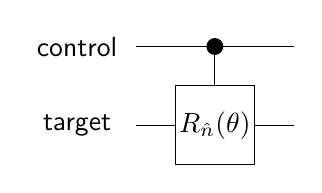
\begin{tikzpicture}[scale=.5] \node[draw=none] at (-3.5, 2) {control}; \node[draw=none] at (-3.5, 0) {target}; \draw (-2, 2) -- (2, 2); \draw[fill=black] (0, 2) circle (.2); \draw (0, 2) -- (0, 1); \draw (-2,0) -- (-1, 0); \draw (1, 0) -- (2, 0); \draw (-1,-1)--(-1,1)--(1,1)--(1,-1)--cycle; \node[draw=none] at (0, 0) {$R_{\hat{n}}(\theta)$}; \end{tikzpicture} } \]


\begin{DoxyParams}[1]{Parameters}
\mbox{\tt in,out}  & {\em multi\+Qubit} & object representing the set of all qubits \\
\hline
\mbox{\tt in}  & {\em control\+Qubit} & qubit with value 1 in the rotated states \\
\hline
\mbox{\tt in}  & {\em target\+Qubit} & qubit to rotate \\
\hline
\mbox{\tt in}  & {\em angle} & angle by which to rotate in radians \\
\hline
\mbox{\tt in}  & {\em axis} & vector around which to rotate (can be non-\/unit; will be normalised) \\
\hline
\end{DoxyParams}

\begin{DoxyExceptions}{Exceptions}
{\em exit\+With\+Error} & if either {\ttfamily control\+Qubit} or {\ttfamily target\+Qubit} are outside \mbox{[}0, {\ttfamily multi\+Qubit.\+num\+Qubits}) or are equal or if {\ttfamily axis} is the zero vector \\
\hline
\end{DoxyExceptions}


Definition at line 119 of file qubits.\+cpp.



References controlled\+Compact\+Unitary(), Complex\+::imag, Complex\+::real, Vector\+::x, Vector\+::y, and Vector\+::z.



Referenced by controlled\+Rotate\+X(), controlled\+Rotate\+Y(), and controlled\+Rotate\+Z().


\begin{DoxyCode}
119                                                                                                            
                         \{
120 
121     \textcolor{keywordtype}{double} mag = sqrt(pow(axis.\mbox{\hyperlink{structVector_aac7abe171ba4bada50ed72acba6259fc}{x}},2) + pow(axis.\mbox{\hyperlink{structVector_a375ca805d4c808a53d7c4e0c737ae3de}{y}},2) + pow(axis.\mbox{\hyperlink{structVector_ad4e863651be7d6b7e2b28cd7445a0ccf}{z}},2));
122     \mbox{\hyperlink{structVector}{Vector}} unitAxis = \{axis.\mbox{\hyperlink{structVector_aac7abe171ba4bada50ed72acba6259fc}{x}}/mag, axis.\mbox{\hyperlink{structVector_a375ca805d4c808a53d7c4e0c737ae3de}{y}}/mag, axis.\mbox{\hyperlink{structVector_ad4e863651be7d6b7e2b28cd7445a0ccf}{z}}/mag\};
123 
124     \mbox{\hyperlink{structComplex}{Complex}} alpha, beta;
125     alpha.\mbox{\hyperlink{structComplex_a479ad939835457595fcca3ca55c06283}{real}} = cos(angle/2.0);
126     alpha.\mbox{\hyperlink{structComplex_a1151948284b21c0052f203f23ab931d9}{imag}} = -sin(angle/2.0)*unitAxis.\mbox{\hyperlink{structVector_ad4e863651be7d6b7e2b28cd7445a0ccf}{z}};    
127     beta.\mbox{\hyperlink{structComplex_a479ad939835457595fcca3ca55c06283}{real}} = sin(angle/2.0)*unitAxis.\mbox{\hyperlink{structVector_a375ca805d4c808a53d7c4e0c737ae3de}{y}};
128     beta.\mbox{\hyperlink{structComplex_a1151948284b21c0052f203f23ab931d9}{imag}} = -sin(angle/2.0)*unitAxis.\mbox{\hyperlink{structVector_aac7abe171ba4bada50ed72acba6259fc}{x}};
129     \mbox{\hyperlink{qubits_8h_ab4812953bc457405b3aa05a4c2f64f4a}{controlledCompactUnitary}}(multiQubit, controlQubit, targetQubit, alpha, beta);
130 \}
\end{DoxyCode}
\mbox{\Hypertarget{qubits_8cpp_ac6923ac57e67d9a21096e06f6a9012f6}\label{qubits_8cpp_ac6923ac57e67d9a21096e06f6a9012f6}} 
\index{qubits.\+cpp@{qubits.\+cpp}!controlled\+RotateX@{controlled\+RotateX}}
\index{controlled\+RotateX@{controlled\+RotateX}!qubits.\+cpp@{qubits.\+cpp}}
\paragraph{\texorpdfstring{controlled\+Rotate\+X()}{controlledRotateX()}}
{\footnotesize\ttfamily void controlled\+RotateX (\begin{DoxyParamCaption}\item[{\mbox{\hyperlink{structMultiQubit}{Multi\+Qubit}}}]{multi\+Qubit,  }\item[{const int}]{control\+Qubit,  }\item[{const int}]{target\+Qubit,  }\item[{\mbox{\hyperlink{precision_8h_a4b654506f18b8bfd61ad2a29a7e38c25}{R\+E\+AL}}}]{angle }\end{DoxyParamCaption})}



Applies a controlled rotation by a given angle around the X-\/axis of the Bloch-\/sphere. 

The target qubit is rotated in states where the control qubit has value 1.

\[ \setlength{\fboxrule}{0.01pt} \fbox{ 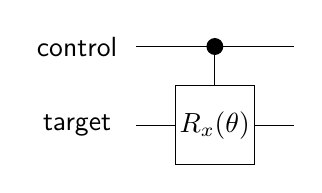
\begin{tikzpicture}[scale=.5] \node[draw=none] at (-3.5, 2) {control}; \node[draw=none] at (-3.5, 0) {target}; \draw (-2, 2) -- (2, 2); \draw[fill=black] (0, 2) circle (.2); \draw (0, 2) -- (0, 1); \draw (-2,0) -- (-1, 0); \draw (1, 0) -- (2, 0); \draw (-1,-1)--(-1,1)--(1,1)--(1,-1)--cycle; \node[draw=none] at (0, 0) {$R_x(\theta)$}; \end{tikzpicture} } \] ~\newline
 
\begin{DoxyParams}[1]{Parameters}
\mbox{\tt in,out}  & {\em multi\+Qubit} & object representing the set of all qubits \\
\hline
\mbox{\tt in}  & {\em control\+Qubit} & qubit which has value 1 in the rotated states \\
\hline
\mbox{\tt in}  & {\em tagret\+Qubit} & qubit to rotate \\
\hline
\mbox{\tt in}  & {\em angle} & angle by which to rotate the target qubit in radians \\
\hline
\end{DoxyParams}

\begin{DoxyExceptions}{Exceptions}
{\em exit\+With\+Error} & if either {\ttfamily control\+Qubit} or {\ttfamily target\+Qubit} are outside \mbox{[}0, {\ttfamily multi\+Qubit.\+num\+Qubits}) or are equal. \\
\hline
\end{DoxyExceptions}


Definition at line 132 of file qubits.\+cpp.



References controlled\+Rotate\+Around\+Axis().


\begin{DoxyCode}
132                                                                                                         \{
133 
134     \mbox{\hyperlink{structVector}{Vector}} unitAxis = \{1, 0, 0\};
135     \mbox{\hyperlink{qubits_8cpp_ad41f82b41149393a642391b67b3a287e}{controlledRotateAroundAxis}}(multiQubit, controlQubit, targetQubit, angle, 
      unitAxis);
136 \}
\end{DoxyCode}
\mbox{\Hypertarget{qubits_8cpp_a71e90a2f7292116338c062934f9d1202}\label{qubits_8cpp_a71e90a2f7292116338c062934f9d1202}} 
\index{qubits.\+cpp@{qubits.\+cpp}!controlled\+RotateY@{controlled\+RotateY}}
\index{controlled\+RotateY@{controlled\+RotateY}!qubits.\+cpp@{qubits.\+cpp}}
\paragraph{\texorpdfstring{controlled\+Rotate\+Y()}{controlledRotateY()}}
{\footnotesize\ttfamily void controlled\+RotateY (\begin{DoxyParamCaption}\item[{\mbox{\hyperlink{structMultiQubit}{Multi\+Qubit}}}]{multi\+Qubit,  }\item[{const int}]{control\+Qubit,  }\item[{const int}]{target\+Qubit,  }\item[{\mbox{\hyperlink{precision_8h_a4b654506f18b8bfd61ad2a29a7e38c25}{R\+E\+AL}}}]{angle }\end{DoxyParamCaption})}



Applies a controlled rotation by a given angle around the Y-\/axis of the Bloch-\/sphere. 

The target qubit is rotated in states where the control qubit has value 1.

\[ \setlength{\fboxrule}{0.01pt} \fbox{ 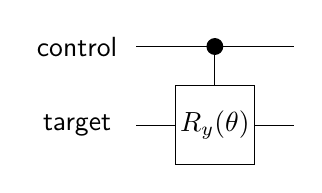
\begin{tikzpicture}[scale=.5] \node[draw=none] at (-3.5, 2) {control}; \node[draw=none] at (-3.5, 0) {target}; \draw (-2, 2) -- (2, 2); \draw[fill=black] (0, 2) circle (.2); \draw (0, 2) -- (0, 1); \draw (-2,0) -- (-1, 0); \draw (1, 0) -- (2, 0); \draw (-1,-1)--(-1,1)--(1,1)--(1,-1)--cycle; \node[draw=none] at (0, 0) {$R_y(\theta)$}; \end{tikzpicture} } \] ~\newline
 
\begin{DoxyParams}[1]{Parameters}
\mbox{\tt in,out}  & {\em multi\+Qubit} & object representing the set of all qubits \\
\hline
\mbox{\tt in}  & {\em control\+Qubit} & qubit which has value 1 in the rotated states \\
\hline
\mbox{\tt in}  & {\em tagret\+Qubit} & qubit to rotate \\
\hline
\mbox{\tt in}  & {\em angle} & angle by which to rotate the target qubit in radians \\
\hline
\end{DoxyParams}

\begin{DoxyExceptions}{Exceptions}
{\em exit\+With\+Error} & if either {\ttfamily control\+Qubit} or {\ttfamily target\+Qubit} are outside \mbox{[}0, {\ttfamily multi\+Qubit.\+num\+Qubits}) or are equal. \\
\hline
\end{DoxyExceptions}


Definition at line 138 of file qubits.\+cpp.



References controlled\+Rotate\+Around\+Axis().


\begin{DoxyCode}
138                                                                                                         \{
139 
140     \mbox{\hyperlink{structVector}{Vector}} unitAxis = \{0, 1, 0\};
141     \mbox{\hyperlink{qubits_8cpp_ad41f82b41149393a642391b67b3a287e}{controlledRotateAroundAxis}}(multiQubit, controlQubit, targetQubit, angle, 
      unitAxis);
142 \}
\end{DoxyCode}
\mbox{\Hypertarget{qubits_8cpp_a668e5d2634b02e98bc73675ccb11d61c}\label{qubits_8cpp_a668e5d2634b02e98bc73675ccb11d61c}} 
\index{qubits.\+cpp@{qubits.\+cpp}!controlled\+RotateZ@{controlled\+RotateZ}}
\index{controlled\+RotateZ@{controlled\+RotateZ}!qubits.\+cpp@{qubits.\+cpp}}
\paragraph{\texorpdfstring{controlled\+Rotate\+Z()}{controlledRotateZ()}}
{\footnotesize\ttfamily void controlled\+RotateZ (\begin{DoxyParamCaption}\item[{\mbox{\hyperlink{structMultiQubit}{Multi\+Qubit}}}]{multi\+Qubit,  }\item[{const int}]{control\+Qubit,  }\item[{const int}]{target\+Qubit,  }\item[{\mbox{\hyperlink{precision_8h_a4b654506f18b8bfd61ad2a29a7e38c25}{R\+E\+AL}}}]{angle }\end{DoxyParamCaption})}



Applies a controlled rotation by a given angle around the Z-\/axis of the Bloch-\/sphere. 

The target qubit is rotated in states where the control qubit has value 1.

\[ \setlength{\fboxrule}{0.01pt} \fbox{ 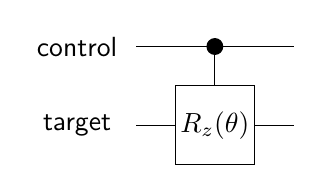
\begin{tikzpicture}[scale=.5] \node[draw=none] at (-3.5, 2) {control}; \node[draw=none] at (-3.5, 0) {target}; \draw (-2, 2) -- (2, 2); \draw[fill=black] (0, 2) circle (.2); \draw (0, 2) -- (0, 1); \draw (-2,0) -- (-1, 0); \draw (1, 0) -- (2, 0); \draw (-1,-1)--(-1,1)--(1,1)--(1,-1)--cycle; \node[draw=none] at (0, 0) {$R_z(\theta)$}; \end{tikzpicture} } \] ~\newline
 
\begin{DoxyParams}[1]{Parameters}
\mbox{\tt in,out}  & {\em multi\+Qubit} & object representing the set of all qubits \\
\hline
\mbox{\tt in}  & {\em control\+Qubit} & qubit which has value 1 in the rotated states \\
\hline
\mbox{\tt in}  & {\em tagret\+Qubit} & qubit to rotate \\
\hline
\mbox{\tt in}  & {\em angle} & angle by which to rotate the target qubit in radians \\
\hline
\end{DoxyParams}

\begin{DoxyExceptions}{Exceptions}
{\em exit\+With\+Error} & if either {\ttfamily control\+Qubit} or {\ttfamily target\+Qubit} are outside \mbox{[}0, {\ttfamily multi\+Qubit.\+num\+Qubits}) or are equal. \\
\hline
\end{DoxyExceptions}


Definition at line 144 of file qubits.\+cpp.



References controlled\+Rotate\+Around\+Axis().


\begin{DoxyCode}
144                                                                                                         \{
145 
146     \mbox{\hyperlink{structVector}{Vector}} unitAxis = \{0, 0, 1\};
147     \mbox{\hyperlink{qubits_8cpp_ad41f82b41149393a642391b67b3a287e}{controlledRotateAroundAxis}}(multiQubit, controlQubit, targetQubit, angle, 
      unitAxis);
148 \}
\end{DoxyCode}
\mbox{\Hypertarget{qubits_8cpp_ab76254cfde16f0808476649507a1a2fc}\label{qubits_8cpp_ab76254cfde16f0808476649507a1a2fc}} 
\index{qubits.\+cpp@{qubits.\+cpp}!hash\+String@{hash\+String}}
\index{hash\+String@{hash\+String}!qubits.\+cpp@{qubits.\+cpp}}
\paragraph{\texorpdfstring{hash\+String()}{hashString()}}
{\footnotesize\ttfamily unsigned long int hash\+String (\begin{DoxyParamCaption}\item[{char $\ast$}]{str }\end{DoxyParamCaption})}



Definition at line 235 of file qubits.\+cpp.



Referenced by Qu\+E\+S\+T\+Seed\+Random\+Default().


\begin{DoxyCode}
235                                        \{
236     \textcolor{keywordtype}{unsigned} \textcolor{keywordtype}{long} \textcolor{keywordtype}{int} hash = 5381;
237     \textcolor{keywordtype}{int} c;
238 
239     \textcolor{keywordflow}{while} ((c = *str++))
240         hash = ((hash << 5) + hash) + c; \textcolor{comment}{/* hash * 33 + c */}
241 
242     \textcolor{keywordflow}{return} hash;    
243 \}
\end{DoxyCode}
\mbox{\Hypertarget{qubits_8cpp_aedb5ef39da69e7895d714980dc621261}\label{qubits_8cpp_aedb5ef39da69e7895d714980dc621261}} 
\index{qubits.\+cpp@{qubits.\+cpp}!Qu\+E\+S\+T\+Seed\+Random@{Qu\+E\+S\+T\+Seed\+Random}}
\index{Qu\+E\+S\+T\+Seed\+Random@{Qu\+E\+S\+T\+Seed\+Random}!qubits.\+cpp@{qubits.\+cpp}}
\paragraph{\texorpdfstring{Qu\+E\+S\+T\+Seed\+Random()}{QuESTSeedRandom()}}
{\footnotesize\ttfamily void Qu\+E\+S\+T\+Seed\+Random (\begin{DoxyParamCaption}\item[{unsigned long int $\ast$}]{seed\+Array,  }\item[{int}]{num\+Seeds }\end{DoxyParamCaption})}



num\+Seeds $<$= 64 

Seed the Mersenne Twister used for random number generation in the Qu\+E\+ST environment with a user defined seed. 

Definition at line 228 of file qubits.\+cpp.



References init\+\_\+by\+\_\+array().


\begin{DoxyCode}
228                                                                 \{
229     \textcolor{comment}{// init MT random number generator with user defined list of seeds}
230     \textcolor{comment}{// for the MPI version, it is ok that all procs will get the same seed as random numbers will only be }
231     \textcolor{comment}{// used by the master process}
232     \mbox{\hyperlink{mt19937ar_8cpp_ac1283f9b1ed571332f5ffe53545ffc16}{init\_by\_array}}(seedArray, numSeeds); 
233 \}
\end{DoxyCode}
\mbox{\Hypertarget{qubits_8cpp_a30b2a5228b8a21419db8aa82fa5e3167}\label{qubits_8cpp_a30b2a5228b8a21419db8aa82fa5e3167}} 
\index{qubits.\+cpp@{qubits.\+cpp}!Qu\+E\+S\+T\+Seed\+Random\+Default@{Qu\+E\+S\+T\+Seed\+Random\+Default}}
\index{Qu\+E\+S\+T\+Seed\+Random\+Default@{Qu\+E\+S\+T\+Seed\+Random\+Default}!qubits.\+cpp@{qubits.\+cpp}}
\paragraph{\texorpdfstring{Qu\+E\+S\+T\+Seed\+Random\+Default()}{QuESTSeedRandomDefault()}}
{\footnotesize\ttfamily void Qu\+E\+S\+T\+Seed\+Random\+Default (\begin{DoxyParamCaption}\item[{void}]{ }\end{DoxyParamCaption})}



Seed the Mersenne Twister used for random number generation in the Qu\+E\+ST environment with an example defualt seed. 

This default seeding function uses the mt19937 init\+\_\+by\+\_\+array function with three keys -- time, pid and hostname. Subsequent calls to mt19937 genrand functions will use this seeding. For a multi process code, the same seed is given to all process, therefore this seeding is only appropriate to use for functions such as measure where all processes require the same random value.

For more information about the MT, see \href{http://www.math.sci.hiroshima-u.ac.jp/~m-mat/MT/MT2002/emt19937ar.html}{\tt http\+://www.\+math.\+sci.\+hiroshima-\/u.\+ac.\+jp/$\sim$m-\/mat/\+M\+T/\+M\+T2002/emt19937ar.\+html} 

Definition at line 203 of file qubits.\+cpp.



References hash\+String(), and init\+\_\+by\+\_\+array().


\begin{DoxyCode}
203                              \{
204     \textcolor{comment}{// init MT random number generator with three keys -- time, pid and a hash of hostname }
205     \textcolor{comment}{// for the MPI version, it is ok that all procs will get the same seed as random numbers will only be }
206     \textcolor{comment}{// used by the master process}
207 
208     \textcolor{keyword}{struct }timeval  tv;
209     gettimeofday(&tv, NULL);
210 
211     \textcolor{keywordtype}{double} time\_in\_mill = 
212         (tv.tv\_sec) * 1000 + (tv.tv\_usec) / 1000 ; \textcolor{comment}{// convert tv\_sec & tv\_usec to millisecond}
213 
214     \textcolor{keywordtype}{unsigned} \textcolor{keywordtype}{long} \textcolor{keywordtype}{int} pid = getpid();
215     \textcolor{keywordtype}{unsigned} \textcolor{keywordtype}{long} \textcolor{keywordtype}{int} msecs = (\textcolor{keywordtype}{unsigned} \textcolor{keywordtype}{long} int) time\_in\_mill;
216     \textcolor{keywordtype}{char} hostName[MAXHOSTNAMELEN+1];
217     gethostname(hostName, \textcolor{keyword}{sizeof}(hostName));
218     \textcolor{keywordtype}{unsigned} \textcolor{keywordtype}{long} \textcolor{keywordtype}{int} hostNameInt = \mbox{\hyperlink{qubits_8cpp_ab76254cfde16f0808476649507a1a2fc}{hashString}}(hostName);
219 
220     \textcolor{keywordtype}{unsigned} \textcolor{keywordtype}{long} \textcolor{keywordtype}{int} key[3];
221     key[0] = msecs; key[1] = pid; key[2] = hostNameInt;
222     \mbox{\hyperlink{mt19937ar_8cpp_ac1283f9b1ed571332f5ffe53545ffc16}{init\_by\_array}}(key, 3); 
223 \}
\end{DoxyCode}
\mbox{\Hypertarget{qubits_8cpp_aa5e77e0e64f3a4a3d3f5cc7382bffcd9}\label{qubits_8cpp_aa5e77e0e64f3a4a3d3f5cc7382bffcd9}} 
\index{qubits.\+cpp@{qubits.\+cpp}!report\+Multi\+Qubit\+Params@{report\+Multi\+Qubit\+Params}}
\index{report\+Multi\+Qubit\+Params@{report\+Multi\+Qubit\+Params}!qubits.\+cpp@{qubits.\+cpp}}
\paragraph{\texorpdfstring{report\+Multi\+Qubit\+Params()}{reportMultiQubitParams()}}
{\footnotesize\ttfamily void report\+Multi\+Qubit\+Params (\begin{DoxyParamCaption}\item[{\mbox{\hyperlink{structMultiQubit}{Multi\+Qubit}}}]{multi\+Qubit }\end{DoxyParamCaption})}



Report metainformation about a set of qubits\+: number of qubits, number of probability amplitudes. 


\begin{DoxyParams}[1]{Parameters}
\mbox{\tt in,out}  & {\em multi\+Qubit} & object representing the set of qubits \\
\hline
\mbox{\tt in}  & {\em env} & object representing the execution environment (local, multinode etc) \\
\hline
\end{DoxyParams}


Definition at line 77 of file qubits.\+cpp.



References Multi\+Qubit\+::chunk\+Id, Multi\+Qubit\+::num\+Chunks, and Multi\+Qubit\+::num\+Qubits.


\begin{DoxyCode}
77                                                   \{
78         \textcolor{keywordtype}{long} \textcolor{keywordtype}{long} \textcolor{keywordtype}{int} numAmps = 1L << multiQubit.\mbox{\hyperlink{structMultiQubit_ab5b9795bdc6fb5855e1974dcbbaeb36f}{numQubits}};
79         \textcolor{keywordtype}{long} \textcolor{keywordtype}{long} \textcolor{keywordtype}{int} numAmpsPerRank = numAmps/multiQubit.\mbox{\hyperlink{structMultiQubit_acd43f2f57991709c9e94f73662c972b2}{numChunks}};
80         \textcolor{keywordflow}{if} (multiQubit.\mbox{\hyperlink{structMultiQubit_ab10c88249fa3825d6227ceec01d37e37}{chunkId}}==0)\{
81                 printf(\textcolor{stringliteral}{"QUBITS:\(\backslash\)n"});
82                 printf(\textcolor{stringliteral}{"Number of qubits is %d.\(\backslash\)n"}, multiQubit.\mbox{\hyperlink{structMultiQubit_ab5b9795bdc6fb5855e1974dcbbaeb36f}{numQubits}});
83                 printf(\textcolor{stringliteral}{"Number of amps is %lld.\(\backslash\)n"}, numAmps);
84                 printf(\textcolor{stringliteral}{"Number of amps per rank is %lld.\(\backslash\)n"}, numAmpsPerRank);
85     \}
86 \}
\end{DoxyCode}
\mbox{\Hypertarget{qubits_8cpp_a96f4de9ce7fefc7680a44d601fc3d894}\label{qubits_8cpp_a96f4de9ce7fefc7680a44d601fc3d894}} 
\index{qubits.\+cpp@{qubits.\+cpp}!report\+State@{report\+State}}
\index{report\+State@{report\+State}!qubits.\+cpp@{qubits.\+cpp}}
\paragraph{\texorpdfstring{report\+State()}{reportState()}}
{\footnotesize\ttfamily void report\+State (\begin{DoxyParamCaption}\item[{\mbox{\hyperlink{structMultiQubit}{Multi\+Qubit}}}]{multi\+Qubit }\end{DoxyParamCaption})}



Print the current state vector of probability amplitudes for a set of qubits to file. 

File format\+: \begin{DoxyVerb}real, imag
realComponent1, imagComponent1
realComponent2, imagComponent2
...
realComponentN, imagComponentN
\end{DoxyVerb}


File naming convention\+:

For each node that the program runs on, a file \textquotesingle{}state\+\_\+rank\+\_\+\mbox{[}node\+\_\+rank\mbox{]}.csv\textquotesingle{} is generated. If there is more than one node, ranks after the first do not include the header \begin{DoxyVerb}real, imag
\end{DoxyVerb}
 so that files are easier to combine. 
\begin{DoxyParams}[1]{Parameters}
\mbox{\tt in,out}  & {\em multi\+Qubit} & object representing the set of qubits \\
\hline
\end{DoxyParams}


Definition at line 59 of file qubits.\+cpp.



References Multi\+Qubit\+::chunk\+Id, Complex\+Array\+::imag, Multi\+Qubit\+::num\+Amps, Complex\+Array\+::real, and Multi\+Qubit\+::state\+Vec.


\begin{DoxyCode}
59                                        \{
60         FILE *state;
61         \textcolor{keywordtype}{char} filename[100];
62         \textcolor{keywordtype}{long} \textcolor{keywordtype}{long} \textcolor{keywordtype}{int} index;
63         sprintf(filename, \textcolor{stringliteral}{"state\_rank\_%d.csv"}, multiQubit.\mbox{\hyperlink{structMultiQubit_ab10c88249fa3825d6227ceec01d37e37}{chunkId}});
64         state = fopen(filename, \textcolor{stringliteral}{"w"});
65         \textcolor{keywordflow}{if} (multiQubit.\mbox{\hyperlink{structMultiQubit_ab10c88249fa3825d6227ceec01d37e37}{chunkId}}==0) fprintf(state, \textcolor{stringliteral}{"real, imag\(\backslash\)n"});
66 
67         \textcolor{keywordflow}{for}(index=0; index<multiQubit.\mbox{\hyperlink{structMultiQubit_ae16f47d8b725c914fb7f66b6498d79db}{numAmps}}; index++)\{
68                 fprintf(state, \textcolor{stringliteral}{"%.12f, %.12f\(\backslash\)n"}, multiQubit.\mbox{\hyperlink{structMultiQubit_a45483190d6b01ef6b2f98f2bec9ab94f}{stateVec}}.
      \mbox{\hyperlink{structComplexArray_a4195cac6c784ea1b6271f1c7dba1548a}{real}}[index], multiQubit.\mbox{\hyperlink{structMultiQubit_a45483190d6b01ef6b2f98f2bec9ab94f}{stateVec}}.\mbox{\hyperlink{structComplexArray_a79dde47c7ae530c79cebfdf57b225968}{imag}}[index]);
69         \}
70         fclose(state);
71 \}
\end{DoxyCode}
\mbox{\Hypertarget{qubits_8cpp_a8810423457803005fecd415f4299f40d}\label{qubits_8cpp_a8810423457803005fecd415f4299f40d}} 
\index{qubits.\+cpp@{qubits.\+cpp}!rotate\+Around\+Axis@{rotate\+Around\+Axis}}
\index{rotate\+Around\+Axis@{rotate\+Around\+Axis}!qubits.\+cpp@{qubits.\+cpp}}
\paragraph{\texorpdfstring{rotate\+Around\+Axis()}{rotateAroundAxis()}}
{\footnotesize\ttfamily void rotate\+Around\+Axis (\begin{DoxyParamCaption}\item[{\mbox{\hyperlink{structMultiQubit}{Multi\+Qubit}}}]{multi\+Qubit,  }\item[{const int}]{rot\+Qubit,  }\item[{\mbox{\hyperlink{precision_8h_a4b654506f18b8bfd61ad2a29a7e38c25}{R\+E\+AL}}}]{angle,  }\item[{\mbox{\hyperlink{structVector}{Vector}}}]{unit\+Axis }\end{DoxyParamCaption})}



Rotate a single qubit by a given angle around a given vector on the Bloch-\/sphere. 


\begin{DoxyItemize}
\item The vector must not be zero (else an error is thrown), but needn\textquotesingle{}t be unit magnitude.
\end{DoxyItemize}


\begin{DoxyParams}[1]{Parameters}
\mbox{\tt in,out}  & {\em multi\+Qubit} & object representing the set of all qubits \\
\hline
\mbox{\tt in}  & {\em rot\+Qubit} & qubit to rotate \\
\hline
\mbox{\tt in}  & {\em angle} & angle by which to rotate in radians \\
\hline
\mbox{\tt in}  & {\em axis} & vector around which to rotate \\
\hline
\end{DoxyParams}

\begin{DoxyExceptions}{Exceptions}
{\em exit\+With\+Error} & if {\ttfamily rot\+Qubit} is outside \mbox{[}0, {\ttfamily multi\+Qubit.\+num\+Qubits}), or if {\ttfamily axis} is the zero vector \\
\hline
\end{DoxyExceptions}


Definition at line 88 of file qubits.\+cpp.



References compact\+Unitary(), Complex\+::imag, Complex\+::real, Vector\+::x, Vector\+::y, and Vector\+::z.



Referenced by rotate\+X(), rotate\+Y(), and rotate\+Z().


\begin{DoxyCode}
88                                                                                          \{
89 
90     \textcolor{keywordtype}{double} mag = sqrt(pow(axis.\mbox{\hyperlink{structVector_aac7abe171ba4bada50ed72acba6259fc}{x}},2) + pow(axis.\mbox{\hyperlink{structVector_a375ca805d4c808a53d7c4e0c737ae3de}{y}},2) + pow(axis.\mbox{\hyperlink{structVector_ad4e863651be7d6b7e2b28cd7445a0ccf}{z}},2));
91     \mbox{\hyperlink{structVector}{Vector}} unitAxis = \{axis.\mbox{\hyperlink{structVector_aac7abe171ba4bada50ed72acba6259fc}{x}}/mag, axis.\mbox{\hyperlink{structVector_a375ca805d4c808a53d7c4e0c737ae3de}{y}}/mag, axis.\mbox{\hyperlink{structVector_ad4e863651be7d6b7e2b28cd7445a0ccf}{z}}/mag\};
92 
93     \mbox{\hyperlink{structComplex}{Complex}} alpha, beta;
94     alpha.\mbox{\hyperlink{structComplex_a479ad939835457595fcca3ca55c06283}{real}} = cos(angle/2.0);
95     alpha.\mbox{\hyperlink{structComplex_a1151948284b21c0052f203f23ab931d9}{imag}} = -sin(angle/2.0)*unitAxis.\mbox{\hyperlink{structVector_ad4e863651be7d6b7e2b28cd7445a0ccf}{z}};    
96     beta.\mbox{\hyperlink{structComplex_a479ad939835457595fcca3ca55c06283}{real}} = sin(angle/2.0)*unitAxis.\mbox{\hyperlink{structVector_a375ca805d4c808a53d7c4e0c737ae3de}{y}};
97     beta.\mbox{\hyperlink{structComplex_a1151948284b21c0052f203f23ab931d9}{imag}} = -sin(angle/2.0)*unitAxis.\mbox{\hyperlink{structVector_aac7abe171ba4bada50ed72acba6259fc}{x}};
98     \mbox{\hyperlink{qubits_8h_ad13ae1902276195d0df106116e032aff}{compactUnitary}}(multiQubit, rotQubit, alpha, beta);
99 \}
\end{DoxyCode}
\mbox{\Hypertarget{qubits_8cpp_a6cc7fa705a2f2e6b486b49c5589d5df5}\label{qubits_8cpp_a6cc7fa705a2f2e6b486b49c5589d5df5}} 
\index{qubits.\+cpp@{qubits.\+cpp}!rotateX@{rotateX}}
\index{rotateX@{rotateX}!qubits.\+cpp@{qubits.\+cpp}}
\paragraph{\texorpdfstring{rotate\+X()}{rotateX()}}
{\footnotesize\ttfamily void rotateX (\begin{DoxyParamCaption}\item[{\mbox{\hyperlink{structMultiQubit}{Multi\+Qubit}}}]{multi\+Qubit,  }\item[{const int}]{rot\+Qubit,  }\item[{\mbox{\hyperlink{precision_8h_a4b654506f18b8bfd61ad2a29a7e38c25}{R\+E\+AL}}}]{angle }\end{DoxyParamCaption})}



Rotate a single qubit by a given angle around the X-\/axis of the Bloch-\/sphere. 

For angle $\theta$, applies \[ \begin{pmatrix} \cos\theta/2 & -i \sin \theta/2\\ -i \sin \theta/2 & \cos \theta/2 \end{pmatrix} \]

\[ \setlength{\fboxrule}{0.01pt} \fbox{ 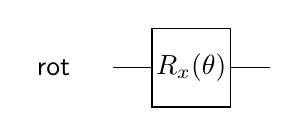
\begin{tikzpicture}[scale=.5] \node[draw=none] at (-3.5, 0) {rot}; \draw (-2,0) -- (-1, 0); \draw (1, 0) -- (2, 0); \draw (-1,-1)--(-1,1)--(1,1)--(1,-1)--cycle; \node[draw=none] at (0, 0) {$R_x(\theta)$}; \end{tikzpicture} } \]


\begin{DoxyParams}[1]{Parameters}
\mbox{\tt in,out}  & {\em multi\+Qubit} & object representing the set of all qubits \\
\hline
\mbox{\tt in}  & {\em rot\+Qubit} & qubit to rotate \\
\hline
\mbox{\tt in}  & {\em angle} & angle by which to rotate in radians \\
\hline
\end{DoxyParams}

\begin{DoxyExceptions}{Exceptions}
{\em exit\+With\+Error} & if {\ttfamily rot\+Qubit} is outside \mbox{[}0, {\ttfamily multi\+Qubit.\+num\+Qubits}). \\
\hline
\end{DoxyExceptions}


Definition at line 101 of file qubits.\+cpp.



References rotate\+Around\+Axis().


\begin{DoxyCode}
101                                                                    \{
102 
103     \mbox{\hyperlink{structVector}{Vector}} unitAxis = \{1, 0, 0\};
104     \mbox{\hyperlink{qubits_8cpp_a8810423457803005fecd415f4299f40d}{rotateAroundAxis}}(multiQubit, rotQubit, angle, unitAxis);
105 \}
\end{DoxyCode}
\mbox{\Hypertarget{qubits_8cpp_ace0d3592d38a990e81a434c4e9681500}\label{qubits_8cpp_ace0d3592d38a990e81a434c4e9681500}} 
\index{qubits.\+cpp@{qubits.\+cpp}!rotateY@{rotateY}}
\index{rotateY@{rotateY}!qubits.\+cpp@{qubits.\+cpp}}
\paragraph{\texorpdfstring{rotate\+Y()}{rotateY()}}
{\footnotesize\ttfamily void rotateY (\begin{DoxyParamCaption}\item[{\mbox{\hyperlink{structMultiQubit}{Multi\+Qubit}}}]{multi\+Qubit,  }\item[{const int}]{rot\+Qubit,  }\item[{\mbox{\hyperlink{precision_8h_a4b654506f18b8bfd61ad2a29a7e38c25}{R\+E\+AL}}}]{angle }\end{DoxyParamCaption})}



Rotate a single qubit by a given angle around the Y-\/axis of the Bloch-\/sphere. 

For angle $\theta$, applies \[ \begin{pmatrix} \cos\theta/2 & \sin \theta/2\\ \sin \theta/2 & \cos \theta/2 \end{pmatrix} \] ~\newline
 \[ \setlength{\fboxrule}{0.01pt} \fbox{ 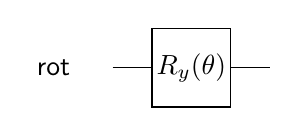
\begin{tikzpicture}[scale=.5] \node[draw=none] at (-3.5, 0) {rot}; \draw (-2,0) -- (-1, 0); \draw (1, 0) -- (2, 0); \draw (-1,-1)--(-1,1)--(1,1)--(1,-1)--cycle; \node[draw=none] at (0, 0) {$R_y(\theta)$}; \end{tikzpicture} } \]


\begin{DoxyParams}[1]{Parameters}
\mbox{\tt in,out}  & {\em multi\+Qubit} & object representing the set of all qubits \\
\hline
\mbox{\tt in}  & {\em rot\+Qubit} & qubit to rotate \\
\hline
\mbox{\tt in}  & {\em angle} & angle by which to rotate in radians \\
\hline
\end{DoxyParams}

\begin{DoxyExceptions}{Exceptions}
{\em exit\+With\+Error} & if {\ttfamily rot\+Qubit} is outside \mbox{[}0, {\ttfamily multi\+Qubit.\+num\+Qubits}). \\
\hline
\end{DoxyExceptions}


Definition at line 107 of file qubits.\+cpp.



References rotate\+Around\+Axis().


\begin{DoxyCode}
107                                                                    \{
108 
109     \mbox{\hyperlink{structVector}{Vector}} unitAxis = \{0, 1, 0\};
110     \mbox{\hyperlink{qubits_8cpp_a8810423457803005fecd415f4299f40d}{rotateAroundAxis}}(multiQubit, rotQubit, angle, unitAxis);
111 \}
\end{DoxyCode}
\mbox{\Hypertarget{qubits_8cpp_abd621412ad30c1b034f4ce153c4afe10}\label{qubits_8cpp_abd621412ad30c1b034f4ce153c4afe10}} 
\index{qubits.\+cpp@{qubits.\+cpp}!rotateZ@{rotateZ}}
\index{rotateZ@{rotateZ}!qubits.\+cpp@{qubits.\+cpp}}
\paragraph{\texorpdfstring{rotate\+Z()}{rotateZ()}}
{\footnotesize\ttfamily void rotateZ (\begin{DoxyParamCaption}\item[{\mbox{\hyperlink{structMultiQubit}{Multi\+Qubit}}}]{multi\+Qubit,  }\item[{const int}]{rot\+Qubit,  }\item[{\mbox{\hyperlink{precision_8h_a4b654506f18b8bfd61ad2a29a7e38c25}{R\+E\+AL}}}]{angle }\end{DoxyParamCaption})}



Rotate a single qubit by a given angle around the Z-\/axis of the Bloch-\/sphere (also known as a phase shift gate). 

For angle $\theta$, applies \[ \begin{pmatrix} \exp(-i \theta/2) & 0 \\ 0 & \exp(i \theta/2) \end{pmatrix} \]

\[ \setlength{\fboxrule}{0.01pt} \fbox{ 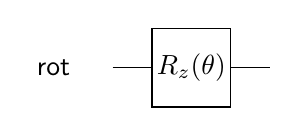
\begin{tikzpicture}[scale=.5] \node[draw=none] at (-3.5, 0) {rot}; \draw (-2,0) -- (-1, 0); \draw (1, 0) -- (2, 0); \draw (-1,-1)--(-1,1)--(1,1)--(1,-1)--cycle; \node[draw=none] at (0, 0) {$R_z(\theta)$}; \end{tikzpicture} } \]


\begin{DoxyParams}[1]{Parameters}
\mbox{\tt in,out}  & {\em multi\+Qubit} & object representing the set of all qubits \\
\hline
\mbox{\tt in}  & {\em rot\+Qubit} & qubit to rotate \\
\hline
\mbox{\tt in}  & {\em angle} & angle by which to rotate in radians \\
\hline
\end{DoxyParams}

\begin{DoxyExceptions}{Exceptions}
{\em exit\+With\+Error} & if {\ttfamily rot\+Qubit} is outside \mbox{[}0, {\ttfamily multi\+Qubit.\+num\+Qubits}). \\
\hline
\end{DoxyExceptions}


Definition at line 113 of file qubits.\+cpp.



References rotate\+Around\+Axis().


\begin{DoxyCode}
113                                                                    \{
114 
115     \mbox{\hyperlink{structVector}{Vector}} unitAxis = \{0, 0, 1\};
116     \mbox{\hyperlink{qubits_8cpp_a8810423457803005fecd415f4299f40d}{rotateAroundAxis}}(multiQubit, rotQubit, angle, unitAxis);
117 \}
\end{DoxyCode}
\mbox{\Hypertarget{qubits_8cpp_adda6c47876a7676488ed0565a19eaa65}\label{qubits_8cpp_adda6c47876a7676488ed0565a19eaa65}} 
\index{qubits.\+cpp@{qubits.\+cpp}!s\+Gate@{s\+Gate}}
\index{s\+Gate@{s\+Gate}!qubits.\+cpp@{qubits.\+cpp}}
\paragraph{\texorpdfstring{s\+Gate()}{sGate()}}
{\footnotesize\ttfamily void s\+Gate (\begin{DoxyParamCaption}\item[{\mbox{\hyperlink{structMultiQubit}{Multi\+Qubit}}}]{multi\+Qubit,  }\item[{const int}]{target\+Qubit }\end{DoxyParamCaption})}



Apply the single-\/qubit S gate. 

This is a rotation of $\pi/2$ around the Z-\/axis on the Bloch sphere, or the unitary\+: \[ \begin{pmatrix} 1 & 0 \\ 0 & i \end{pmatrix} \]

\[ \setlength{\fboxrule}{0.01pt} \fbox{ 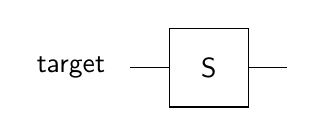
\begin{tikzpicture}[scale=.5] \node[draw=none] at (-3.5, 0) {target}; \draw (-2,0) -- (-1, 0); \draw (1, 0) -- (2, 0); \draw (-1,-1)--(-1,1)--(1,1)--(1,-1)--cycle; \node[draw=none] at (0, 0) {S}; \end{tikzpicture} } \]


\begin{DoxyParams}[1]{Parameters}
\mbox{\tt in,out}  & {\em multi\+Qubit} & object representing the set of all qubits \\
\hline
\mbox{\tt in}  & {\em target\+Qubit} & qubit to operate upon \\
\hline
\end{DoxyParams}

\begin{DoxyExceptions}{Exceptions}
{\em exit\+With\+Error} & if {\ttfamily target\+Qubit} is outside \mbox{[}0, {\ttfamily multi\+Qubit.\+num\+Qubits}) \\
\hline
\end{DoxyExceptions}


Definition at line 155 of file qubits.\+cpp.



References phase\+Gate(), and S\+\_\+\+G\+A\+TE.


\begin{DoxyCode}
156 \{
157     \mbox{\hyperlink{qubits__internal_8h_aae7a8a7f1ccbddb7f76b6c52b746bb43}{phaseGate}}(multiQubit, targetQubit, \mbox{\hyperlink{qubits_8h_a5739021c733cecc49647956b2f7338eaa06e60f80fa80cce271793d6d31bcc21f}{S\_GATE}});
158 \} 
\end{DoxyCode}
\mbox{\Hypertarget{qubits_8cpp_aebaab86326779de55d335cfea3efde8f}\label{qubits_8cpp_aebaab86326779de55d335cfea3efde8f}} 
\index{qubits.\+cpp@{qubits.\+cpp}!sigmaZ@{sigmaZ}}
\index{sigmaZ@{sigmaZ}!qubits.\+cpp@{qubits.\+cpp}}
\paragraph{\texorpdfstring{sigma\+Z()}{sigmaZ()}}
{\footnotesize\ttfamily void sigmaZ (\begin{DoxyParamCaption}\item[{\mbox{\hyperlink{structMultiQubit}{Multi\+Qubit}}}]{multi\+Qubit,  }\item[{const int}]{target\+Qubit }\end{DoxyParamCaption})}



Apply the single-\/qubit sigma-\/Z (also known as the Z, Pauli-\/Z or phase-\/flip) gate. 

This is a rotation of $\pi$ around the Z-\/axis (a phase shift) on the Bloch sphere. I.\+e. \[ \begin{pmatrix} 1 & 0 \\ 0 & -1 \end{pmatrix} \] ~\newline
 \[ \setlength{\fboxrule}{0.01pt} \fbox{ 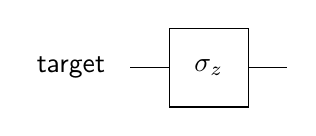
\begin{tikzpicture}[scale=.5] \node[draw=none] at (-3.5, 0) {target}; \draw (-2,0) -- (-1, 0); \draw (1, 0) -- (2, 0); \draw (-1,-1)--(-1,1)--(1,1)--(1,-1)--cycle; \node[draw=none] at (0, 0) {$\sigma_z$}; \end{tikzpicture} } \] ~\newline
 
\begin{DoxyParams}[1]{Parameters}
\mbox{\tt in,out}  & {\em multi\+Qubit} & object representing the set of all qubits \\
\hline
\mbox{\tt in}  & {\em target\+Qubit} & qubit to operate on \\
\hline
\end{DoxyParams}

\begin{DoxyExceptions}{Exceptions}
{\em exit\+With\+Error} & if {\ttfamily target\+Qubit} is outside \mbox{[}0, {\ttfamily multi\+Qubit.\+num\+Qubits}). \\
\hline
\end{DoxyExceptions}


Definition at line 150 of file qubits.\+cpp.



References phase\+Gate(), and S\+I\+G\+M\+A\+\_\+Z.


\begin{DoxyCode}
151 \{
152     \mbox{\hyperlink{qubits__internal_8h_aae7a8a7f1ccbddb7f76b6c52b746bb43}{phaseGate}}(multiQubit, targetQubit, \mbox{\hyperlink{qubits_8h_a5739021c733cecc49647956b2f7338eaa754922d1e1846a1961ff2bf163483dac}{SIGMA\_Z}});
153 \}
\end{DoxyCode}
\mbox{\Hypertarget{qubits_8cpp_af764ea63a2e870098f4e1ce08562942e}\label{qubits_8cpp_af764ea63a2e870098f4e1ce08562942e}} 
\index{qubits.\+cpp@{qubits.\+cpp}!t\+Gate@{t\+Gate}}
\index{t\+Gate@{t\+Gate}!qubits.\+cpp@{qubits.\+cpp}}
\paragraph{\texorpdfstring{t\+Gate()}{tGate()}}
{\footnotesize\ttfamily void t\+Gate (\begin{DoxyParamCaption}\item[{\mbox{\hyperlink{structMultiQubit}{Multi\+Qubit}}}]{multi\+Qubit,  }\item[{const int}]{target\+Qubit }\end{DoxyParamCaption})}



Apply the single-\/qubit T gate. 

This is a rotation of $\pi/4$ around the Z-\/axis on the Bloch sphere, or the unitary\+: \[ \begin{pmatrix} 1 & 0 \\ 0 & \exp\left(i \frac{\pi}{4}\right) \end{pmatrix} \]

\[ \setlength{\fboxrule}{0.01pt} \fbox{ 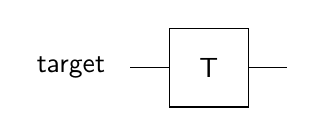
\begin{tikzpicture}[scale=.5] \node[draw=none] at (-3.5, 0) {target}; \draw (-2,0) -- (-1, 0); \draw (1, 0) -- (2, 0); \draw (-1,-1)--(-1,1)--(1,1)--(1,-1)--cycle; \node[draw=none] at (0, 0) {T}; \end{tikzpicture} } \]


\begin{DoxyParams}[1]{Parameters}
\mbox{\tt in,out}  & {\em multi\+Qubit} & object representing the set of all qubits \\
\hline
\mbox{\tt in}  & {\em target\+Qubit} & qubit to operate upon \\
\hline
\end{DoxyParams}

\begin{DoxyExceptions}{Exceptions}
{\em exit\+With\+Error} & if {\ttfamily target\+Qubit} is outside \mbox{[}0, {\ttfamily multi\+Qubit.\+num\+Qubits}) \\
\hline
\end{DoxyExceptions}


Definition at line 160 of file qubits.\+cpp.



References phase\+Gate(), and T\+\_\+\+G\+A\+TE.


\begin{DoxyCode}
161 \{
162     \mbox{\hyperlink{qubits__internal_8h_aae7a8a7f1ccbddb7f76b6c52b746bb43}{phaseGate}}(multiQubit, targetQubit, \mbox{\hyperlink{qubits_8h_a5739021c733cecc49647956b2f7338eaa614d07d597a8e320cc556bc0e652e4ab}{T\_GATE}});
163 \}
\end{DoxyCode}
\mbox{\Hypertarget{qubits_8cpp_ae2b2c14a07dd7d50ff86032a3ca101d7}\label{qubits_8cpp_ae2b2c14a07dd7d50ff86032a3ca101d7}} 
\index{qubits.\+cpp@{qubits.\+cpp}!validate\+Alpha\+Beta@{validate\+Alpha\+Beta}}
\index{validate\+Alpha\+Beta@{validate\+Alpha\+Beta}!qubits.\+cpp@{qubits.\+cpp}}
\paragraph{\texorpdfstring{validate\+Alpha\+Beta()}{validateAlphaBeta()}}
{\footnotesize\ttfamily int validate\+Alpha\+Beta (\begin{DoxyParamCaption}\item[{\mbox{\hyperlink{structComplex}{Complex}}}]{alpha,  }\item[{\mbox{\hyperlink{structComplex}{Complex}}}]{beta }\end{DoxyParamCaption})}



Definition at line 190 of file qubits.\+cpp.



References Complex\+::imag, Complex\+::real, and R\+E\+A\+L\+\_\+\+E\+PS.


\begin{DoxyCode}
190                                                   \{
191     \textcolor{keywordflow}{if} ( fabs(alpha.\mbox{\hyperlink{structComplex_a479ad939835457595fcca3ca55c06283}{real}}*alpha.\mbox{\hyperlink{structComplex_a479ad939835457595fcca3ca55c06283}{real}} 
192         + alpha.\mbox{\hyperlink{structComplex_a1151948284b21c0052f203f23ab931d9}{imag}}*alpha.\mbox{\hyperlink{structComplex_a1151948284b21c0052f203f23ab931d9}{imag}}
193         + beta.\mbox{\hyperlink{structComplex_a479ad939835457595fcca3ca55c06283}{real}}*beta.\mbox{\hyperlink{structComplex_a479ad939835457595fcca3ca55c06283}{real}} 
194         + beta.\mbox{\hyperlink{structComplex_a1151948284b21c0052f203f23ab931d9}{imag}}*beta.\mbox{\hyperlink{structComplex_a1151948284b21c0052f203f23ab931d9}{imag}} - 1) > \mbox{\hyperlink{precision_8h_aebb5e6716e06431296af4d1a71744dec}{REAL\_EPS}} ) \textcolor{keywordflow}{return} 0;
195     \textcolor{keywordflow}{else} \textcolor{keywordflow}{return} 1;
196 \}
\end{DoxyCode}
\mbox{\Hypertarget{qubits_8cpp_ae4fea133d1a8f09ff8da03038100adb2}\label{qubits_8cpp_ae4fea133d1a8f09ff8da03038100adb2}} 
\index{qubits.\+cpp@{qubits.\+cpp}!validate\+Matrix\+Is\+Unitary@{validate\+Matrix\+Is\+Unitary}}
\index{validate\+Matrix\+Is\+Unitary@{validate\+Matrix\+Is\+Unitary}!qubits.\+cpp@{qubits.\+cpp}}
\paragraph{\texorpdfstring{validate\+Matrix\+Is\+Unitary()}{validateMatrixIsUnitary()}}
{\footnotesize\ttfamily int validate\+Matrix\+Is\+Unitary (\begin{DoxyParamCaption}\item[{\mbox{\hyperlink{structComplexMatrix2}{Complex\+Matrix2}}}]{u }\end{DoxyParamCaption})}



Definition at line 165 of file qubits.\+cpp.



References Complex\+::imag, Complex\+Matrix2\+::r0c0, Complex\+Matrix2\+::r0c1, Complex\+Matrix2\+::r1c0, Complex\+Matrix2\+::r1c1, Complex\+::real, and R\+E\+A\+L\+\_\+\+E\+PS.


\begin{DoxyCode}
165                                              \{
166 
167     \textcolor{keywordflow}{if} ( fabs(u.\mbox{\hyperlink{structComplexMatrix2_ae72b4458233b077a636beee1892e81ff}{r0c0}}.\mbox{\hyperlink{structComplex_a479ad939835457595fcca3ca55c06283}{real}}*u.\mbox{\hyperlink{structComplexMatrix2_ae72b4458233b077a636beee1892e81ff}{r0c0}}.\mbox{\hyperlink{structComplex_a479ad939835457595fcca3ca55c06283}{real}} 
168         + u.\mbox{\hyperlink{structComplexMatrix2_ae72b4458233b077a636beee1892e81ff}{r0c0}}.\mbox{\hyperlink{structComplex_a1151948284b21c0052f203f23ab931d9}{imag}}*u.\mbox{\hyperlink{structComplexMatrix2_ae72b4458233b077a636beee1892e81ff}{r0c0}}.\mbox{\hyperlink{structComplex_a1151948284b21c0052f203f23ab931d9}{imag}}
169         + u.\mbox{\hyperlink{structComplexMatrix2_ab98282015ed2065e53fbc9638e2583ab}{r1c0}}.\mbox{\hyperlink{structComplex_a479ad939835457595fcca3ca55c06283}{real}}*u.\mbox{\hyperlink{structComplexMatrix2_ab98282015ed2065e53fbc9638e2583ab}{r1c0}}.\mbox{\hyperlink{structComplex_a479ad939835457595fcca3ca55c06283}{real}}
170         + u.\mbox{\hyperlink{structComplexMatrix2_ab98282015ed2065e53fbc9638e2583ab}{r1c0}}.\mbox{\hyperlink{structComplex_a1151948284b21c0052f203f23ab931d9}{imag}}*u.\mbox{\hyperlink{structComplexMatrix2_ab98282015ed2065e53fbc9638e2583ab}{r1c0}}.\mbox{\hyperlink{structComplex_a1151948284b21c0052f203f23ab931d9}{imag}} - 1) > \mbox{\hyperlink{precision_8h_aebb5e6716e06431296af4d1a71744dec}{REAL\_EPS}} ) \textcolor{keywordflow}{return} 0;
171     \textcolor{comment}{// check}
172     \textcolor{keywordflow}{if} ( fabs(u.\mbox{\hyperlink{structComplexMatrix2_a0f3932f055a8b05cef361bce25d51172}{r0c1}}.\mbox{\hyperlink{structComplex_a479ad939835457595fcca3ca55c06283}{real}}*u.\mbox{\hyperlink{structComplexMatrix2_a0f3932f055a8b05cef361bce25d51172}{r0c1}}.\mbox{\hyperlink{structComplex_a479ad939835457595fcca3ca55c06283}{real}} 
173         + u.\mbox{\hyperlink{structComplexMatrix2_a0f3932f055a8b05cef361bce25d51172}{r0c1}}.\mbox{\hyperlink{structComplex_a1151948284b21c0052f203f23ab931d9}{imag}}*u.\mbox{\hyperlink{structComplexMatrix2_a0f3932f055a8b05cef361bce25d51172}{r0c1}}.\mbox{\hyperlink{structComplex_a1151948284b21c0052f203f23ab931d9}{imag}}
174         + u.\mbox{\hyperlink{structComplexMatrix2_a763007c3070802373549ba0350f83c8a}{r1c1}}.\mbox{\hyperlink{structComplex_a479ad939835457595fcca3ca55c06283}{real}}*u.\mbox{\hyperlink{structComplexMatrix2_a763007c3070802373549ba0350f83c8a}{r1c1}}.\mbox{\hyperlink{structComplex_a479ad939835457595fcca3ca55c06283}{real}}
175         + u.\mbox{\hyperlink{structComplexMatrix2_a763007c3070802373549ba0350f83c8a}{r1c1}}.\mbox{\hyperlink{structComplex_a1151948284b21c0052f203f23ab931d9}{imag}}*u.\mbox{\hyperlink{structComplexMatrix2_a763007c3070802373549ba0350f83c8a}{r1c1}}.\mbox{\hyperlink{structComplex_a1151948284b21c0052f203f23ab931d9}{imag}} - 1) > \mbox{\hyperlink{precision_8h_aebb5e6716e06431296af4d1a71744dec}{REAL\_EPS}} ) \textcolor{keywordflow}{return} 0;
176 
177     \textcolor{keywordflow}{if} ( fabs(u.\mbox{\hyperlink{structComplexMatrix2_ae72b4458233b077a636beee1892e81ff}{r0c0}}.\mbox{\hyperlink{structComplex_a479ad939835457595fcca3ca55c06283}{real}}*u.\mbox{\hyperlink{structComplexMatrix2_a0f3932f055a8b05cef361bce25d51172}{r0c1}}.\mbox{\hyperlink{structComplex_a479ad939835457595fcca3ca55c06283}{real}} 
178         + u.\mbox{\hyperlink{structComplexMatrix2_ae72b4458233b077a636beee1892e81ff}{r0c0}}.\mbox{\hyperlink{structComplex_a1151948284b21c0052f203f23ab931d9}{imag}}*u.\mbox{\hyperlink{structComplexMatrix2_a0f3932f055a8b05cef361bce25d51172}{r0c1}}.\mbox{\hyperlink{structComplex_a1151948284b21c0052f203f23ab931d9}{imag}}
179         + u.\mbox{\hyperlink{structComplexMatrix2_ab98282015ed2065e53fbc9638e2583ab}{r1c0}}.\mbox{\hyperlink{structComplex_a479ad939835457595fcca3ca55c06283}{real}}*u.\mbox{\hyperlink{structComplexMatrix2_a763007c3070802373549ba0350f83c8a}{r1c1}}.\mbox{\hyperlink{structComplex_a479ad939835457595fcca3ca55c06283}{real}}
180         + u.\mbox{\hyperlink{structComplexMatrix2_ab98282015ed2065e53fbc9638e2583ab}{r1c0}}.\mbox{\hyperlink{structComplex_a1151948284b21c0052f203f23ab931d9}{imag}}*u.\mbox{\hyperlink{structComplexMatrix2_a763007c3070802373549ba0350f83c8a}{r1c1}}.\mbox{\hyperlink{structComplex_a1151948284b21c0052f203f23ab931d9}{imag}}) > \mbox{\hyperlink{precision_8h_aebb5e6716e06431296af4d1a71744dec}{REAL\_EPS}} ) \textcolor{keywordflow}{return} 0;
181 
182     \textcolor{keywordflow}{if} ( fabs(u.\mbox{\hyperlink{structComplexMatrix2_a0f3932f055a8b05cef361bce25d51172}{r0c1}}.\mbox{\hyperlink{structComplex_a479ad939835457595fcca3ca55c06283}{real}}*u.\mbox{\hyperlink{structComplexMatrix2_ae72b4458233b077a636beee1892e81ff}{r0c0}}.\mbox{\hyperlink{structComplex_a1151948284b21c0052f203f23ab931d9}{imag}}
183         - u.\mbox{\hyperlink{structComplexMatrix2_ae72b4458233b077a636beee1892e81ff}{r0c0}}.\mbox{\hyperlink{structComplex_a479ad939835457595fcca3ca55c06283}{real}}*u.\mbox{\hyperlink{structComplexMatrix2_a0f3932f055a8b05cef361bce25d51172}{r0c1}}.\mbox{\hyperlink{structComplex_a1151948284b21c0052f203f23ab931d9}{imag}}
184         + u.\mbox{\hyperlink{structComplexMatrix2_a763007c3070802373549ba0350f83c8a}{r1c1}}.\mbox{\hyperlink{structComplex_a479ad939835457595fcca3ca55c06283}{real}}*u.\mbox{\hyperlink{structComplexMatrix2_ab98282015ed2065e53fbc9638e2583ab}{r1c0}}.\mbox{\hyperlink{structComplex_a1151948284b21c0052f203f23ab931d9}{imag}}
185         - u.\mbox{\hyperlink{structComplexMatrix2_ab98282015ed2065e53fbc9638e2583ab}{r1c0}}.\mbox{\hyperlink{structComplex_a479ad939835457595fcca3ca55c06283}{real}}*u.\mbox{\hyperlink{structComplexMatrix2_a763007c3070802373549ba0350f83c8a}{r1c1}}.\mbox{\hyperlink{structComplex_a1151948284b21c0052f203f23ab931d9}{imag}}) > \mbox{\hyperlink{precision_8h_aebb5e6716e06431296af4d1a71744dec}{REAL\_EPS}} ) \textcolor{keywordflow}{return} 0;
186 
187     \textcolor{keywordflow}{return} 1;
188 \}
\end{DoxyCode}
\mbox{\Hypertarget{qubits_8cpp_a71c14976f63cfcda70026fa20ee531fe}\label{qubits_8cpp_a71c14976f63cfcda70026fa20ee531fe}} 
\index{qubits.\+cpp@{qubits.\+cpp}!validate\+Unit\+Vector@{validate\+Unit\+Vector}}
\index{validate\+Unit\+Vector@{validate\+Unit\+Vector}!qubits.\+cpp@{qubits.\+cpp}}
\paragraph{\texorpdfstring{validate\+Unit\+Vector()}{validateUnitVector()}}
{\footnotesize\ttfamily int validate\+Unit\+Vector (\begin{DoxyParamCaption}\item[{\mbox{\hyperlink{precision_8h_a4b654506f18b8bfd61ad2a29a7e38c25}{R\+E\+AL}}}]{ux,  }\item[{\mbox{\hyperlink{precision_8h_a4b654506f18b8bfd61ad2a29a7e38c25}{R\+E\+AL}}}]{uy,  }\item[{\mbox{\hyperlink{precision_8h_a4b654506f18b8bfd61ad2a29a7e38c25}{R\+E\+AL}}}]{uz }\end{DoxyParamCaption})}



Definition at line 198 of file qubits.\+cpp.



References R\+E\+A\+L\+\_\+\+E\+PS.


\begin{DoxyCode}
198                                                  \{
199     \textcolor{keywordflow}{if} ( fabs(sqrt(ux*ux + uy*uy + uz*uz) - 1) > \mbox{\hyperlink{precision_8h_aebb5e6716e06431296af4d1a71744dec}{REAL\_EPS}} ) \textcolor{keywordflow}{return} 0;
200     \textcolor{keywordflow}{else} \textcolor{keywordflow}{return} 1;
201 \}
\end{DoxyCode}


\subsubsection{Variable Documentation}
\mbox{\Hypertarget{qubits_8cpp_aac1637696885c75b73a1ecf381cea713}\label{qubits_8cpp_aac1637696885c75b73a1ecf381cea713}} 
\index{qubits.\+cpp@{qubits.\+cpp}!error\+Codes@{error\+Codes}}
\index{error\+Codes@{error\+Codes}!qubits.\+cpp@{qubits.\+cpp}}
\paragraph{\texorpdfstring{error\+Codes}{errorCodes}}
{\footnotesize\ttfamily const char$\ast$ error\+Codes\mbox{[}$\,$\mbox{]}}

{\bfseries Initial value\+:}
\begin{DoxyCode}
= \{
    \textcolor{stringliteral}{"Success"},                                              
    \textcolor{stringliteral}{"Invalid target qubit. Note qubits are zero indexed."},  
    \textcolor{stringliteral}{"Invalid control qubit. Note qubits are zero indexed."}, 
    \textcolor{stringliteral}{"Control qubit cannot equal target qubit."},             
    \textcolor{stringliteral}{"Invalid number of control qubits"},                     
    \textcolor{stringliteral}{"Invalid unitary matrix."},                              
    \textcolor{stringliteral}{"Invalid rotation arguments."},                          
    \textcolor{stringliteral}{"Invalid system size. Cannot print output for systems greater than 5 qubits."}, 
    \textcolor{stringliteral}{"Can't collapse to state with zero probability."}, 
    \textcolor{stringliteral}{"Invalid number of qubits."}, 
    \textcolor{stringliteral}{"Invalid measurement outcome -- must be either 0 or 1."} 
\}
\end{DoxyCode}


Definition at line 25 of file qubits.\+cpp.


\hypertarget{qubits_8h}{
\subsection{qubits.h File Reference}
\label{qubits_8h}\index{qubits.h@{qubits.h}}
}


The QuEST library API and objects.  
{\ttfamily \#include \char`\"{}precision.h\char`\"{}}\par
\subsubsection*{Data Structures}
\begin{DoxyCompactItemize}
\item 
struct \hyperlink{structComplexArray}{ComplexArray}
\begin{DoxyCompactList}\small\item\em Represents an array of complex numbers grouped into an array of real components and an array of coressponding complex components. \item\end{DoxyCompactList}\item 
struct \hyperlink{structComplex}{Complex}
\begin{DoxyCompactList}\small\item\em Represents one complex number. \item\end{DoxyCompactList}\item 
struct \hyperlink{structVector}{Vector}
\item 
struct \hyperlink{structMultiQubit}{MultiQubit}
\begin{DoxyCompactList}\small\item\em Represents a system of qubits. \item\end{DoxyCompactList}\item 
struct \hyperlink{structQuESTEnv}{QuESTEnv}
\begin{DoxyCompactList}\small\item\em Information about the environment the program is running in. \item\end{DoxyCompactList}\end{DoxyCompactItemize}
\subsubsection*{Enumerations}
\begin{DoxyCompactItemize}
\item 
enum \hyperlink{qubits_8h_a5739021c733cecc49647956b2f7338ea}{phaseGateType} \{ \hyperlink{qubits_8h_a5739021c733cecc49647956b2f7338eaa754922d1e1846a1961ff2bf163483dac}{SIGMA\_\-Z} = 0, 
\hyperlink{qubits_8h_a5739021c733cecc49647956b2f7338eaa06e60f80fa80cce271793d6d31bcc21f}{S\_\-GATE} = 1, 
\hyperlink{qubits_8h_a5739021c733cecc49647956b2f7338eaa614d07d597a8e320cc556bc0e652e4ab}{T\_\-GATE} = 2
 \}
\end{DoxyCompactItemize}
\subsubsection*{Functions}
\begin{DoxyCompactItemize}
\item 
void \hyperlink{qubits_8h_a96f4de9ce7fefc7680a44d601fc3d894}{reportState} (\hyperlink{structMultiQubit}{MultiQubit} multiQubit)
\begin{DoxyCompactList}\small\item\em Print the current state vector of probability amplitudes for a set of qubits to file. \item\end{DoxyCompactList}\item 
void \hyperlink{qubits_8h_a8f10aabf9f607f19093aee54630caa21}{getEnvironmentString} (\hyperlink{structQuESTEnv}{QuESTEnv} \hyperlink{runTests_8cpp_a5fd8ba97fcae3408ae6221dfc3cc1f93}{env}, \hyperlink{structMultiQubit}{MultiQubit} multiQubit, char str\mbox{[}200\mbox{]})
\item 
void \hyperlink{qubits_8h_a842d6884e063a5865a2232cba56b65ac}{reportStateToScreen} (\hyperlink{structMultiQubit}{MultiQubit} multiQubit, \hyperlink{structQuESTEnv}{QuESTEnv} \hyperlink{runTests_8cpp_a5fd8ba97fcae3408ae6221dfc3cc1f93}{env}, int reportRank)
\item 
void \hyperlink{qubits_8h_aa5e77e0e64f3a4a3d3f5cc7382bffcd9}{reportMultiQubitParams} (\hyperlink{structMultiQubit}{MultiQubit} multiQubit)
\begin{DoxyCompactList}\small\item\em Report metainformation about a set of qubits: number of qubits, number of probability amplitudes. \item\end{DoxyCompactList}\item 
void \hyperlink{qubits_8h_a11a96159191cbf1b01a1080e7f045aac}{controlledPhaseGate} (\hyperlink{structMultiQubit}{MultiQubit} multiQubit, const int idQubit1, const int idQubit2)
\item 
void \hyperlink{qubits_8h_a67576895bbc65463481a8ea24d9b1e22}{controlledNot} (\hyperlink{structMultiQubit}{MultiQubit} multiQubit, const int controlQubit, const int targetQubit)
\item 
void \hyperlink{qubits_8h_a9c02591bc64c2918503afa231d90d83f}{createMultiQubit} (\hyperlink{structMultiQubit}{MultiQubit} $\ast$multiQubit, int numQubits, \hyperlink{structQuESTEnv}{QuESTEnv} \hyperlink{runTests_8cpp_a5fd8ba97fcae3408ae6221dfc3cc1f93}{env})
\item 
void \hyperlink{qubits_8h_ae5d6acc322314d7a3d8a2eccf00d3b19}{destroyMultiQubit} (\hyperlink{structMultiQubit}{MultiQubit} multiQubit, \hyperlink{structQuESTEnv}{QuESTEnv} \hyperlink{runTests_8cpp_a5fd8ba97fcae3408ae6221dfc3cc1f93}{env})
\item 
void \hyperlink{qubits_8h_acb5b2eff794339090004d29f02a70d9a}{initStateZero} (\hyperlink{structMultiQubit}{MultiQubit} $\ast$multiQubit)
\item 
void \hyperlink{qubits_8h_a43bcb279fc9717fbd06a19cdef48b9d8}{initStatePlus} (\hyperlink{structMultiQubit}{MultiQubit} $\ast$multiQubit)
\item 
void \hyperlink{qubits_8h_ad84a3ce68d1ca02b4e3f741ea45b6054}{initQuESTEnv} (\hyperlink{structQuESTEnv}{QuESTEnv} $\ast$\hyperlink{runTests_8cpp_a5fd8ba97fcae3408ae6221dfc3cc1f93}{env})
\begin{DoxyCompactList}\small\item\em Initialize QuEST environment. \item\end{DoxyCompactList}\item 
void \hyperlink{qubits_8h_abd4bc926cd3f9b65610bb228d0c59fe0}{closeQuESTEnv} (\hyperlink{structQuESTEnv}{QuESTEnv} \hyperlink{runTests_8cpp_a5fd8ba97fcae3408ae6221dfc3cc1f93}{env})
\begin{DoxyCompactList}\small\item\em Close QuEST environment. \item\end{DoxyCompactList}\item 
void \hyperlink{qubits_8h_a8d31fe2d1ad4d01e2a1f5f6b8bc15b77}{syncQuESTEnv} (\hyperlink{structQuESTEnv}{QuESTEnv} \hyperlink{runTests_8cpp_a5fd8ba97fcae3408ae6221dfc3cc1f93}{env})
\begin{DoxyCompactList}\small\item\em Guarantees that all code up to the given point has been executed on all nodes. \item\end{DoxyCompactList}\item 
int \hyperlink{qubits_8h_ac7e38d768a1bd79019f88cc1e6295092}{syncQuESTSuccess} (int successCode)
\item 
void \hyperlink{qubits_8h_af8a14ae79c3fb2c0b5f6255cc37bebf9}{reportQuESTEnv} (\hyperlink{structQuESTEnv}{QuESTEnv} \hyperlink{runTests_8cpp_a5fd8ba97fcae3408ae6221dfc3cc1f93}{env})
\begin{DoxyCompactList}\small\item\em Report information about the QuEST environment. \item\end{DoxyCompactList}\item 
REAL \hyperlink{qubits_8h_a818a4c7cd7252d2b10b896b12fa431d3}{calcTotalProbability} (\hyperlink{structMultiQubit}{MultiQubit} multiQubit)
\begin{DoxyCompactList}\small\item\em Calculate the probability of being in any state by taking the norm of the entire state vector. \item\end{DoxyCompactList}\item 
void \hyperlink{qubits_8h_ad13ae1902276195d0df106116e032aff}{compactUnitary} (\hyperlink{structMultiQubit}{MultiQubit} multiQubit, const int rotQubit, \hyperlink{structComplex}{Complex} alpha, \hyperlink{structComplex}{Complex} beta)
\begin{DoxyCompactList}\small\item\em Rotate a single qubit in the state vector of probability amplitudes, given the angle rotation arguments. \item\end{DoxyCompactList}\item 
void \hyperlink{qubits_8h_a86e396e06b7d527cac20ba0108872423}{sigmaX} (\hyperlink{structMultiQubit}{MultiQubit} multiQubit, const int targetQubit)
\item 
void \hyperlink{qubits_8h_a1f54d70a42403f7e1c2e2c2007332f61}{sigmaY} (\hyperlink{structMultiQubit}{MultiQubit} multiQubit, const int targetQubit)
\item 
void \hyperlink{qubits_8h_aebaab86326779de55d335cfea3efde8f}{sigmaZ} (\hyperlink{structMultiQubit}{MultiQubit} multiQubit, const int targetQubit)
\item 
void \hyperlink{qubits_8h_adda6c47876a7676488ed0565a19eaa65}{sGate} (\hyperlink{structMultiQubit}{MultiQubit} multiQubit, const int targetQubit)
\item 
void \hyperlink{qubits_8h_af764ea63a2e870098f4e1ce08562942e}{tGate} (\hyperlink{structMultiQubit}{MultiQubit} multiQubit, const int targetQubit)
\item 
void \hyperlink{qubits_8h_a7fadb225fc385db789e844c87fcba9e1}{rotateAroundAxis} (\hyperlink{structMultiQubit}{MultiQubit} multiQubit, const int rotQubit, REAL angle, \hyperlink{structVector}{Vector} unitAxis)
\begin{DoxyCompactList}\small\item\em Rotate a single qubit a certain angle about an axis. \item\end{DoxyCompactList}\item 
REAL \hyperlink{qubits_8h_a2e4cedb70bd181d250b3abb945cc108e}{findProbabilityOfZero} (\hyperlink{structMultiQubit}{MultiQubit} multiQubit, const int measureQubit)
\begin{DoxyCompactList}\small\item\em Measure the probability of a specified qubit being in the zero state. \item\end{DoxyCompactList}\item 
REAL \hyperlink{qubits_8h_ad315c941a51bc053d39ebfa2040fd32e}{findProbabilityOfOutcome} (\hyperlink{structMultiQubit}{MultiQubit} multiQubit, const int measureQubit, int outcome)
\item 
REAL \hyperlink{qubits_8h_a07418ebac70fd9ae5d051d089961631d}{collapseToOutcome} (\hyperlink{structMultiQubit}{MultiQubit} multiQubit, const int measureQubit, int outcome)
\item 
REAL \hyperlink{qubits_8h_a21094de735f3cb48488a184cfa4d8d41}{measureInZero} (\hyperlink{structMultiQubit}{MultiQubit} multiQubit, const int measureQubit)
\begin{DoxyCompactList}\small\item\em Update the state vector to be consistent with measuring measureQubit=0. \item\end{DoxyCompactList}\end{DoxyCompactItemize}


\subsubsection{Detailed Description}
The QuEST library API and objects. 

Definition in file \hyperlink{qubits_8h_source}{qubits.h}.

\subsubsection{Enumeration Type Documentation}
\hypertarget{qubits_8h_a5739021c733cecc49647956b2f7338ea}{
\index{qubits.h@{qubits.h}!phaseGateType@{phaseGateType}}
\index{phaseGateType@{phaseGateType}!qubits.h@{qubits.h}}
\paragraph[{phaseGateType}]{\setlength{\rightskip}{0pt plus 5cm}enum {\bf phaseGateType}}\hfill}
\label{qubits_8h_a5739021c733cecc49647956b2f7338ea}
\begin{Desc}
\item[Enumerator: ]\par
\begin{description}
\index{SIGMA\_\-Z@{SIGMA\_\-Z}!qubits.h@{qubits.h}}\index{qubits.h@{qubits.h}!SIGMA\_\-Z@{SIGMA\_\-Z}}\item[{\em 
\hypertarget{qubits_8h_a5739021c733cecc49647956b2f7338eaa754922d1e1846a1961ff2bf163483dac}{
SIGMA\_\-Z}
\label{qubits_8h_a5739021c733cecc49647956b2f7338eaa754922d1e1846a1961ff2bf163483dac}
}]\index{S\_\-GATE@{S\_\-GATE}!qubits.h@{qubits.h}}\index{qubits.h@{qubits.h}!S\_\-GATE@{S\_\-GATE}}\item[{\em 
\hypertarget{qubits_8h_a5739021c733cecc49647956b2f7338eaa06e60f80fa80cce271793d6d31bcc21f}{
S\_\-GATE}
\label{qubits_8h_a5739021c733cecc49647956b2f7338eaa06e60f80fa80cce271793d6d31bcc21f}
}]\index{T\_\-GATE@{T\_\-GATE}!qubits.h@{qubits.h}}\index{qubits.h@{qubits.h}!T\_\-GATE@{T\_\-GATE}}\item[{\em 
\hypertarget{qubits_8h_a5739021c733cecc49647956b2f7338eaa614d07d597a8e320cc556bc0e652e4ab}{
T\_\-GATE}
\label{qubits_8h_a5739021c733cecc49647956b2f7338eaa614d07d597a8e320cc556bc0e652e4ab}
}]\end{description}
\end{Desc}



Definition at line 65 of file qubits.h.


\begin{DoxyCode}
65 {SIGMA_Z=0, S_GATE=1, T_GATE=2};
\end{DoxyCode}


\subsubsection{Function Documentation}
\hypertarget{qubits_8h_a818a4c7cd7252d2b10b896b12fa431d3}{
\index{qubits.h@{qubits.h}!calcTotalProbability@{calcTotalProbability}}
\index{calcTotalProbability@{calcTotalProbability}!qubits.h@{qubits.h}}
\paragraph[{calcTotalProbability}]{\setlength{\rightskip}{0pt plus 5cm}REAL calcTotalProbability ({\bf MultiQubit} {\em multiQubit})}\hfill}
\label{qubits_8h_a818a4c7cd7252d2b10b896b12fa431d3}


Calculate the probability of being in any state by taking the norm of the entire state vector. Should be equal to 1. 
\begin{DoxyParams}{Parameters}
\item[\mbox{$\leftarrow$} {\em multiQubit}]object representing a set of qubits \end{DoxyParams}
\begin{DoxyReturn}{Returns}
total probability 
\end{DoxyReturn}


Referenced by test\_\-compactUnitary().\hypertarget{qubits_8h_abd4bc926cd3f9b65610bb228d0c59fe0}{
\index{qubits.h@{qubits.h}!closeQuESTEnv@{closeQuESTEnv}}
\index{closeQuESTEnv@{closeQuESTEnv}!qubits.h@{qubits.h}}
\paragraph[{closeQuESTEnv}]{\setlength{\rightskip}{0pt plus 5cm}void closeQuESTEnv ({\bf QuESTEnv} {\em env})}\hfill}
\label{qubits_8h_abd4bc926cd3f9b65610bb228d0c59fe0}


Close QuEST environment. If something needs to be done to clean up the execution environment, such as finalizing MPI when running in distributed mode, it is handled here 
\begin{DoxyParams}{Parameters}
\item[\mbox{$\leftarrow$} {\em env}]object representing the execution environment. A single instance is used for each program \end{DoxyParams}


Referenced by main().\hypertarget{qubits_8h_a07418ebac70fd9ae5d051d089961631d}{
\index{qubits.h@{qubits.h}!collapseToOutcome@{collapseToOutcome}}
\index{collapseToOutcome@{collapseToOutcome}!qubits.h@{qubits.h}}
\paragraph[{collapseToOutcome}]{\setlength{\rightskip}{0pt plus 5cm}REAL collapseToOutcome ({\bf MultiQubit} {\em multiQubit}, \/  const int {\em measureQubit}, \/  int {\em outcome})}\hfill}
\label{qubits_8h_a07418ebac70fd9ae5d051d089961631d}


Referenced by test\_\-collapseToOutcome().\hypertarget{qubits_8h_ad13ae1902276195d0df106116e032aff}{
\index{qubits.h@{qubits.h}!compactUnitary@{compactUnitary}}
\index{compactUnitary@{compactUnitary}!qubits.h@{qubits.h}}
\paragraph[{compactUnitary}]{\setlength{\rightskip}{0pt plus 5cm}void compactUnitary ({\bf MultiQubit} {\em multiQubit}, \/  const int {\em rotQubit}, \/  {\bf Complex} {\em alpha}, \/  {\bf Complex} {\em beta})}\hfill}
\label{qubits_8h_ad13ae1902276195d0df106116e032aff}


Rotate a single qubit in the state vector of probability amplitudes, given the angle rotation arguments. alphaRe = cos(angle1) $\ast$ cos(angle2) \par
 alphaIm = cos(angle1) $\ast$ sin(angle2) \par
 betaRe = sin(angle1) $\ast$ cos(angle3) \par
 betaIm = sin(angle1) $\ast$ sin(angle3) \par


\begin{DoxyRemark}{Remarks}
Qubits are zero-\/based and the the first qubit is the rightmost
\end{DoxyRemark}

\begin{DoxyParams}{Parameters}
\item[\mbox{$\leftrightarrow$} {\em multiQubit}]object representing the set of qubits \item[\mbox{$\leftarrow$} {\em rotQubit}]qubit to rotate \item[\mbox{$\leftarrow$} {\em alpha}]rotation angle \item[\mbox{$\leftarrow$} {\em beta}]rotation angle \end{DoxyParams}


Referenced by rotateAroundAxis(), and test\_\-compactUnitary().\hypertarget{qubits_8h_a67576895bbc65463481a8ea24d9b1e22}{
\index{qubits.h@{qubits.h}!controlledNot@{controlledNot}}
\index{controlledNot@{controlledNot}!qubits.h@{qubits.h}}
\paragraph[{controlledNot}]{\setlength{\rightskip}{0pt plus 5cm}void controlledNot ({\bf MultiQubit} {\em multiQubit}, \/  const int {\em controlQubit}, \/  const int {\em targetQubit})}\hfill}
\label{qubits_8h_a67576895bbc65463481a8ea24d9b1e22}


Referenced by test\_\-controlledNot().\hypertarget{qubits_8h_a11a96159191cbf1b01a1080e7f045aac}{
\index{qubits.h@{qubits.h}!controlledPhaseGate@{controlledPhaseGate}}
\index{controlledPhaseGate@{controlledPhaseGate}!qubits.h@{qubits.h}}
\paragraph[{controlledPhaseGate}]{\setlength{\rightskip}{0pt plus 5cm}void controlledPhaseGate ({\bf MultiQubit} {\em multiQubit}, \/  const int {\em idQubit1}, \/  const int {\em idQubit2})}\hfill}
\label{qubits_8h_a11a96159191cbf1b01a1080e7f045aac}


Referenced by test\_\-controlledPhaseGate().\hypertarget{qubits_8h_a9c02591bc64c2918503afa231d90d83f}{
\index{qubits.h@{qubits.h}!createMultiQubit@{createMultiQubit}}
\index{createMultiQubit@{createMultiQubit}!qubits.h@{qubits.h}}
\paragraph[{createMultiQubit}]{\setlength{\rightskip}{0pt plus 5cm}void createMultiQubit ({\bf MultiQubit} $\ast$ {\em multiQubit}, \/  int {\em numQubits}, \/  {\bf QuESTEnv} {\em env})}\hfill}
\label{qubits_8h_a9c02591bc64c2918503afa231d90d83f}


Referenced by test\_\-collapseToOutcome(), test\_\-compactUnitary(), test\_\-controlledNot(), test\_\-controlledPhaseGate(), test\_\-findProbabilityOfOutcome(), test\_\-initStatePlus(), test\_\-initStateZero(), test\_\-sGate(), test\_\-sigmaX(), test\_\-sigmaY(), test\_\-sigmaZ(), and test\_\-tGate().\hypertarget{qubits_8h_ae5d6acc322314d7a3d8a2eccf00d3b19}{
\index{qubits.h@{qubits.h}!destroyMultiQubit@{destroyMultiQubit}}
\index{destroyMultiQubit@{destroyMultiQubit}!qubits.h@{qubits.h}}
\paragraph[{destroyMultiQubit}]{\setlength{\rightskip}{0pt plus 5cm}void destroyMultiQubit ({\bf MultiQubit} {\em multiQubit}, \/  {\bf QuESTEnv} {\em env})}\hfill}
\label{qubits_8h_ae5d6acc322314d7a3d8a2eccf00d3b19}


Referenced by test\_\-collapseToOutcome(), test\_\-compactUnitary(), test\_\-controlledNot(), test\_\-controlledPhaseGate(), test\_\-findProbabilityOfOutcome(), test\_\-initStatePlus(), test\_\-initStateZero(), test\_\-sGate(), test\_\-sigmaX(), test\_\-sigmaY(), test\_\-sigmaZ(), and test\_\-tGate().\hypertarget{qubits_8h_ad315c941a51bc053d39ebfa2040fd32e}{
\index{qubits.h@{qubits.h}!findProbabilityOfOutcome@{findProbabilityOfOutcome}}
\index{findProbabilityOfOutcome@{findProbabilityOfOutcome}!qubits.h@{qubits.h}}
\paragraph[{findProbabilityOfOutcome}]{\setlength{\rightskip}{0pt plus 5cm}REAL findProbabilityOfOutcome ({\bf MultiQubit} {\em multiQubit}, \/  const int {\em measureQubit}, \/  int {\em outcome})}\hfill}
\label{qubits_8h_ad315c941a51bc053d39ebfa2040fd32e}


Referenced by test\_\-findProbabilityOfOutcome().\hypertarget{qubits_8h_a2e4cedb70bd181d250b3abb945cc108e}{
\index{qubits.h@{qubits.h}!findProbabilityOfZero@{findProbabilityOfZero}}
\index{findProbabilityOfZero@{findProbabilityOfZero}!qubits.h@{qubits.h}}
\paragraph[{findProbabilityOfZero}]{\setlength{\rightskip}{0pt plus 5cm}REAL findProbabilityOfZero ({\bf MultiQubit} {\em multiQubit}, \/  const int {\em measureQubit})}\hfill}
\label{qubits_8h_a2e4cedb70bd181d250b3abb945cc108e}


Measure the probability of a specified qubit being in the zero state. 
\begin{DoxyParams}{Parameters}
\item[\mbox{$\leftarrow$} {\em multiQubit}]object representing the set of qubits \item[\mbox{$\leftarrow$} {\em measureQubit}]qubit to measure \end{DoxyParams}
\begin{DoxyReturn}{Returns}
probability of qubit measureQubit being zero 
\end{DoxyReturn}
\hypertarget{qubits_8h_a8f10aabf9f607f19093aee54630caa21}{
\index{qubits.h@{qubits.h}!getEnvironmentString@{getEnvironmentString}}
\index{getEnvironmentString@{getEnvironmentString}!qubits.h@{qubits.h}}
\paragraph[{getEnvironmentString}]{\setlength{\rightskip}{0pt plus 5cm}void getEnvironmentString ({\bf QuESTEnv} {\em env}, \/  {\bf MultiQubit} {\em multiQubit}, \/  char {\em str}\mbox{[}200\mbox{]})}\hfill}
\label{qubits_8h_a8f10aabf9f607f19093aee54630caa21}
\hypertarget{qubits_8h_ad84a3ce68d1ca02b4e3f741ea45b6054}{
\index{qubits.h@{qubits.h}!initQuESTEnv@{initQuESTEnv}}
\index{initQuESTEnv@{initQuESTEnv}!qubits.h@{qubits.h}}
\paragraph[{initQuESTEnv}]{\setlength{\rightskip}{0pt plus 5cm}void initQuESTEnv ({\bf QuESTEnv} $\ast$ {\em env})}\hfill}
\label{qubits_8h_ad84a3ce68d1ca02b4e3f741ea45b6054}


Initialize QuEST environment. If something needs to be done to set up the execution environment, such as initializing MPI when running in distributed mode, it is handled here 
\begin{DoxyParams}{Parameters}
\item[\mbox{$\leftrightarrow$} {\em env}]object representing the execution environment. A single instance is used for each program \end{DoxyParams}


Referenced by main().\hypertarget{qubits_8h_a43bcb279fc9717fbd06a19cdef48b9d8}{
\index{qubits.h@{qubits.h}!initStatePlus@{initStatePlus}}
\index{initStatePlus@{initStatePlus}!qubits.h@{qubits.h}}
\paragraph[{initStatePlus}]{\setlength{\rightskip}{0pt plus 5cm}void initStatePlus ({\bf MultiQubit} $\ast$ {\em multiQubit})}\hfill}
\label{qubits_8h_a43bcb279fc9717fbd06a19cdef48b9d8}


Referenced by test\_\-collapseToOutcome(), test\_\-compactUnitary(), test\_\-findProbabilityOfOutcome(), and test\_\-initStatePlus().\hypertarget{qubits_8h_acb5b2eff794339090004d29f02a70d9a}{
\index{qubits.h@{qubits.h}!initStateZero@{initStateZero}}
\index{initStateZero@{initStateZero}!qubits.h@{qubits.h}}
\paragraph[{initStateZero}]{\setlength{\rightskip}{0pt plus 5cm}void initStateZero ({\bf MultiQubit} $\ast$ {\em multiQubit})}\hfill}
\label{qubits_8h_acb5b2eff794339090004d29f02a70d9a}


Referenced by test\_\-collapseToOutcome(), test\_\-findProbabilityOfOutcome(), and test\_\-initStateZero().\hypertarget{qubits_8h_a21094de735f3cb48488a184cfa4d8d41}{
\index{qubits.h@{qubits.h}!measureInZero@{measureInZero}}
\index{measureInZero@{measureInZero}!qubits.h@{qubits.h}}
\paragraph[{measureInZero}]{\setlength{\rightskip}{0pt plus 5cm}REAL measureInZero ({\bf MultiQubit} {\em multiQubit}, \/  const int {\em measureQubit})}\hfill}
\label{qubits_8h_a21094de735f3cb48488a184cfa4d8d41}


Update the state vector to be consistent with measuring measureQubit=0. Measure in Zero performs an irreversible change to the state vector: it updates the vector according to the event that a zero have been measured on the qubit indicated by measureQubit (where his label starts from 0, of course). It achieves this by setting all inconsistent amplitudes to 0 and then renormalising based on the total probability of measuring measureQubit=0. It then returns the probability of making this measurement.


\begin{DoxyParams}{Parameters}
\item[\mbox{$\leftrightarrow$} {\em multiQubit}]object representing the set of qubits \item[\mbox{$\leftarrow$} {\em measureQubit}]qubit to measure \end{DoxyParams}
\begin{DoxyReturn}{Returns}
probability of qubit measureQubit being zero 
\end{DoxyReturn}
\hypertarget{qubits_8h_aa5e77e0e64f3a4a3d3f5cc7382bffcd9}{
\index{qubits.h@{qubits.h}!reportMultiQubitParams@{reportMultiQubitParams}}
\index{reportMultiQubitParams@{reportMultiQubitParams}!qubits.h@{qubits.h}}
\paragraph[{reportMultiQubitParams}]{\setlength{\rightskip}{0pt plus 5cm}void reportMultiQubitParams ({\bf MultiQubit} {\em multiQubit})}\hfill}
\label{qubits_8h_aa5e77e0e64f3a4a3d3f5cc7382bffcd9}


Report metainformation about a set of qubits: number of qubits, number of probability amplitudes. 
\begin{DoxyParams}{Parameters}
\item[\mbox{$\leftrightarrow$} {\em multiQubit}]object representing the set of qubits \item[\mbox{$\leftarrow$} {\em env}]object representing the execution environment (local, multinode etc) \end{DoxyParams}


Definition at line 53 of file qubits.cpp.

References MultiQubit::chunkId, MultiQubit::numChunks, and MultiQubit::numQubits.


\begin{DoxyCode}
53                                                   {
54         long long int numAmps = 1L << multiQubit.numQubits;
55         long long int numAmpsPerRank = numAmps/multiQubit.numChunks;
56         if (multiQubit.chunkId==0){
57                 printf("QUBITS:\n");
58                 printf("Number of qubits is %d.\n", multiQubit.numQubits);
59                 printf("Number of amps is %lld.\n", numAmps);
60                 printf("Number of amps per rank is %lld.\n", numAmpsPerRank);
61     }
62 }
\end{DoxyCode}
\hypertarget{qubits_8h_af8a14ae79c3fb2c0b5f6255cc37bebf9}{
\index{qubits.h@{qubits.h}!reportQuESTEnv@{reportQuESTEnv}}
\index{reportQuESTEnv@{reportQuESTEnv}!qubits.h@{qubits.h}}
\paragraph[{reportQuESTEnv}]{\setlength{\rightskip}{0pt plus 5cm}void reportQuESTEnv ({\bf QuESTEnv} {\em env})}\hfill}
\label{qubits_8h_af8a14ae79c3fb2c0b5f6255cc37bebf9}


Report information about the QuEST environment. 
\begin{DoxyParams}{Parameters}
\item[\mbox{$\leftarrow$} {\em env}]object representing the execution environment. A single instance is used for each program \end{DoxyParams}


Referenced by main().\hypertarget{qubits_8h_a96f4de9ce7fefc7680a44d601fc3d894}{
\index{qubits.h@{qubits.h}!reportState@{reportState}}
\index{reportState@{reportState}!qubits.h@{qubits.h}}
\paragraph[{reportState}]{\setlength{\rightskip}{0pt plus 5cm}void reportState ({\bf MultiQubit} {\em multiQubit})}\hfill}
\label{qubits_8h_a96f4de9ce7fefc7680a44d601fc3d894}


Print the current state vector of probability amplitudes for a set of qubits to file. File format: \begin{DoxyVerb}
real, imag
realComponent1, imagComponent1
realComponent2, imagComponent2
...
realComponentN, imagComponentN
\end{DoxyVerb}


File naming convention:

For each node that the program runs on, a file 'state\_\-rank\_\-\mbox{[}node\_\-rank\mbox{]}.csv' is generated. If there is more than one node, ranks after the first do not include the header \begin{DoxyVerb}
real, imag
\end{DoxyVerb}
 so that files are easier to combine. 
\begin{DoxyParams}{Parameters}
\item[\mbox{$\leftrightarrow$} {\em multiQubit}]object representing the set of qubits \end{DoxyParams}


Definition at line 35 of file qubits.cpp.

References MultiQubit::chunkId, ComplexArray::imag, MultiQubit::numAmps, ComplexArray::real, and MultiQubit::stateVec.


\begin{DoxyCode}
35                                        {
36         FILE *state;
37         char filename[100];
38         long long int index;
39         sprintf(filename, "state_rank_%d.csv", multiQubit.chunkId);
40         state = fopen(filename, "w");
41         if (multiQubit.chunkId==0) fprintf(state, "real, imag\n");
42 
43         for(index=0; index<multiQubit.numAmps; index++){
44                 fprintf(state, "%.12f, %.12f\n", multiQubit.stateVec.real[index],
       multiQubit.stateVec.imag[index]);
45         }
46         fclose(state);
47 }
\end{DoxyCode}
\hypertarget{qubits_8h_a842d6884e063a5865a2232cba56b65ac}{
\index{qubits.h@{qubits.h}!reportStateToScreen@{reportStateToScreen}}
\index{reportStateToScreen@{reportStateToScreen}!qubits.h@{qubits.h}}
\paragraph[{reportStateToScreen}]{\setlength{\rightskip}{0pt plus 5cm}void reportStateToScreen ({\bf MultiQubit} {\em multiQubit}, \/  {\bf QuESTEnv} {\em env}, \/  int {\em reportRank})}\hfill}
\label{qubits_8h_a842d6884e063a5865a2232cba56b65ac}


Referenced by reportTest().\hypertarget{qubits_8h_a7fadb225fc385db789e844c87fcba9e1}{
\index{qubits.h@{qubits.h}!rotateAroundAxis@{rotateAroundAxis}}
\index{rotateAroundAxis@{rotateAroundAxis}!qubits.h@{qubits.h}}
\paragraph[{rotateAroundAxis}]{\setlength{\rightskip}{0pt plus 5cm}void rotateAroundAxis ({\bf MultiQubit} {\em multiQubit}, \/  const int {\em rotQubit}, \/  REAL {\em angle}, \/  {\bf Vector} {\em unitAxis})}\hfill}
\label{qubits_8h_a7fadb225fc385db789e844c87fcba9e1}


Rotate a single qubit a certain angle about an axis. \begin{DoxyRemark}{Remarks}
Qubits are zero-\/based and the the first qubit is the rightmost 
\end{DoxyRemark}

\begin{DoxyParams}{Parameters}
\item[\mbox{$\leftrightarrow$} {\em multiQubit}]object representing the set of qubits \item[\mbox{$\leftarrow$} {\em rotQubit}]qubit to rotate \item[\mbox{$\leftarrow$} {\em angle}]angle by which to rotate in radians \item[\mbox{$\leftarrow$} {\em unitAxis}]unit vector pointing along the axis about which to rotate \end{DoxyParams}


Definition at line 72 of file qubits.cpp.

References compactUnitary(), Complex::imag, Complex::real, Vector::x, Vector::y, and Vector::z.


\begin{DoxyCode}
72                                                                                  
                  {
73     Complex alpha, beta;
74     alpha.real = cos(angle/2.0);
75     alpha.imag = -sin(angle/2.0)*unitAxis.z;    
76     beta.real = 0;
77     beta.imag = -sin(angle/2.0)*(unitAxis.x + unitAxis.y);
78     compactUnitary(multiQubit, rotQubit, alpha, beta);
79 }
\end{DoxyCode}
\hypertarget{qubits_8h_adda6c47876a7676488ed0565a19eaa65}{
\index{qubits.h@{qubits.h}!sGate@{sGate}}
\index{sGate@{sGate}!qubits.h@{qubits.h}}
\paragraph[{sGate}]{\setlength{\rightskip}{0pt plus 5cm}void sGate ({\bf MultiQubit} {\em multiQubit}, \/  const int {\em targetQubit})}\hfill}
\label{qubits_8h_adda6c47876a7676488ed0565a19eaa65}


Definition at line 86 of file qubits.cpp.

References phaseGate(), and S\_\-GATE.

Referenced by test\_\-sGate().


\begin{DoxyCode}
87 {
88     phaseGate(multiQubit, targetQubit, S_GATE);
89 } 
\end{DoxyCode}
\hypertarget{qubits_8h_a86e396e06b7d527cac20ba0108872423}{
\index{qubits.h@{qubits.h}!sigmaX@{sigmaX}}
\index{sigmaX@{sigmaX}!qubits.h@{qubits.h}}
\paragraph[{sigmaX}]{\setlength{\rightskip}{0pt plus 5cm}void sigmaX ({\bf MultiQubit} {\em multiQubit}, \/  const int {\em targetQubit})}\hfill}
\label{qubits_8h_a86e396e06b7d527cac20ba0108872423}


Referenced by test\_\-sigmaX().\hypertarget{qubits_8h_a1f54d70a42403f7e1c2e2c2007332f61}{
\index{qubits.h@{qubits.h}!sigmaY@{sigmaY}}
\index{sigmaY@{sigmaY}!qubits.h@{qubits.h}}
\paragraph[{sigmaY}]{\setlength{\rightskip}{0pt plus 5cm}void sigmaY ({\bf MultiQubit} {\em multiQubit}, \/  const int {\em targetQubit})}\hfill}
\label{qubits_8h_a1f54d70a42403f7e1c2e2c2007332f61}


Referenced by test\_\-sigmaY().\hypertarget{qubits_8h_aebaab86326779de55d335cfea3efde8f}{
\index{qubits.h@{qubits.h}!sigmaZ@{sigmaZ}}
\index{sigmaZ@{sigmaZ}!qubits.h@{qubits.h}}
\paragraph[{sigmaZ}]{\setlength{\rightskip}{0pt plus 5cm}void sigmaZ ({\bf MultiQubit} {\em multiQubit}, \/  const int {\em targetQubit})}\hfill}
\label{qubits_8h_aebaab86326779de55d335cfea3efde8f}


Definition at line 81 of file qubits.cpp.

References phaseGate(), and SIGMA\_\-Z.

Referenced by test\_\-sigmaZ().


\begin{DoxyCode}
82 {
83     phaseGate(multiQubit, targetQubit, SIGMA_Z);
84 }
\end{DoxyCode}
\hypertarget{qubits_8h_a8d31fe2d1ad4d01e2a1f5f6b8bc15b77}{
\index{qubits.h@{qubits.h}!syncQuESTEnv@{syncQuESTEnv}}
\index{syncQuESTEnv@{syncQuESTEnv}!qubits.h@{qubits.h}}
\paragraph[{syncQuESTEnv}]{\setlength{\rightskip}{0pt plus 5cm}void syncQuESTEnv ({\bf QuESTEnv} {\em env})}\hfill}
\label{qubits_8h_a8d31fe2d1ad4d01e2a1f5f6b8bc15b77}


Guarantees that all code up to the given point has been executed on all nodes. 
\begin{DoxyParams}{Parameters}
\item[\mbox{$\leftarrow$} {\em env}]object representing the execution environment. A single instance is used for each program \end{DoxyParams}


Referenced by test\_\-controlledNot().\hypertarget{qubits_8h_ac7e38d768a1bd79019f88cc1e6295092}{
\index{qubits.h@{qubits.h}!syncQuESTSuccess@{syncQuESTSuccess}}
\index{syncQuESTSuccess@{syncQuESTSuccess}!qubits.h@{qubits.h}}
\paragraph[{syncQuESTSuccess}]{\setlength{\rightskip}{0pt plus 5cm}int syncQuESTSuccess (int {\em successCode})}\hfill}
\label{qubits_8h_ac7e38d768a1bd79019f88cc1e6295092}


Referenced by main().\hypertarget{qubits_8h_af764ea63a2e870098f4e1ce08562942e}{
\index{qubits.h@{qubits.h}!tGate@{tGate}}
\index{tGate@{tGate}!qubits.h@{qubits.h}}
\paragraph[{tGate}]{\setlength{\rightskip}{0pt plus 5cm}void tGate ({\bf MultiQubit} {\em multiQubit}, \/  const int {\em targetQubit})}\hfill}
\label{qubits_8h_af764ea63a2e870098f4e1ce08562942e}


Definition at line 91 of file qubits.cpp.

References phaseGate(), and T\_\-GATE.

Referenced by test\_\-tGate().


\begin{DoxyCode}
92 {
93     phaseGate(multiQubit, targetQubit, T_GATE);
94 }
\end{DoxyCode}

\hypertarget{qubits__debug_8h}{}\subsection{qubits\+\_\+debug.\+h File Reference}
\label{qubits__debug_8h}\index{qubits\+\_\+debug.\+h@{qubits\+\_\+debug.\+h}}


Developer functions used for unit testing and debugging.  


{\ttfamily \#include \char`\"{}precision.\+h\char`\"{}}\newline
\subsubsection*{Functions}
\begin{DoxyCompactItemize}
\item 
void \mbox{\hyperlink{qubits__debug_8h_a7169fd0442cbc3418f3fac4d13363ca2}{init\+State\+Of\+Single\+Qubit}} (\mbox{\hyperlink{structMultiQubit}{Multi\+Qubit}} $\ast$multi\+Qubit, int qubit\+Id, int outcome)
\item 
void \mbox{\hyperlink{qubits__debug_8h_a03b3577a891731d505bc4b879fcca9d3}{init\+State\+Debug}} (\mbox{\hyperlink{structMultiQubit}{Multi\+Qubit}} $\ast$multi\+Qubit)
\item 
void \mbox{\hyperlink{qubits__debug_8h_a433876ee9f3bcc54af346300f571fc3c}{initialize\+State\+From\+Single\+File}} (\mbox{\hyperlink{structMultiQubit}{Multi\+Qubit}} $\ast$multi\+Qubit, char filename\mbox{[}200\mbox{]}, \mbox{\hyperlink{structQuESTEnv}{Qu\+E\+S\+T\+Env}} env)
\item 
int \mbox{\hyperlink{qubits__debug_8h_a793584932ae384c82e7e42db7d35d18d}{compare\+States}} (\mbox{\hyperlink{structMultiQubit}{Multi\+Qubit}} mq1, \mbox{\hyperlink{structMultiQubit}{Multi\+Qubit}} mq2, \mbox{\hyperlink{precision_8h_a4b654506f18b8bfd61ad2a29a7e38c25}{R\+E\+AL}} precision)
\item 
void \mbox{\hyperlink{qubits__debug_8h_a62da5b58d8ce84e6f4d24be1b872294e}{report\+Node\+List}} (\mbox{\hyperlink{structQuESTEnv}{Qu\+E\+S\+T\+Env}} env)
\begin{DoxyCompactList}\small\item\em Report a list of C\+PU hostnames and the rank that is running on each if running with M\+PI enabled and an error message otherwise. \end{DoxyCompactList}\end{DoxyCompactItemize}


\subsubsection{Detailed Description}
Developer functions used for unit testing and debugging. 

Not part of the public A\+PI. May contain functions that are incomplete or untested. 

\subsubsection{Function Documentation}
\mbox{\Hypertarget{qubits__debug_8h_a793584932ae384c82e7e42db7d35d18d}\label{qubits__debug_8h_a793584932ae384c82e7e42db7d35d18d}} 
\index{qubits\+\_\+debug.\+h@{qubits\+\_\+debug.\+h}!compare\+States@{compare\+States}}
\index{compare\+States@{compare\+States}!qubits\+\_\+debug.\+h@{qubits\+\_\+debug.\+h}}
\paragraph{\texorpdfstring{compare\+States()}{compareStates()}}
{\footnotesize\ttfamily int compare\+States (\begin{DoxyParamCaption}\item[{\mbox{\hyperlink{structMultiQubit}{Multi\+Qubit}}}]{mq1,  }\item[{\mbox{\hyperlink{structMultiQubit}{Multi\+Qubit}}}]{mq2,  }\item[{\mbox{\hyperlink{precision_8h_a4b654506f18b8bfd61ad2a29a7e38c25}{R\+E\+AL}}}]{precision }\end{DoxyParamCaption})}

\mbox{\Hypertarget{qubits__debug_8h_a433876ee9f3bcc54af346300f571fc3c}\label{qubits__debug_8h_a433876ee9f3bcc54af346300f571fc3c}} 
\index{qubits\+\_\+debug.\+h@{qubits\+\_\+debug.\+h}!initialize\+State\+From\+Single\+File@{initialize\+State\+From\+Single\+File}}
\index{initialize\+State\+From\+Single\+File@{initialize\+State\+From\+Single\+File}!qubits\+\_\+debug.\+h@{qubits\+\_\+debug.\+h}}
\paragraph{\texorpdfstring{initialize\+State\+From\+Single\+File()}{initializeStateFromSingleFile()}}
{\footnotesize\ttfamily void initialize\+State\+From\+Single\+File (\begin{DoxyParamCaption}\item[{\mbox{\hyperlink{structMultiQubit}{Multi\+Qubit}} $\ast$}]{multi\+Qubit,  }\item[{char}]{filename\mbox{[}200\mbox{]},  }\item[{\mbox{\hyperlink{structQuESTEnv}{Qu\+E\+S\+T\+Env}}}]{env }\end{DoxyParamCaption})}

\mbox{\Hypertarget{qubits__debug_8h_a03b3577a891731d505bc4b879fcca9d3}\label{qubits__debug_8h_a03b3577a891731d505bc4b879fcca9d3}} 
\index{qubits\+\_\+debug.\+h@{qubits\+\_\+debug.\+h}!init\+State\+Debug@{init\+State\+Debug}}
\index{init\+State\+Debug@{init\+State\+Debug}!qubits\+\_\+debug.\+h@{qubits\+\_\+debug.\+h}}
\paragraph{\texorpdfstring{init\+State\+Debug()}{initStateDebug()}}
{\footnotesize\ttfamily void init\+State\+Debug (\begin{DoxyParamCaption}\item[{\mbox{\hyperlink{structMultiQubit}{Multi\+Qubit}} $\ast$}]{multi\+Qubit }\end{DoxyParamCaption})}

\mbox{\Hypertarget{qubits__debug_8h_a7169fd0442cbc3418f3fac4d13363ca2}\label{qubits__debug_8h_a7169fd0442cbc3418f3fac4d13363ca2}} 
\index{qubits\+\_\+debug.\+h@{qubits\+\_\+debug.\+h}!init\+State\+Of\+Single\+Qubit@{init\+State\+Of\+Single\+Qubit}}
\index{init\+State\+Of\+Single\+Qubit@{init\+State\+Of\+Single\+Qubit}!qubits\+\_\+debug.\+h@{qubits\+\_\+debug.\+h}}
\paragraph{\texorpdfstring{init\+State\+Of\+Single\+Qubit()}{initStateOfSingleQubit()}}
{\footnotesize\ttfamily void init\+State\+Of\+Single\+Qubit (\begin{DoxyParamCaption}\item[{\mbox{\hyperlink{structMultiQubit}{Multi\+Qubit}} $\ast$}]{multi\+Qubit,  }\item[{int}]{qubit\+Id,  }\item[{int}]{outcome }\end{DoxyParamCaption})}

\mbox{\Hypertarget{qubits__debug_8h_a62da5b58d8ce84e6f4d24be1b872294e}\label{qubits__debug_8h_a62da5b58d8ce84e6f4d24be1b872294e}} 
\index{qubits\+\_\+debug.\+h@{qubits\+\_\+debug.\+h}!report\+Node\+List@{report\+Node\+List}}
\index{report\+Node\+List@{report\+Node\+List}!qubits\+\_\+debug.\+h@{qubits\+\_\+debug.\+h}}
\paragraph{\texorpdfstring{report\+Node\+List()}{reportNodeList()}}
{\footnotesize\ttfamily void report\+Node\+List (\begin{DoxyParamCaption}\item[{\mbox{\hyperlink{structQuESTEnv}{Qu\+E\+S\+T\+Env}}}]{env }\end{DoxyParamCaption})}



Report a list of C\+PU hostnames and the rank that is running on each if running with M\+PI enabled and an error message otherwise. 

For debugging purposes. 
\begin{DoxyParams}[1]{Parameters}
\mbox{\tt in}  & {\em env} & object representing the execution environment. A single instance is used for each program \\
\hline
\end{DoxyParams}

\hypertarget{qubits__internal_8h}{
\subsection{qubits\_\-internal.h File Reference}
\label{qubits__internal_8h}\index{qubits\_\-internal.h@{qubits\_\-internal.h}}
}


Internal functions used to implement the public facing API in \hyperlink{qubits_8h}{qubits.h}.  
\subsubsection*{Functions}
\begin{DoxyCompactItemize}
\item 
void \hyperlink{qubits__internal_8h_aae7a8a7f1ccbddb7f76b6c52b746bb43}{phaseGate} (\hyperlink{structMultiQubit}{MultiQubit} multiQubit, const int targetQubit, enum \hyperlink{qubits_8h_a5739021c733cecc49647956b2f7338ea}{phaseGateType} type)
\end{DoxyCompactItemize}


\subsubsection{Detailed Description}
Internal functions used to implement the public facing API in \hyperlink{qubits_8h}{qubits.h}. Do not call these functions directly. 

Definition in file \hyperlink{qubits__internal_8h_source}{qubits\_\-internal.h}.

\subsubsection{Function Documentation}
\hypertarget{qubits__internal_8h_aae7a8a7f1ccbddb7f76b6c52b746bb43}{
\index{qubits\_\-internal.h@{qubits\_\-internal.h}!phaseGate@{phaseGate}}
\index{phaseGate@{phaseGate}!qubits_internal.h@{qubits\_\-internal.h}}
\paragraph[{phaseGate}]{\setlength{\rightskip}{0pt plus 5cm}void phaseGate ({\bf MultiQubit} {\em multiQubit}, \/  const int {\em targetQubit}, \/  enum {\bf phaseGateType} {\em type})}\hfill}
\label{qubits__internal_8h_aae7a8a7f1ccbddb7f76b6c52b746bb43}


Referenced by sGate(), sigmaZ(), and tGate().
\hypertarget{README_8md}{}\subsection{R\+E\+A\+D\+M\+E.\+md File Reference}
\label{README_8md}\index{R\+E\+A\+D\+M\+E.\+md@{R\+E\+A\+D\+M\+E.\+md}}

\hypertarget{tutorialExample_8cpp}{}\subsection{tutorial\+Example.\+cpp File Reference}
\label{tutorialExample_8cpp}\index{tutorial\+Example.\+cpp@{tutorial\+Example.\+cpp}}
{\ttfamily \#include $<$stdio.\+h$>$}\newline
{\ttfamily \#include \char`\"{}Qu\+E\+S\+T/qubits.\+h\char`\"{}}\newline
\subsubsection*{Functions}
\begin{DoxyCompactItemize}
\item 
int \mbox{\hyperlink{tutorialExample_8cpp_a32b4528424672580be0dc0e6cd8544c3}{main}} (int narg, char $\ast$varg\mbox{[}$\,$\mbox{]})
\end{DoxyCompactItemize}


\subsubsection{Function Documentation}
\mbox{\Hypertarget{tutorialExample_8cpp_a32b4528424672580be0dc0e6cd8544c3}\label{tutorialExample_8cpp_a32b4528424672580be0dc0e6cd8544c3}} 
\index{tutorial\+Example.\+cpp@{tutorial\+Example.\+cpp}!main@{main}}
\index{main@{main}!tutorial\+Example.\+cpp@{tutorial\+Example.\+cpp}}
\paragraph{\texorpdfstring{main()}{main()}}
{\footnotesize\ttfamily int main (\begin{DoxyParamCaption}\item[{int}]{narg,  }\item[{char $\ast$}]{varg\mbox{[}$\,$\mbox{]} }\end{DoxyParamCaption})}



Definition at line 4 of file tutorial\+Example.\+cpp.



References close\+Qu\+E\+S\+T\+Env(), compact\+Unitary(), controlled\+Not(), controlled\+Rotate\+Y(), create\+Multi\+Qubit(), destroy\+Multi\+Qubit(), find\+Probability\+Of\+Outcome(), hadamard(), Complex\+::imag, init\+Qu\+E\+S\+T\+Env(), init\+State\+Zero(), Complex\+::real, R\+E\+AL, report\+Multi\+Qubit\+Params(), report\+Qu\+E\+S\+T\+Env(), rotate\+Around\+Axis(), Vector\+::x, Vector\+::y, and Vector\+::z.


\begin{DoxyCode}
4                                   \{
5 
6     \textcolor{comment}{/*}
7 \textcolor{comment}{     * PREPARE QuEST environment}
8 \textcolor{comment}{     * (Required only once per program)}
9 \textcolor{comment}{     */}
10 
11     \mbox{\hyperlink{structQuESTEnv}{QuESTEnv}} env;
12     \mbox{\hyperlink{qubits_8h_ad84a3ce68d1ca02b4e3f741ea45b6054}{initQuESTEnv}}(&env);
13 
14     printf(\textcolor{stringliteral}{"-------------------------------------------------------\(\backslash\)n"});
15     printf(\textcolor{stringliteral}{"Running QuEST tutorial:\(\backslash\)n\(\backslash\)t Basic circuit involving a system of 3 qubits.\(\backslash\)n"});
16     printf(\textcolor{stringliteral}{"-------------------------------------------------------\(\backslash\)n"});
17 
18     \textcolor{comment}{/*}
19 \textcolor{comment}{     * PREPARE QUBIT SYSTEM}
20 \textcolor{comment}{     */}
21 
22     \mbox{\hyperlink{structMultiQubit}{MultiQubit}} qubits; 
23     \mbox{\hyperlink{qubits_8h_a9c02591bc64c2918503afa231d90d83f}{createMultiQubit}}(&qubits, 3, env);
24     \mbox{\hyperlink{qubits_8h_acb5b2eff794339090004d29f02a70d9a}{initStateZero}}(&qubits);
25 
26 
27     \textcolor{comment}{/*}
28 \textcolor{comment}{     * REPORT SYSTEM AND ENVIRONMENT}
29 \textcolor{comment}{     */}
30     printf(\textcolor{stringliteral}{"\(\backslash\)nThis is our environment:\(\backslash\)n"});
31     \mbox{\hyperlink{qubits_8cpp_aa5e77e0e64f3a4a3d3f5cc7382bffcd9}{reportMultiQubitParams}}(qubits);
32     \mbox{\hyperlink{qubits_8h_af8a14ae79c3fb2c0b5f6255cc37bebf9}{reportQuESTEnv}}(env);
33 
34     \textcolor{comment}{/*}
35 \textcolor{comment}{     * APPLY CIRCUIT}
36 \textcolor{comment}{     */}
37         
38         \mbox{\hyperlink{qubits_8h_aa09b5dd93de6df1384b8f2c0041749ab}{hadamard}}(qubits, 0);
39 
40     \mbox{\hyperlink{qubits_8h_a67576895bbc65463481a8ea24d9b1e22}{controlledNot}}(qubits, 0, 1);
41         
42         \mbox{\hyperlink{qubits_8cpp_a71e90a2f7292116338c062934f9d1202}{controlledRotateY}}(qubits, 0, 2, 0.3);
43 
44     \mbox{\hyperlink{structComplex}{Complex}} a, b;
45     a.\mbox{\hyperlink{structComplex_a479ad939835457595fcca3ca55c06283}{real}} = .5; a.\mbox{\hyperlink{structComplex_a1151948284b21c0052f203f23ab931d9}{imag}} =  .5;
46     b.\mbox{\hyperlink{structComplex_a479ad939835457595fcca3ca55c06283}{real}} = .5; b.\mbox{\hyperlink{structComplex_a1151948284b21c0052f203f23ab931d9}{imag}} = -.5;
47     \mbox{\hyperlink{qubits_8h_ad13ae1902276195d0df106116e032aff}{compactUnitary}}(qubits, 1, a, b);
48 
49     \mbox{\hyperlink{structVector}{Vector}} v;
50     v.\mbox{\hyperlink{structVector_aac7abe171ba4bada50ed72acba6259fc}{x}} = 1; v.\mbox{\hyperlink{structVector_a375ca805d4c808a53d7c4e0c737ae3de}{y}} = 0; v.\mbox{\hyperlink{structVector_ad4e863651be7d6b7e2b28cd7445a0ccf}{z}} = 0;
51     \mbox{\hyperlink{qubits_8cpp_a8810423457803005fecd415f4299f40d}{rotateAroundAxis}}(qubits, 2, 3.14/2, v);
52 
53     printf(\textcolor{stringliteral}{"\(\backslash\)nCircuit output:\(\backslash\)n"});
54 
55     \mbox{\hyperlink{precision_8h_a4b654506f18b8bfd61ad2a29a7e38c25}{REAL}} prob = \mbox{\hyperlink{qubits_8h_ad315c941a51bc053d39ebfa2040fd32e}{findProbabilityOfOutcome}}(qubits, 2, 1);
56     printf(\textcolor{stringliteral}{"Probability of qubit 2 being in state 1: %f\(\backslash\)n"}, prob);
57 
58 
59     \textcolor{comment}{/*}
60 \textcolor{comment}{     * FREE MEMORY}
61 \textcolor{comment}{     */}
62 
63     \mbox{\hyperlink{qubits_8h_ae5d6acc322314d7a3d8a2eccf00d3b19}{destroyMultiQubit}}(qubits, env); 
64 
65 
66     \textcolor{comment}{/*}
67 \textcolor{comment}{     * CLOSE QUEST ENVIRONMET}
68 \textcolor{comment}{     * (Required once at end of program)}
69 \textcolor{comment}{     */}
70     \mbox{\hyperlink{qubits_8h_abd4bc926cd3f9b65610bb228d0c59fe0}{closeQuESTEnv}}(env);
71     \textcolor{keywordflow}{return} 0;
72 \}
\end{DoxyCode}

%--- End generated contents ---

% Index
\newpage
\phantomsection
\clearemptydoublepage
\addcontentsline{toc}{section}{Index}
\printindex

\end{document}
